% !TeX root = main
\documentclass[a4paper, 11pt]{article}

%------------------------------------------------------------------------------------
% import packages
\usepackage[scaled]{helvet}
%\usepackage{courier}
%\renewcommand\familydefault{\sfdefault} 

% Should include times new roman according to the slides
\usepackage{mathptmx}

% To use matrix
\usepackage{amsmath}

% To use mathbb
\usepackage{amssymb}

% To draw FSA
\usepackage{tikz}
\usetikzlibrary{automata,positioning,decorations.text,topaths,arrows.meta,decorations.pathmorphing,quotes}

\usepackage[T1]{fontenc}
\usepackage[english]{babel}
\usepackage{graphicx}
\usepackage{tabularx}
\usepackage{ltablex}
\usepackage{multirow}
\usepackage{subfig}
\usepackage{caption, booktabs}
\usepackage[hidelinks]{hyperref}
\usepackage[shortlabels]{enumitem}

% Font weight for pictures labels
\usepackage[labelfont=bf]{caption}

% No indent on new paragraphs
\usepackage[parfill]{parskip}

% Margins
\usepackage[margin=1in]{geometry}

% Set TOC Depth
\setcounter{tocdepth}{3}

% Left space
\usepackage{scrextend}

\graphicspath{ {images/} }
\hypersetup{
    colorlinks,
    citecolor=black,
    filecolor=black,
    linkcolor=black,
    urlcolor=black
}

\begin{document}

\begin{titlepage}
	\centering
    \begin{tabular}{rl}
        Alessio Hu & (12345678)
    \end{tabular}

    \vspace{1.5cm}
    {\Huge \textbf{Machine Learning Summary\\}}
    \vspace{1.5cm}
    {\large 
        Machine Learning \\
        Prof. Restelli Marcello \\ 
		DEIB - Politecnico di Milano \par
    }
    \vspace{1.5cm}
    {\large \textbf{Something:}\\
    \vspace{0.5cm}
    Something else}
    \par
    \vspace{3cm}
    
\includegraphics[scale=0.4]{images/logo.pdf}
    \par
    \vspace{3cm}
	A.Y. 2021-2022
\end{titlepage}

\tableofcontents
    % !TeX root = ../main.tex

\section{Acronyms}
i.i.d = identically distributed and independent

RSS = residual sum of squares === SSE

SSE = sum of squared errors === RSS

OLS = ordinary least squares

ML = maximum likelihood

MLE = maximum likelihood estimation

MSE = mean square error, normalized RSS

RMS = root mean square, root of MSE

MAP = maximum a posteriori

PCA = principal component analysis

ICA = independent component analysis

PAC = probably approximate correct

RBF = radial basis function

SVM = support vector machines

GLIE = greedy in the limit of infinite exploration

UCB = upper confidence interval
    % !TeX root = ../main.tex

\section{Linear Regression}
    For now we focus on parametric methods and linear models. Linear models have very good properties:
    \begin{itemize}
        \item Easy optimization, analytical solution
        \item Core concepts of ML based on linear models
        \item A linear model can \textbf{represent any function}, provided proper transformation (linear in the parameters), \textbf{but the model rarely happens to have linear characteristics}
        \item \textbf{Can capture non-linear characteristics, basis functions}
        \item Simple methods can outperform more complex ones if \textbf{data are noisy}, \textbf{more complex models overfits more}
    \end{itemize}
    Linear function in the parameters $w$:
    $$y(x,w)=w_0+\sum_{j=1}^{D-1}w_jx_j=w^Tx$$
    $y$ is the model, $w$ parameters of the model (Mx1), $x=(1,x_1,\cdots,x_{D-1})^T$ input (Dx1).

    \textbf{Loss function}: to quantify what it means to do well or poorly on task. The \textbf{average or expected loss} is given by:
    $$\mathbb{E}[L]=\int\int L(t,y(x))p(x,t)dxdt$$
    This is the ideal loss function, with infinite samples that cannot be computed since I don't know the expected $p(x,t)$ (probability of generating the point). The loss error function $L(t,y(x))$ is usually chose as squared loss function $(t-y(x))^2$.

    \textbf{Basis functions}: to consider non-linear functions
    $$y(x,w)=w_0+\sum_{j=1}^{M-1}w_j\phi_j(x)=w^T\phi(x)$$
    Where $\phi(x)=(1,\phi_1(x),\cdots,\phi_{M-1}(x))^T$ (Mx1). Here the features are functions that can be arbitrarily non-linear or even not continuous (linear model in parameters and not in input).
    \begin{itemize}
        \item M=\#features
        \item N=\#inputs in the training set
        \item
            $
            \Phi=(\phi(x_1),\phi(x_2),\cdots,\phi(x_N))^T=
            \begin{pmatrix}
                1 & \phi_1(x_1) & \phi_2(x_1) & \cdots & \phi_{M-1}(x_1) \\
                & & \vdots & & \\
                & & \phi_(x_N) & &
            \end{pmatrix}
            $ (NxM)
    \end{itemize}
    \textbf{Approaches (parametric)}:
    \begin{itemize}
        \item \textbf{Direct approach}, find regression function directly from training data:
        \begin{itemize}
            \item Minimizing least squares
            \item Gradient optimization, stochastic gradient descent
        \end{itemize}
        \item \textbf{Discriminative approach}, model the conditional density $p(t|x)$
        \begin{itemize}
            \item Maximum likelihood (log-likelihood)
        \end{itemize}
        \item \textbf{Generative approach}, model the joint density $p(x,t)=p(x|t)p(t)$
        \begin{itemize}
            \item Bayesian linear regression 
        \end{itemize}
    \end{itemize}

\subsection{Direct approach}
\subsubsection{Minimizing least squares}
    Consider the following error/loss function, which is half the \textbf{residual sum of squares RSS} a.k.a. SSE
    $$L(w)=\frac{1}{2}\sum_{n=1}^N(y(x_n,w)-t_n)^2=\frac{1}{2}RSS$$
    Can also rewritten as L2-norm of the vector of \textbf{residual errors} $\epsilon=y(x_n,w)-t_n$:
    $$RSS(w)=||\epsilon||_2^2=\sum_{i=1}^N\epsilon_i^2$$
    \textbf{Ordinary least squares}: rewrite loss function in matrix form with $\Phi=(\phi(x_1),\cdots,\phi(x_N))^T$ and $t=(t_1,\cdots,t_N)^T$:
    $$L(w)=\frac{1}{2}RSS(w)=\frac{1}{2}(\underset{Nx1}{\underbrace{t}}-\underset{NxM}{\underbrace{\Phi}}\,\underset{Mx1}{\underbrace{w}})^T(t-\Phi w)$$
    To minimize it, compute first derivative (for value, put =0 and solve for $w$) and second (Hessian see if positive or negative)
    $$
    \begin{cases}
        \frac{\partial L(w)}{\partial w}=-\Phi^T(t-\Phi w)\\
        \vspace{0em}\\
        \frac{\partial^2L(w)}{\partial w \partial w^T}=\Phi^T\Phi
    \end{cases}
    $$
    Assuming $\Phi^T\Phi$ \textbf{nonsingular}:
    $$\hat{w}_{OLS}=(\Phi^T\Phi)^{-1}\Phi^Tt$$
    With \textbf{cubic complexity}.\\
    $\Phi^T\Phi$ can be singular (one eigenvalue is zero) when:
    \begin{itemize}
        \item Some features linearly dependent (e.g. x and 2x), so infinite solutions and \textbf{infinite variance}
        \item Rank of the matrix not full, \#samples < \#features, not invertible
    \end{itemize}
    Cases in which we can or should not use least squares:
    \begin{itemize}
        \item \textbf{YES with small number of paramters}, the most computationally complex part of the method is the matrix inversion, with few parameters we invert a small matrix
        \item \textbf{YES/NO with huge number of samples}, even though matrix inversion is linear in \#samples so does not depend in \#samples, a matrix multiplication is required, which is linear in \#samples, so for extremely large dataset this operation might be unfeasible
        \item \textbf{NO with different loss function}
    \end{itemize}
\subsubsection{Gradient optimization}
    Find minimum through \textbf{stochastic gradient descent}: if the loss function can be expressed as \textbf{sum over samples}
    $$L(x)=\frac{1}{2}(t-\Phi w)^T(t-\Phi w)=\frac{1}{2}RSS=\frac{1}{2}\sum_{n=1}^N(w^T\phi(x)-t_n)^2=\sum_nL(x_n)$$
    We compute the gradient of $L(x_n)$ w.r.t. $w$:
    $$w^{(k+1)}=w^{(k)}-\alpha^{(k)}\nabla L(x_n)$$
    $$w^{(k+1)}=w^{(k)}-\alpha^{(k)}\left(w^{(k)^T}\phi(x_n)-t_n\right)\phi(x_n)$$
    Where $k$ is the iteration and $\alpha$ is a \textbf{learning rate}, the latter for \textbf{convergence} must satisfy (Robbins-Monro):
    $$\sum_{k=0}^\infty \alpha^{(k)}=+\infty$$
    $$\sum_{k=0}^\infty \alpha^{(k)^2}<+\infty$$
    If batch update:
    $$w^{(k+1)}=w^{(k)}-\frac{\alpha^{(k)}}{K}\sum_{n=1}^K(w^{(k)^T}\phi(x_n)-t_n)\phi(x_n)$$
    \textbf{Geometric interpretation}:
    Let's define the hat matrix:
    \begin{itemize}
        \item $\hat{t}_i=\hat{w}^T\phi(x)$ (1xM·Mx1)
        \item 
        $
            \hat{t}=
            \begin{pmatrix}
                \hat{w}^T\phi(x_1)\\
                \hat{w}^T\phi(x_2)\\
                \vdots\\
                \hat{w}^T\phi(x_n)\\
            \end{pmatrix}
            =\hat{w}^T\Phi^T=\Phi\hat{w}
        $ (NxM·Mx1=Nx1)
    \end{itemize}
    Since $\hat{w}_{OLS}=(\Phi^T\Phi)^{-1}\Phi^Tt$:
    $$\hat{t}=\Phi\hat{w}_{OLS}=\underset{Hat\,\,matrix\,\,H}{\underbrace{\Phi(\Phi^T\Phi)^{-1}\Phi^T}}\,\,t=Ht$$
    Optimal parameters  $\hat{w}_{OLS}$, this is the function that projects the vector on the space described by the features. My predictions $\hat{t}$ are a linear combination of true values seen.
\subsubsection{Performance indexes}
    \begin{itemize}
        \item \textbf{Residual sum of squares (RSS), sum of squared errors (SSE)}, how much of the prediction differs from the true value
        $$RSS(w)=\sum_n(\hat{t}_n-t_n)^2$$
        \item \textbf{Root mean squared error (RMSE)}
        $$RMSE=\sqrt{\frac{RSS(w)}{N}}$$
        Without root (MSE) it tells approximately how much error we get on a predicted data over the training set (i.e., a normalized version of the RSS).
        \item \textbf{Coefficient of determination (R-squared)}, if close to 1 good, if close to 0 model is not explaining enough the data (poor model)
        $$R^2=1-\frac{RSS(w)}{\sum_n(\overline{t}-t_n)^2}$$
        It represents in percentage how much variance has been explained by the model
        (how much better we are doing w.r.t. just using the mean of the target $\bar{t} = \frac{\sum_n t_n}{N}$).
        \item \textbf{Degrees of freedom}, somehow keep large, we need way more samples than parameters otherwise overfitting
        $$dfe=N-M$$
        \item \textbf{Adjusted coefficient of determination}
        $$R^2_{adj}=1-(1-R^2)\frac{N-1}{dfe}$$
        \item \textbf{F-statistics}, it means that at least one of the considered variables are meaningful to model the considered relationship, \textbf{p-value}, if low (< 5\%) the coefficients meaningful otherwise not.\\
        Under the assumption that the observations $t_n$ are i.i.d. and satisfies $t_n = w_0 + \sum_j w_j x_{nj} + \epsilon$, where $\epsilon$ is a Gaussian noise with zero mean and variance $\sigma^2$ (i.e., the data are generated by a linear model with noise), the computed coefficients $\hat{w}_j$ are distributed as follows:
        \begin{equation*}
            \frac{\hat{w}_j - w_j}{\hat{\sigma} \sqrt{v_j}} \sim t_{N - M -1}
        \end{equation*}
        where $w_j$ is the true parameter, $\hat{\sigma}$ is the unbiased estimated for the target variance, i.e., $\hat{\sigma}^2 = \frac{\sum_n (t_n - \hat{t}_n)^2}{N - M - 1}$, $v_j$ is the $j$-th diagonal element of the matrix $(X^T X)^{-1}$ and $t_{N - M}$ is the t-student distribution with $N - M - 1$ degrees of freedom.\\
        This allow us to formulate some statistical tests:\\
        \textbf{Single coefficients statistical test}:
        $$H_0: w_j = 0 \qquad \text{ vs. } \qquad H_1: w_j \neq 0$$
        \begin{equation*}
        t_{stat} = \frac{\hat{w}_j - w_j}{\hat{\sigma} \sqrt{v_j}} \sim t_{N - M - 1}
        \end{equation*}
        where $t_{N - M - 1}$ is the T-Student distribution with $N-M-1$ degrees of freedom.\\
        We do not reject the null hypothesis if we have
        $$\left|\frac{\hat{w}_j-w_j}{\hat{\sigma}\sqrt{v_j}}\right|\leq z_{1-\alpha/2}$$
        From which we find the maximum value for which we would not reject the null hypothesis.\\
        $z_{1-\alpha/2}$ is the quantile, usually $\alpha=5\%$ so that $z_{97.5\%}=1.96$\\
        \textbf{Overall significance of the model: F-statistic}
        It considers the following hypothesis test:
        $$H_0: w_1 = \dots = w_M = 0 \text{ vs. }  H_1: \exists w_j \neq 0$$
        The F-statistic can be computed and is distributed as follows:
        $$ F = \frac{dfe}{M - 1}\frac{\sum_n (\hat{t}_n-t_n)- RSS}{RSS} \sim F_{M-1, N-M} $$
        where $F_{M-1, N-M}$ is the Fisher-Snedecor distribution with parameters $M-1$ and $N-M$.
    \end{itemize}

\subsection{Discriminative approach: Maximum likelihood}
    Till now no probabilistic approach, direct approach, we find a hyperplane in the feature space that minimized least square.\\
    We introduce the concept of \textbf{distribution}, what is the linear model that maximizes the prob that the data I'm observing are generated by w. We introduce uncertainty, noise and model the output as deterministic function of the input and a random noise:
    $$t=f(x)+\epsilon$$
    We can approximate the noise $\epsilon$ as a Gaussian noise with $\mathcal{N}(0,\sigma^2)$. Given $N$ samples with inputs $X=\{x_1,\cdots,x_N\}$ and outputs $t=(t_1,\cdots,t_N)^T$ the likelihood function is:
    $$p(t|X,w,\sigma^2)=\prod_{n=1}^N\mathcal{N}(t_n|\underset{y(x_n,w)}{\underbrace{w^T\phi(x_n)}},\sigma^2)$$
    By assumption, each point has a likelihood as Gaussian. We want to \textbf{maximize} this likelihood. Assuming the samples to be \textbf{independent and identically distributed i.i.d.}, we consider the log-likelihood:
    $$l(w)=\ln p(t|X,w,\sigma^2)=\sum_{n=1}^N\ln p(t_n|x_n,w,\sigma^2)=-\frac{N}{2}\ln(2\pi\sigma^2)-\frac{1}{2\sigma^2}RSS(w)$$
    By computing the gradient and solving:
    $$\nabla l(w)=0$$
    $$w_{ML}=\hat{w}_{OLS}=(\Phi^T\Phi)^{-1}\Phi^Tt$$
    Same solution as minimizing least squares.
    
    \textbf{Gauss-Markov theorem}: the least squares estimate of $w$ has the \textbf{smallest variance} among all linear \textbf{unbiased} estimates $\Rightarrow$ least squares has lowest MSE of all linear estimator with no bias, but there may exist a biased estimator with smaller MSE.

\subsection{Generative approach: Bayesian linear regression}
    \begin{itemize}
        \item We formulate our knowledge about the world in probabilistic way:
        \begin{itemize}
            \item Define the \textbf{model} that expresses our knowledge \textbf{qualitetively}
            \item Our model will have some \textbf{unknown parameters}
            \item We capture our assumptions about unknown parameters by specifying the \textbf{prior distribution} over those paramters before seeing the data
        \end{itemize}
        \item We \textbf{observe the data}
        \item We comptue the \textbf{posterior probability distribution} for the parameters, given observed data
        \item We use posterios to:
        \begin{itemize}
            \item \textbf{Make predictions} by averaging over the posterior distribution
            \item \textbf{Examine/account for uncertainty} in the parameter values
            \item \textbf{Make decisions} by minimizing expected posterior loss
        \end{itemize}
    \end{itemize}
    In direct approach we produce a model, here we produce a distribution of a model, we maximize the posterior, found through Bayes' Rule:
    $$P(parameters|data)=\frac{
        P(data|parameters)P(parameters)
    }{P(data)}$$
    $$P(w|D)=\frac{P(D|w)P(w)}{P(D)}$$
    \begin{itemize}
        \item $P(w|D)$ is the posterior probability of parameters $w$ given training data $D$
        \item $P(D|w)$ is the probability (\textbf{likelihood}) of observing $D$ given $w$
        \item $P(w)$ is the prior probability over the parameters
        \item $P(D)$ is the marginal likelihood (\textbf{normalizing constant})
    \end{itemize}
    We want the most probable value of $w$ given the data: maximum a posteriori MAP, it is the mode of the posterior.\\
    Bayesian linear regression is another approach to \textbf{avoid overfitting}. Prior knowledge: Gaussian centered in some part of the space. Assuming Gaussian likelihood with mean $\Phi w$ and covariance matrix $\sigma^2I_N$ (which means our samples are i.i.d.), the \textbf{conjugate prior} is Gaussian too with mean $w_0$ and covariance matrix $S_0$. Given the data $D$, the \textbf{posterior} is still Gaussian of mean $w_N$ and covariance matrix $S_N$:
    \begin{itemize}
        \item $P(D|w)=\mathcal{N}(t|\Phi w,\sigma^2I_N)$, likelihood
        \item $P(w)=\mathcal{N}(w|w_0,S_0)$, prior
        \item $P(w|D)=\mathcal{N}(w|w_N,S_N)$, posterior
    \end{itemize}
    Where:
    $$\mathcal{N}(\mu,\sigma^2)=\frac{1}{\sigma\sqrt{2\pi}}e^{-\frac{1}{2}\left(\frac{x-\mu}{\sigma}\right)^2}$$
    $$w_N = S_N(S_0^{-1} w_0 + \frac{\Phi ^T t}{\sigma ^2})$$
    $$S_N ^{-1} = S_0^{-1} + \frac{\Phi ^T \Phi}{\sigma ^2 }$$
    \begin{itemize}
        \item The Bayesian linear regression technique as explained allows the use of a prior distribution, which reduces the hypothesis space hence the probability of overfitting
        \item The mode coincides with the mean
        \item $w_N$ is the MAP estimator (maximum a posteriore)
        \item If prior has infinite variance, $w_N$ reduces to the maximum likelihood estimator (MLE)
        \item If we assume that $w_0 = 0$ and $S_0 = \lambda^2I_N$ then we get exactly the ridge regression technique formula, where $\lambda = \frac{\sigma ^2}{\lambda ^2}$
        \item Bayesian method are usually outperforming the frequentist counterparts in the case the sample are scarce (small number of samples)
    \end{itemize}
    % !TeX root = ../main.tex

\section{Linear Classification}
    Discrete values instead of continuous like regression, the goal is to assign an input $x$ into one of the $K$ discrete classes $C_k,\,k=1,\cdots,K$, typically each input assigned only to one class. We can use \textbf{linear models} for classification:
    \begin{itemize}
        \item In linear classification, the input space is divided into $K$ decision regions whose boundaries are called \textbf{decision boundaries or decision surfaces}
        \item While regression linear in parameters, here we need to predict the discret class labels or posterior probabilities in (0,1), so we use a \textbf{non-linear function}, separate points through planes
        $$y(x,w)=f(x^Tw+w_0)=k$$
        $$f^{-1}(k)=x^Tw+w_0$$
        \begin{itemize}
            \item The decision surfaces correspond to $y(x,w)=cost$
            \item $x^Tw+w_0$ linear, \textbf{decision surfaces are linear} functions of x, even if the activation function is non-linear
            \item \textbf{No longer linear in paramters}
        \end{itemize}
        \item Target variable $t$ is a Kx1 vector (e.g. an input of class 2 if $K=5$ corresponds to target vector $t=(0,1,0,0,0)^T$, where values can be interpreted as class probabilities)
    \end{itemize}
    \textbf{Approaches (parametric)}:
    \begin{itemize}
        \item \textbf{Discriminant function/direct approach}, build a function that \textbf{directly maps} each input to class
        \begin{itemize}
            \item Least squares (multiple classes)
            \item Perceptron (two classes)
        \end{itemize}
        \item \textbf{Probabilistic discriminative approach}, model a conditional probability $P(C_k|x)$ directly, for instance using parametric models
        \begin{itemize}
            \item Logistic regression (two classes and multiple classes)
            \item K-nearest neightbor (\textbf{non-parametric})
        \end{itemize}
        \item \textbf{Probabilistic generative approach}, model class conditional density/likelihood $P(x|C_k)$ with prior $P(C_k)$ for the classes and then infer the posterior $P(C_k|x)$ with the \textbf{Bayes' rule}
        \begin{itemize}
            \item Naive Bayes, parametric and frequentist, \textbf{not Bayesian}
        \end{itemize}
    \end{itemize}

\subsection{Discriminant function/direct approach}
    Consider a \textbf{two classes} case
    $$y(x)=x^Tw+w_0$$
    \begin{itemize}
        \item Assign $x$ to $C_1$ if $y(x)\geq 0$ and to class $C_2$ otherwise
        \item Decision boundary: $y(x)=0$
        \item Given two points on the decision boundary/surface:
        $$y(x_A)=y(x_B)=0$$
        $$w^T(x_A-x_B)=0$$
        \item $w$ \textbf{is orthogonal to the decision surface}
        \item $w_0$ \textbf{determines the location/position of the decision surface}
        \item If $x$ is on the decision surface, then
        $$\frac{w^Tx}{||w||_2}=-\frac{w_0}{||w||_2}$$
    \end{itemize}
    Now consider a \textbf{multiple classes} setting, use $K$ \textbf{linear discriminant functions} of the form
    $$y_k(x)=x^Tw_k+w_{k0}\hspace{2em}k=1,\cdots,K$$
    \begin{itemize}
        \item Assign $x$ to $C_k$ if $y_k(x)\geq y_j(x),\,\forall j\neq k$
        \item The resulting decition boundaries are \textbf{singly connected and convex}
        \item Given two points that lie inside the region $R_k$
        $$y_k(x_A)>y_j(x_A)\,and\,y_k(x_B)>y_j(x_B)$$
        Implies that for positive $\alpha$
        $$y_k(\alpha x_A+(1-\alpha)x_B)>y_j(\alpha x_A+(1-\alpha)x_B)$$
        \item $K$ binary classifiers or one-versus-all
    \end{itemize}
\subsubsection{Least squares}
    Using vector notation:
    $$y(x)=\tilde{W}^T\tilde{x}$$
    \begin{itemize}
        \item $\tilde{W}$ is a DxK matrix whose $k$-th column is $\tilde{w}_k=(w_{k0},w_k^T)^T$
        $$
        \begin{pmatrix}
            \cdots & w_{k0}\\
            \cdots & w_{k1}\\
            & \vdots\\
            \cdots & w_{kD}\\
        \end{pmatrix}
        $$
        \item $\tilde{x}=(1,x^T)^T$ Dx1
    \end{itemize}
    Given a dataset $D=\{x_i,t_i\}\hspace{0.5em}i=1,\cdots,N$, from least squares we know how to minimize:
    $$\tilde{W}=(\tilde{X}^T\tilde{X})^{-1}\tilde{X}^TT$$
    \begin{itemize}
        \item $\tilde{X}$ is a NxD matrix whose $i$-th row is $\tilde{x}_i^T$
        \item $T$ is a NxK matrix whose $i$-th row is $t_i^T$
    \end{itemize}
    A new input is assigned to a class for which $t_k=\tilde{x}^T\tilde{w}_k$ is \textbf{largest}.\\
    \textbf{Problems} of using least squares for classification:
    \begin{itemize}
        \item \textbf{Outliers}, least squares is highly sensitive to outliers, unlike logistic regression
        \item \textbf{Non-Gaussian distributions}, we assumed \textbf{Gaussian condition distribution}, if not satisfied by binary target vectors we fail
    \end{itemize}
\subsubsection{Perceptron}
    The loss function is the \textbf{number of missclassified points}, if this number is zero I solved the problem. The Perceptron is another example of linear discriminant models, it corresponds to a \textbf{two-class model}
    $$
    y(x)=f(w^T\phi(x)),\hspace{0.2em}where\hspace{0.2em}f(a)=
    \begin{cases}
        +1,\hspace{0.2em}a\geq 0\\
        -1,\hspace{0.2em}a<0
    \end{cases}
    $$
    \begin{itemize}
        \item Target values are +1 for $C_1$ and -1 for $C_2$
        \item The algorithm finds the \textbf{separating hyperplane} by minimizing the \textbf{distance of missclassified points to the decision boundary}
        \item Using the number of missclassified points as loss function \textbf{is not effective} since it is a \textbf{piecewise constant function}
    \end{itemize}
    The loss function to be minimize is
    $$L_P(w)=-\sum_{n\in M}w^T\phi(x_n)t_n$$
    Where $M$ is the set of missclassified points, $w^T\phi(x_n)$ is the equation of a plane, solving with $x_n$ results in 0 if point in plane, not 0 otherwise.\\
    \textbf{Online method to optimize loss}, can minimize with \textbf{stochastic gradient descent}
    $$w^{(k+1)}=w^{(k)}-\alpha\nabla L_P(w)=w^{(k)}+\alpha\phi(x_n)t_n$$
    Since the Perceptron function does not change if $w$ is multiplied by a positive constant, \textbf{the learning rate $\alpha>0$ can be set to 1}.
    
    The algorithm:

    \fbox{\begin{minipage}{\linewidth}
        \begin{addmargin}[0em]{0em}
            \textbf{Input}: dataset $x_n\in\mathbb{R}^D$\\
            $t_n\in\{-1,+1\}$, for $n=1:N$\\
            Initialize $w_0$\\
            $k\leftarrow 0$\\
            \textbf{repeat}
            \begin{addmargin}[1em]{0em}
                $k\leftarrow k+1$\\
                $n\leftarrow k$ mode $N$\\
                \textbf{if} $\hat{t}_n\neq t_n$ \textbf{then}
                \begin{addmargin}[1em]{0em}
                    $w_{k+1}\leftarrow w_k+\phi(x_n)t_n$
                \end{addmargin}
                \textbf{end if}
            \end{addmargin}
            \textbf{until} convergence
        \end{addmargin}    
    \end{minipage}}
    
    \textbf{Performance indexes}, the confusion matrix:
    \begin{tabularx}{\linewidth}{X|X|X}
        \toprule
        \textbf{} & \textbf{Actual Class: 1} & \textbf{Actual Class: 0}\\
        \midrule
        \endfirsthead
        \toprule
        \textbf{} & \textbf{Actual Class: 1} & \textbf{Actual Class: 0}\\
        \midrule
        \endhead
        \footnotesize [Continues on next page]
        \endfoot
        \bottomrule
        \endlastfoot
        %body
        \textbf{Predicted Class: 1} & $t_p$ & $f_p$\\ \midrule
        \textbf{Predicted Class: 0} & $f_n$ & $t_n$
    \end{tabularx}
    False and true positives/negatives, $N=t_p+t_n+f_p+f_n$
    \begin{itemize}
        \item \textbf{Accuracy}, proportion of points classified/all points
        $$Acc=\frac{t_p+t_n}{N}$$
        Not reliable when:
        \begin{itemize}
            \item Data is unbalanced
            \item When the importance of wrongly predicting positive-class sampels is different from wrongly predicting negative-class samples
        \end{itemize}
        \item \textbf{Precision}, amount of \textbf{true positives} with respect to the total amount of points classified as positive: how many selected items are relevant?
        $$Pre=\frac{t_p}{t_p+f_p}$$
        \item \textbf{Recall}, how many points in positive class are correctly classified? How many relevant items are selected?
        $$Rec=\frac{t_p}{t_p+f_n}$$
        \item \textbf{F1 score}, close to 1 good, close to 0 poor classifier
        $$F1=2\,\frac{Pre*Rec}{Pre+Rec}$$
    \end{itemize}
    Perceptron main points:
    \begin{itemize}
        \item \textbf{Semi-decidable problem}, if the points are not linearly separable the algorithm never stops/converges: if the training data is \textbf{linearly separable} in the feature space $\Phi$ then the Perceptron learning algorithm is guaranteed to find an \textbf{exact solution} in a \textbf{finite number of steps}
        \item The effect of a single update is to \textbf{reduce the error} due to the \textbf{missclassified pattern}, but this \textbf{does not imply} that the loss is reduced at each stage
        \item If \textbf{multiple solutions} exist, the one found \textbf{depends by the initialization of the parameters} and the \textbf{order of presentation} of data points (\textbf{oline training}, must \textbf{shuffle} data initially)
    \end{itemize}

\subsection{Probabilistic Discriminative Approach}
\subsubsection{Logistic regression}
    Consider \textbf{two-class} classification, the \textbf{posterior} probability of class $C_1$ can be written as \textbf{logistic sigmoid function}:
    $$p(C_1|\phi)=\frac{1}{1+exp(-w^T\phi)}=\sigma(w^T\phi)$$
    Where $p(C_2|\phi)=1-p(C_1|\phi)$ and the bias term is omitted for clarity. This model is known as logistic regression, and \textbf{differently from generative models} here we model $p(C_k|\phi)$ directly.\\
    What are the weights $w$ that maximize the likelihood (probability of observing target value $t$ given input data and parameters) of my data given my model? \textbf{Maxmimum likelihood}
    $$p(t|X,w)=\prod_{n=1}^Ny_n^{t_n}(1-y_n)^{1-t_n},\hspace{1em}y_n=\sigma(w^T\phi_n)$$
    Where $t_n$ is the true probability, 1 if the point is in $C_1$ and 0 otherwise.

    Consider the \textbf{negative log-likelihood}, minimize it:
    $$L(w)=-\ln p(t|X,w)=-\sum_{n=1}^N(t_n\ln y_n+(1-t_n)\ln(1-y_n))=\sum_{n=1}^N L_n$$
    Compute the gradient and we get:
    $$\nabla L(w)=\sum_{n=1}^N(y_n-t_n)\phi_n$$
    \begin{itemize}
        \item It has the same form as the gradient of the \textbf{sum of squares error function} for linear regression
        \item \textbf{No closed-form solution}, due to non-linearity of the logistic sigmoid function, so we have to use iterative method (gradient descent)
        \item Error/loss function \textbf{convex} and can be optimized by standard \textbf{gradient-based optimization} techniques, can use \textbf{online gradient descent$\Rightarrow$at each step overall loss decreases}
        \item Easy to adapt to the \textbf{online learning setting}
    \end{itemize}
    Consider now \textbf{multiple classes}
    \begin{itemize}
        \item We represent posterior probabilities by a softmax transformation of linear functions of feature variables
        $$p(C_k|\phi)=y_k(\phi)=\frac{
            exp(w_k^T\phi)
        }{
            \sum_j exp(w_j^T\phi)
        }$$
        \item Like before, compute likelihood
        $$p(T|\Phi,w_1,\cdots,w_K)=\prod_{n=1}^N\left(
            \prod_{k=1}^Kp(C_k|\phi_n)^{t_{nk}}
        \right)=\prod_{n=1}^N\left(
            \prod_{k=1}^Ky_{nk}^{t_{nk}}
        \right)$$
        Where $y_{nk}=p(C_k|\phi_n)=\frac{
            exp(w_k^T\phi_n)
        }{\sum_jexp(w_j^T\phi_n)}$
        \item Apply negative log-likelihood and find gradient
        $$\nabla L_{w_j}(w_1,\cdots,w_K)=\sum_{n=1}^N(y_{nj}-t_{nj})\phi_n$$
    \end{itemize}
    \textbf{Differently from perceptron}:
    \begin{itemize}
        \item Logistic regression will find best solution according to hypothesis space (the solution is the one that minimizes its convex loss function) \textbf{even if we cannot find separation plane/training set not linearly separable}, if the training set is not linearly separable, the provided weights would not correspond to a separating hyperplane
        \item We will \textbf{solve outliers problem}
        \item It is possible to determine the significance of the paramters learned by the model, where the paramters have significance for the log odds of the model, while for Perceptron it's false as it only provides a sharp \{0,1\} label
    \end{itemize}
\subsubsection{K-nearest neighbour}
    Look at the nearby points to classify a new point, given a dataset $(x_n,t_n),\,\,\forall i\in\{1,\cdots,N\}$ and a new data point $x_q$ we decide the class as follows:
    $$i_q=\arg\min_{n\in\{1,\cdots,N\}}||x_q-x_n||_2\hspace{1em}Prediction:\,\,\hat{t}_q=t_{i_q}$$
    \textbf{Majority voting}, the more points of a class nearby then the new point in in that class. Definition of the method:
    \begin{itemize}
        \item Distance metric: \textbf{Euclidean}
        \item How many neighbours: $K$, to \textbf{set it} use \textbf{cross validation}, average the error
        \item Weight function: \textbf{equal weights}, points of different classes have even voting
        \item How to fit with local points: \textbf{majority voting}, should choose an odd $K$ in order to avoid ties
    \end{itemize}
    \textbf{Discriminative non-parametric, no training in KNN, just evaluate the distance, need data even for predictions} (in parametric method the data is discarded once we have the parameters, in non-parametric data used even for predictions).

\subsection{Probabilistic Generative Approach: Naive Bayes}
    \textbf{Parametric, frequentist, generative}, it's \textbf{not Bayesian}.
    \begin{itemize}
        \item Hypothesis space:
        $$y_n=y(x_n)=\arg\max_{k}p(C_k)\prod_{j=1}^Mp(x_j|C_k)$$
        \item Loss measure: log likelihood
        \item Optimization method: maximum likelihood estimation (MLE)
    \end{itemize}
    \textbf{Naive assumption}: each input is conditionally (w.r.t. the class) independent from each other
    $$p(C_k|x)=\frac{p(C_k)p(x|C_k)}{p(x)}=\cdots=p(C_k)\prod_{j=1}^Mp(x_j|C_k)$$
    Decision function: maximize the MAP probability:
    $$y(x)=\arg\max_{k}p(C_k)\prod_{j=1}^Mp(x_j|C_k)$$
    \begin{itemize}
        \item Prior: $p(C_k)$, multinomial distribution with paramters $(p_1,\cdots,p_k)$, probability of class, trying to look at what are the chances to be in the $k$-th class I have
        \item Data likelihood $p(x_j|C_k)\sim \mathcal{N}(\mu_{jk},\sigma^2_{jk})$, i.e. a normal distribution for each feature $x_j$ and each class $C_k$
    \end{itemize}
    We are able to \textbf{generate} dataset which resembles the original one:
    \begin{itemize}
        \item Select a class $C_{\hat{k}}$ according to prior multinomial distribution with parameters $\hat{p}(C_1),\cdots,\hat{p}(C_K)$
        \item For each feature $j$, draw a sample $x_j$ from $\mathcal{N}(\hat{\mu}_{j\hat{k}},\hat{\sigma}^2_{j\hat{k}})$
        \item Repeat every time you want a new sample
    \end{itemize}
    \textbf{With few data cannot generate new data, do not use generative with few data}.
    % !TeX root = ../main.tex

\section{Bias-Variance Tradeoff}
\subsection{"No Free Lunch" Theorems}
    No free lunch theorems for classification, in particular binary classification, \textbf{accuracy of learner $\rightarrow$ generalization capability of learner (learner = techniques like regression tree, neural networks...)}.\\
    $Acc_G(L)=$\textbf{Generalization accuracy} of learner L, accuracy of L on \textbf{non-training} examples\\
    $F=$set of all possible concepts, all possible functions, in classification all possible partitions, $y=f(x)$

    \vspace{1em}
    \textbf{Average accuracy of learner given set of all possible functions}:\\
    $$\frac{1}{|F|}\sum_FAcc_G(L)=\frac{1}{2}$$
    Given any distribution $P$ over $x$ and training set size $N$, any learner cannot be better than random guessing, set of all possible function, \textbf{if everything can happen cannot learn, must deduct from similarities}.

    \vspace{1em}
    When using ML we assume that \textbf{there is a compression in the possibilities, which leads to regularities that can be leveraged for predicting}. $\frac{1}{|F|}$ means that any function can be true function.

    \vspace{1em}
    \textbf{Corollary}:\\
    For any two learners $L_1,L_2$, if $\exists$ learning problem s.t. $Acc_G(L_1)>Acc_G(L_2)$ then $\exists$ learning problem s.t. $Acc_G(L_2)>Acc_G(L_1)$

    \vspace{1em}
    \textbf{It is always possible to find a set of data where an algorithm performs arbitrarily bad}, therefore \textbf{on average} it is not able to beat a random guess.\\
    According to the No Free Lunch theorem we can expect all the learning algorithms
    to perform equally bad on the average over the concepts. Instead, the specific structure of a given concept can favor an algorithm over another.\\
    Don't expect that your favorite learner to always be the best, try different approaches and compare: \textbf{given a specific task we are able to find an algorithm which is likely to perform better than a random guess}.\\But how could (say) a deep neural network be less accurate than a single-layer one? More complex does not mean better.\\How to choose among the different techniques in a correct way?
\subsection{Bias and Variance}
    We focuse on regression:
    \begin{itemize}
        \item Assume target values generated by a function $f$ with some noise $\epsilon$: $t_i=f(x_i)+\epsilon$
        \item Zero mean and fixed variance: $\mathbb{E}[\epsilon]=0,\,Var[\epsilon]=\sigma^2$
        \item We want to find a model $y(x)$ that approximates f as well as possible
    \end{itemize}
    We consider the square error, least square and decompose it:
    $$\mathbb{E}[(t-y(x))^2]=\cdots=\underset{\sigma^2}{\underbrace{Var[t]}}+\underset{Variance}{\underbrace{Var[y(x)]}}+\underset{Bias^2}{\underbrace{\mathbb{E}[f(x)-y(x)]^2}}$$
    \begin{itemize}
        \item $t$ is stochastic, sum of stochastic part and noise
        \item $y$ is stochastic, dataset, depends on random variable
        \item $\mathbb{E}[t]=f(x)$, $f$ is deterministic, has zero variance
        \item $\sigma^2$ is \textbf{irreducible error, related to noise of the data}
        \item $Bias^2$ is sort of error factor
        \item \textbf{This is our loss function to minimize, can operate on variance and bias}
    \end{itemize}
    \begin{tabularx}{\linewidth}{X X X}
        \toprule
        \textbf{} & \textbf{Bias} & \textbf{Variance}\\
        \midrule
        \endfirsthead
        \toprule
        \textbf{} & \textbf{Bias} & \textbf{Variance}\\
        \\
        \midrule
        \endhead
        \midrule
        \footnotesize [Continues on next page]
        \endfoot
        \bottomrule
        \endlastfoot
        \multirow{2}{*}{\textbf{Definition}} & Difference between the truth and what you expect to learn & Difference between what you learn from a particular dataset and what you expect to learn\\ \cmidrule{2-3}
        & $\int(f(x)-\mathbb{E}[y(x)])^2p(x)dx$ & $\int\mathbb{E}[y(x)-\mathbb{E}[y(x)]^2]p(x)dx$\\[1ex] \midrule
        \textbf{Reduction} & \multirow{3}{14em}{Increase hypothesis space, more complex model} & \multirow{3}{14em}{Reduce hypothesis space, simpler models}\\[5ex] \cmidrule{2-3}
        & Regularize less (reduce $\lambda$ in ridge or lasso) & Regularize more\\ \cmidrule{3-3}
        & & Increase samples
    \end{tabularx}
    Hypothesis space large or small w.r.t. number of samples (10 samples, 10 parameters, hypothesis space too large).
\subsubsection{Training, prediction and test}
    \begin{itemize}
        \item \textbf{Training error}: what we minimize in OLS for example, overfitting problem as we choose hypothesis space as large as possible -> high variance.\\
        Minimizing training error leads to overfitting, we choose hypothesis space as large as possible.
        \begin{itemize}
            \item \textbf{Increase model complexity (more parameters)$\Rightarrow$more variance (overfitting)$\Rightarrow$Less training error}
            \item \textbf{Reduce training error$\Rightarrow$more variance (overfitting)}
            \item \textbf{Regularizing more$\Rightarrow$less variance$\Rightarrow$more training error}
            \item \textbf{Fix model complexity(fixed bias)$\Rightarrow$more samples$\Rightarrow$less variance$\Rightarrow$more training error}
        \end{itemize}
        \item \textbf{Prediction/true error}: impossible to compute the true error, also if we reduce training error, prediction error will increase at a certain point: as in true error we have also variance, so if variance increases, prediction error will increase too.\\
        Training error is an optimistically biased estimate of the prediction error.
        \begin{itemize}
            \item \textbf{Reduce training error$\Rightarrow$more variance$\Rightarrow$more prediction error}
            \item \textbf{Less variance$\Rightarrow$less prediction error}
        \end{itemize}
        \item \textbf{Test error}: divide data set \textbf{randomly} into test and training data:
        \begin{itemize}
            \item \textbf{Training data: optimize parameters}, determines goodness of model and size of hypothesis space, learns the model parameters
            \item \textbf{Test data: evaluate prediction error}, test performance of our model, determines accuracy, \textbf{unbiased if not used for learning (including parameters selection)}
        \end{itemize}
        \textbf{Worse test error if model too complex/overfitting}.\\
        \textbf{If test and train error comparable, high bias, far from desired performance, under-fitting}.\\
        How to divide them?\\
        \#testing < \#training $\rightarrow$ more uncertainty\\
        \#testing > \#training $\rightarrow$ less uncertainty, smaller confidence interval but poor model
    \end{itemize}
\subsubsection{To manage the tradeoff}
    \begin{itemize}
        \item \textbf{Model selection}
        \begin{itemize}
            \item \textbf{Feature selection}, identifies a subset of input features that are most related to the output ($n$ features, $2^n$ subsets, true/false)
            \begin{itemize}
                \item Validation
                \item LOO
                \item k-fold cross validation
            \end{itemize}
            In practice:
            \begin{itemize}
                \item Filter methods
                \item Embedded FS
                \item Wrapper methods
                \begin{itemize}
                    \item Brute force
                    \item Forward step-wise selection
                    \item Backward step-wise selection
                \end{itemize}
            \end{itemize}
            \item \textbf{Regularization}, all the input features are used, but the estimated coefficients are shrunked towards zero, thus reducing the variance
            \begin{itemize}
                \item Ridge regression
                \item Lasso
                \item Elastic net
                \item K-nearest neighbour
            \end{itemize}
            \item \textbf{Dimensionality reduction (unsupervised learning)}, the input variables are projected into a lower-dimensional subspace
            \begin{itemize}
                \item Principal component analysis (PCA)
            \end{itemize}
        \end{itemize}
        \item \textbf{Model ensemble}
        \begin{itemize}
            \item \textbf{Bagging/bootstrapping}
            \item \textbf{Boosting}
        \end{itemize}
    \end{itemize}
\subsection{Model Selection}
    Why want to reduce dimension of input space? \textbf{Curse of dimensionality}, working with high-dimensional data is difficult:
    \begin{itemize}
        \item Large \textbf{variance, overfitting}
        \item Needs \textbf{many samples}: $N^d$
        \item High \textbf{computational cost}
    \end{itemize}
    Model selection to compress input space
\subsubsection{Feature selection}
    Identifies a subset of input features that are most related to the output ($n$ features, $2^n$ subsets, true/false).\\
    Suppose we could compute all possible subsets, what is the best subset of features? We have to compare the errors, but we cannot use the training set nor the test set (selecting best set is learning process, cannot use dataset): we need another set of data \textbf{validation set used to select the model, but which dataset to reduce? We use methods that require more computational power that saves some data from training set}.\\
    \textbf{To find the best subset}:
    \begin{itemize}
        \item \textbf{Validation}
        \begin{itemize}
            \item \textbf{Dataset: large}, if dataset small means a large portion kept for training
            \item \textbf{Model: complex}, we want to train it once
        \end{itemize}
        \item \textbf{Leave-one-out cross validation (LOO)}
        \begin{itemize}
            \item \textbf{Dataset: small}
            \item \textbf{Model: simple}
            \item Samples dataset $D$, training with $D\setminus\{n\}$, training data with the $n$-th data point moved to validation point
            \item Estimation error based on the performance over only one point
            \item Train $|D|$ models, average over all data points:
            $$L_{LOO}=\frac{1}{N}\sum_{n=1}^N(t_n-y_{D\setminus\{n\}}(x_n))^2$$
            \item \textbf{Almost unbiased, slightly pessimistic estimates of the test error, provides slightly larger estimates of the prediction error on newly seen data}
            \item \textbf{Robust average, but computationally unfeasible, use with parallel computing abilities since each training procedure independent from another}
        \end{itemize}
        \item \textbf{k-fold cross validation}
        \begin{itemize}
            \item \textbf{Dataset: large}
            \item \textbf{Model: simple}
            \item Generalization of LOO, instead of 1 sample, 1 fold (group of samples)
            \item \textbf{Bigger k$\Rightarrow$more accuracy, more computational power required} (k=$|D|$ is LOO)
            \item \textbf{Smaller k$\Rightarrow$less accuracy, less computational power required}
        \end{itemize}
        \textbf{Randomly} divide training data into $k$ equal parts $D_1,\cdots,D_k$, for each $i$:
        \begin{itemize}
            \item Learn model $y_{D\setminus D_i}$ using data points not in $D_i$
            \item Estimate error of $y_{D\setminus D_i}$ on validation set $D_i$
            $$L_{D_i}=\frac{k}{N}\sum_{(x_n,t_n)\in D_i}(t_n-y_{D\setminus D_i}(x_n))^2$$
            \item $k$-fold cross validation error is average over data splits
            $$L_{k-fold}=\frac{1}{k}\sum_{i=1}^k L_{D_i}$$
            \item \textbf{Much faster to compute than LOO}
            \item \textbf{More (pessimistically) biased}
            \item Usually $k=10$
        \end{itemize}
    \end{itemize}
    After finding the best subset of features, take all data both from training and validation and train this best model, then testing with test set.\\
    If performance poor cannot retry, try new test set.\\
    \textbf{Feature selection in practice, metaheuristics based on cross validation to build models}:
    \begin{enumerate}
        \item \textbf{Filter}: rank the features (ignoring the classifier) and select the best ones, but there might be features that are highly correlated to each other, so few new information (e.g. Lasso). \textbf{Ranks once, then trains, don't know performance of final model, assumes features are independent}
        \item \textbf{Embedded} (Built-in): method used for supervised learning that intrinsically selects features, the learning algorithm exploits its own variable selection technique, e.g. Lasso (penalizes large weights), Decision trees, Auto-encoding, etc
        \item \textbf{Wrapper}: use heuristics on selection of subsets, evaluate only some subsets. \textbf{Solves optimization problem, requires training several models}
        \begin{itemize}
            \item \textbf{Brute force}: for each feature $x_k$ with $k\in\{1,\cdots,M\}$, learn all the possible $\begin{pmatrix}
                M \\ k
            \end{pmatrix}$ models with $k$ inputs and select the model with the smallest lost (and the $k$ providing that model).\\
            If M too large, computation of all models is unfeasible.
            \item \textbf{Forward selection}: starts from an empty model and adds features one-at-a-time, until you see no more improvement in adding more features.\\
            Start training models, each one has a single feature. Evaluate the \textbf{performance} of each model, then take the best one, then go on considering couples including the first feature. Continue till performance starts decreasing (I DON'T WANT TO TAKE ALL FEATURES).\\
            Worst case: take all features, which means I trained $M+(M-1)+(M-2)\cdots\sim M^2$ models
            \item \textbf{Backward Elimination}: starts with all the features and removes the least useful feature, one-at-a-time. Check the \textbf{accuracy on validation}, test set should not be included in the validation process, training error will increase as long as we increase \#variables, larger error less accuracy. Also if model selection performed on training accuracy, we would always select the model that keeps all the features
        \end{itemize}
    \end{enumerate}
    \textbf{Adjustment techniques}, the higher the k in cross validation, the better estimation of best model, but requires a lot of computational power.\\
    The computation of these indexes does not require to retrain the model, is computed over the training data and automatically penalizes complex models.\\
    \textbf{Small dataset, complex model}.\\
    We could use a fixed validation set, but this reduces training data. \textbf{If no enough computational power use adjustment techniques, approximation of prediction error using training error. If model complexity low (relatively to size of hypothesis space), train and prediction error almost same.\\
    Small values, small test error}:
    \begin{itemize}
        \item $C_p=\frac{1}{N}(RSS+2d\tilde{\sigma}^2)$\\
        Where $d$ is the total number of parameters (higher it is, higher the correction and lower RSS), $\tilde{\sigma}^2$ is an estimate of the variance of the noise $\epsilon$, $RSS$ is the train error. 
        \item $AIC=-2\log L+2d$\\
        Where $L$ is the maximized value of the likelihood function for the estimated model.
        \item $BIC=\frac{1}{N}(RSS+\log(N)d\tilde{\sigma}^2)$\\
        Similar to $C_p$ but different second term: since $\log N > 2$ for $n>7$, BIC selects smaller models
        \item $AdjustedR^2=1-\frac{RSS/(N-d-1)}{TSS/(N-1)}$\\
        Where $TSS$ is the total sum of squares. Differently from other criteria, \textbf{a large value indicates model with small test error}.
    \end{itemize}
\subsubsection{Regularization}
    All the input features are used, but the estimated coefficients are shrunked towards zero, thus reducing the variance.\\
    If the model complexity increases (increasing hypothesis space, high-order polynomials) we get excellent fit over the training data, but a poor representation of the true function: \textbf{overfitting}. While with low-order polynomials we have \textbf{under-fitting}. We want a \textbf{good generalization}.
    \begin{itemize}
        \item Applied to \textbf{linear models}: ridge regression and lasso, to determine $\lambda$ cannot use train error
        \item Such methods \textbf{shrink} the parameters towards \textbf{zero}
        \item \textbf{Regularization reduces variance, but increases bias}, parameter shrinkage method, a way to reduce the mean square error MSE
        \item \textbf{Increasing $\lambda\Rightarrow$increases training error$\Rightarrow$reduces variance}
        \item Ridge close-form solution
        \item \textbf{Lasso will put some features/noise to zero$\Rightarrow$when many features useless, lasso is better}
    \end{itemize}
    \begin{enumerate}
        \item \textbf{Ridge regression}:
        Change the loss function:
        $$L(w)=L_D(w)+\lambda L_W(w)$$
        $L_D(w)$ error on data (e.g. RSS)\\
        $L_W(w)$ model complexity\\
        Add a penalizing term for high weights (high $w$ means high variance, overfitting):
        $$L(w)=\frac{1}{2}\sum_{i=1}^N(t_i-w^T\phi(x_i))^2+\frac{\lambda}{2}||w||_2^2$$
        $$L(w)=\frac{1}{2}RSS(w)+\frac{\lambda}{2}||w||_2^2$$
        $$\hat{w}_{ridge}=(\lambda I+\Phi^T\Phi)^{-1}\Phi^Tt$$
        \begin{itemize}
            \item \textbf{Every eigenvalue must be greater than $\lambda$} as with ordinary least squares we had
            $$\hat{w}_{OLS}=(\Phi^T\Phi)^{-1}\Phi^Tt$$
            Now we add an eye matrix multiplied by $\lambda$ so the new eigenvalues are greater
            \item \textbf{Does not employ feature selection}
            \item \textbf{Increasing $\lambda$} means we are \textbf{regularizing more$\Rightarrow$simpler models$\Rightarrow$increases training error$\Rightarrow$reduces variance$\Rightarrow$bias increases}, also the weights tend/shrink to zero
            \item \textbf{Increasing $\lambda\Rightarrow$The test RSS decreases then increases}, at first we are less likely to overfit, but eventually model gets too simple a can't capture the true effects so test RSS will increase
            \item \textbf{Increasing $\lambda\Rightarrow$irreducible error remains constant}
            \item \textbf{Can be both parametric and non-parametric}
        \end{itemize}
        \item \textbf{Lasso}:
        Instead of L2-norm, we use L1-norm
        $$L(w)=\frac{1}{2}\sum_{i=1}^N(t_i-w^T\phi(x_i))^2+\frac{\lambda}{2}||w||_1$$
        $$L(w)=\frac{1}{2}RSS(w)+\frac{\lambda}{2}||w||_1$$
        $$||w||_1=\sum_{j=1}^M|w_j|$$
        \begin{itemize}
            \item Differently from ridge, lasso is \textbf{non-linear} and \textbf{no closed-form} solution exists, but the function is still \textbf{convex}
            \item Advantage respect to ridge: its non-linearity puts some weights to \textbf{zero, leading to sparser models (implicit feature selection)}. For values of $\lambda$ sufficiently large, removes some features, \textbf{includes in the model only meaningful inputs by doing variable selection}.\\
            Whereas Ridge will never allow weights to be 0. They might get very close to 0 but never 0 itself.
            \item Since we are reducing parameters (reducing model complexity), we might \textbf{increase bias}
            \item \textbf{Implicit feature selection}, so it yields \textbf{sparse} models: sparse models are \textbf{generally easier to interpret}, as they provide clear distinction between those input in which are meaningful (with non-zero parameters) and those which are less relevant (zero parameters)
        \end{itemize}
        \item \textbf{Elastic net}
        $$L(w)=\frac{1}{2}RSS(w)+\frac{\lambda_1}{2}||w||_2^2+\frac{\lambda_2}{2}||w||_1$$
    \end{enumerate}
\subsubsection{Dimensionality reduction (PCA)}
    \textbf{Unsupervised learning (disregards target variables, only looking at input variables)}, the input variables are projected into a \textbf{lower-dimensional subspace}: while in feature selection y/n for each feature, now take original feature space and compress it $\Rightarrow$ \textbf{combine features together to create new ones, hoping to save some features}.\\
    \textbf{Transform} original features and then model is learned on the transformed variables.\\
    Principal component analysis (PCA):
    \begin{itemize}
        \item Given dataset, find directions along the which have the largest dispersion, \textbf{project onto the input subspace which accounts for most of the variance}
        \item Find $m$ directions/lines, then project all points onto them: new dataset obtained by compression and we have discarded dimensions with small variance (\textbf{where more variance we have more info})
        \item Mean center the data, translate the original data so that it has zero mean:
        $$\overline{x}=\frac{1}{N}\sum_{n=1}^Nx_n$$
        \item Compute covariance matrix $S$ (\#features\_or X \#features\_or)
        $$S=\frac{1}{N-1}\sum_{n=1}^N(x_n-\overline{x})(x_n-\overline{x})^T$$
        $$C=\tilde{X}^T\tilde{X}$$
        Where $\tilde{X}$ is the translation of the original data so they have zero mean.\\
        Calculate eigenvalues and eigenvectors
        \begin{itemize}
            \item Eigenvector $e_1$ with largest eigenvalue $\lambda_1$ is the \textbf{first} principal component PC, and so on with $e_k$ as $k^{th}$ PC
            \item \textbf{Negative eigenvalues not meaningful}
            \item $\lambda_k/\sum_i\lambda_i$ is the proportion of \textbf{variance} captured by $k^th$ PC, higher eigenvalues, higher variance
            \item Values of eigenvalues are linear combination of a new feature
        \end{itemize}
        \item PCs produce new features that are linear combination of PCs
        \item Projection of original data onto first $k$ PCs ($E_k=(e_1,\cdots,e_k)$ is the orthogonal base) gives a \textbf{reduced dimensionality representation} of the data
        $$X'=XE_k$$
        For example, if 100 features
        \begin{itemize}
            \item X=\#samples x \#features
            \item $E_k$=100 x 10 (reduction of dimensionality, 10 PCs)
            \item X'=\#samples x \#PCs, new dataset
        \end{itemize}
        \item Given a sample vector $\tilde{x}$, its transformed version $t$ can be computed using:
        $$t=\tilde{x}W$$
        Where $t_i$ is the $i$-th principal component
        \begin{itemize}
            \item Loadings: $W$ matrix of the weights (matrix of eigenvectors)
            \item Scores: $T$ transformation of the input dataset $\tilde{X}$
            \item Variance: $(\lambda_1,\cdots,\lambda_M)$ vector of the variance of principal components
        \end{itemize}
        \item \textbf{Reconstruction} of the original data, transformed reduced dimensionality projection back into original space, but will have \textbf{some small acceptable error}.\\
        Given scores $t_i$ and the loadings $W$, we can reconstruct $x$ by applying again the loadings matrix $W$ to the scores $t_i$ thanks to the orthogonality property of $W$.\\
        \textbf{In general the reconstruction error will be greater than 0, so having exact original data not possible}.
        \item \textbf{Criterion to select number of PCs}:
        \begin{itemize}
            \item When sum of considered eigenvalues is 90\% of the total sum of eigenvalues, we fix a threshold
            \item Keep all PCs until we have a cumulative variance of 90\%-95\%
            \item Keep all PCs which have more than 5\% of variance (discard those with low variance)
            \item Find the elbow in the cumulative variance, if there is one the inclusion of the following PCs would not improve the representation of the data too much
        \end{itemize}
        \item \textbf{The more PCs, more accuracy, less reconstruction error}
        \item \textbf{No source of randomization, no initialization point in the algorithm to perform PCA}
        \item \textbf{Advantages}:
        \begin{itemize}
            \item Help reduce \textbf{computational complexity}
            \item Can help supervised learning, reduced dimension means simple hypothesis space and less risk of overfitting
            \item \textbf{Noise reduction}
        \end{itemize}
        \item \textbf{Disadvantages}:
        \begin{itemize}
            \item Fails when data consists of \textbf{multiple clusters}
            \item Direction of greatest variance may not be most informative
            \item Computation problems with many dimensions
            \item PCA computes \textbf{linear} combination of features, but data often lies on a \textbf{non-linear} manifold
        \end{itemize}
    \end{itemize}

\subsection{Model Ensemble}
    \textbf{The methods seen so far can reduce bias by increasing variance or vice versa}. With model ensemble:
    \begin{itemize}
        \item \textbf{Bagging}: reduce variance without increasing bias
        \item \textbf{Boosting}: reduce also the bias
    \end{itemize}
    They are meta-algorithms, \textbf{instead of learning one model, learn several and combine them.}\\
    Typically \textbf{improves accuracy, often by a lot}.\\
    \textbf{The two methods are not compatible, one or the other}.
    \begin{tabularx}{\linewidth}{p{0.2\textwidth}|X|X}
        \toprule
        \textbf{} & \textbf{Bagging (or bootstrapping)} & \textbf{Boosting}\\
        \midrule
        \endfirsthead
        \toprule
        \textbf{} & \textbf{Bagging (or bootstrapping)} & \textbf{Boosting}\\
        \\
        \midrule
        \endhead
        \midrule
        \footnotesize [Continues on next page]
        \endfoot
        \bottomrule
        \endlastfoot
        \textbf{Effect} & \textbf{Reduces variance} without increasing bias & \textbf{Reduces bias}\\ \midrule

        \textbf{On which model} & \textbf{Must have lot of variance}, model that overfits/unstable with \textbf{high dependency} on the training data & \textbf{Must have a lot of bias}, simple model \textbf{(weak learner)}\\ \midrule

        \textbf{When useless} & \textbf{Model with high bias}, model robust to change in the training data & \textbf{Model with high variance}, boosting will increase the variance, model must have almost no variance, no overfitting\\ \midrule

        \textbf{How it works} & \textbf{Decreases variance by averaging}.\newline
        Train a lot of models/predictions (e.g. $N$), \textbf{average} them:
        \newline\newline $Var(\overline{x})=\frac{Var(x)}{N}$\newline\newline
        Average within infinite element is zero\newline
        Build a lot of models with high variance and averaging them? \textbf{Dataset problem, the formula holds if variables in $\overline{X}$ are independent, independent models, if not we get less information}.\newline
        Try to use as much data as possible, \textbf{bootstrap samples}, take random samples from original dataset, random sampling with replacement. & 
        Combine many weak learners into a strong learner.\newline\newline
        1) \textbf{Weight all train samples equally, train weak/simple learner on training set} (that must be better than random, error > 0.5)\newline\newline
        2) There will be some samples on which learner is good, others on which is bad. \textbf{Compute error on each sample of training set, increase weights on train cases where model gets wrong}\newline\newline
        3) \textbf{Train new model on re-weighted train set}, re-compute error, increase weights on cases model gets wrong... \textbf{repeat until tired}\newline\newline
        Final model: \textbf{weighted} prediction of each model
        \\ \midrule

        \textbf{Parallelism} & \textbf{Ideal} for parallel architecture, more learners, better (high computational complexity) & \textbf{Cannot} do parallel training, inherently sequential (though weak learners are faster)\\ \midrule

        \textbf{Stable models} & Does \textbf{not} work well & \textbf{Might} help\\ \midrule

        \textbf{On noisy dataset} & No problem & Might \textbf{hurt performance}\\ \midrule

        \textbf{Helpfulness} & \textbf{In practice} almost always \textbf{helps} & \textbf{On average} helps \textbf{more} than bagging, but \textbf{also more common} for boosting to \textbf{hurt performance}\\ \midrule

        \textbf{Weights} & \textbf{Grows exponentially} & \textbf{Grows exponentially}

    \end{tabularx}
    % !TeX root = ../main.tex

\section{PAC-Learning and VC Dimension}
\subsection{PAC-Learning}
    Overfitting happens:
    \begin{itemize}
        \item \textbf{Because training error} is bad estimate of prediction error, not able to generalize (too much variance, unstable)
        \item \textbf{When learner} doesn't see "enough" examples, too less samples, how many samples are enough?
    \end{itemize}
    The setting:
    \begin{itemize}
        \item Set of instances $X$
        \item Set of hypothesis $H$ (finite)
        \item Set of possible target concepts $C$ (Boolean functions, in classification is true function)
        \item Training instances generated by a fixed unknown probability distribution $P$ over $X$
    \end{itemize}
    Learner \textbf{observes} sequence $D$ of training examples $\langle x,c(x)\rangle$ (input,output) for some target concept $c\in C$, where:
    \begin{itemize}
        \item Instances $x$ are drawn from distribution $P$
        \item Tracher provides \textbf{deterministic} target value $c(x)$ for each instance
    \end{itemize}
    Learner \textbf{must output a hypothesis} $h$ estimating $c$. $h$ is \textbf{evaluated} by its performance on \textbf{subsequent instances} drawn according to $P$
    $$L_{true}=Pr_{x\in P}[c(x)\neq h(x)]$$
    Which is a loss function, probability true target function $c(x)$ of my model $\neq$ my prediction $h(x)$, over all samples.\\
    We want to \textbf{bound} true error function through a function that contains train error:
    $$L_{true}\leq g(L_{train})$$
    \begin{itemize}
        \item True error = irreducible error+variance+bias$^2$
        \item Train error based on bias
        \item Variance based on \#samples, larger variance, larger hypothesis space (few samples, hypothesis decreases)
    \end{itemize}
\subsubsection{Version spaces and bad hypothesis}
    We would like to fall into a version space, which is a subset on the hypothesis space on which we have hypothesis with \textbf{zero train error, perfectly classifies} (but true error might not be zero).\\
    \textbf{How likely is learner to pick a bad hypothesis?} If the hypothesis space $H$ is \textbf{finite} and $D$ is a sequence $N\geq 1$ independent random examples of some target concept $c$, then for any $0\leq\epsilon\leq 1$, the probability that $VS_{H,D}$ contains a hypothesis error greater than $\epsilon$ is less than $|H|e^{-\epsilon N}$
    $$Pr(\exists\,\,h\in H\,:\,L_{train}(h)=0\,\,and\,\,L_{true}(h)\geq\epsilon)\leq|H|e^{-\epsilon N}$$
    $\epsilon$ is threshold on the error, \textbf{accuracy} for the hypothesis, \textbf{e.g. if = 0.1 it means probability that error higher than 0.1}\\
    Probability that hypothesis belongs to version space (train error = 0) and of very bad event occurring (true error bigger than threshold $\epsilon$) is bounded by that term that says if large $\epsilon$, low probability (same goes for $N$, prob decreases with \#samples).
\subsubsection{Proably approximately correct (PAC) bound}
    $\epsilon$ is the accuracy for the hypothesis. Let $\delta$ be the probability of bad event happening, if we want the previous probability to be at most $\delta$, I can find $N$ by picking $\epsilon$ and $\delta$:
    $$|H|e^{-\epsilon N}\leq\delta$$
    $$\vdots$$
    $$N\geq\frac{1}{\epsilon}\left(\ln|H|+\ln\frac{1}{\delta}\right)$$
    From which we could also compute $\epsilon$ by picking $N$ and $\delta$\\
    Number of $M$-ary boolean functions is $2^{2^M}$, so the bounds have \textbf{exponential} dependency on the number of features $M$\\
    Consider a class $C$ of possible target concepts defined over a set of instances $X$ of length $n$, and a Learner $L$ using hypothesis space $H$:
    \begin{itemize}
        \item $C$ is \textbf{PAC-learnable} if there exists an algorithm $L$ such that for every $c\in C$, for any distribution $P$, for any $\epsilon:0\leq\epsilon<1/2$ and $\delta:0\leq\delta<1/2$, $L$ with probability at least $1-\delta$ outputs a concept $h$ such that $L_{true}(h)\leq\epsilon$ using a number of samples that is polynomial of $1/\epsilon$ and $1/\delta$
        \item $C$ is \textbf{efficiently PAC-learnable} by $L$ using $H$ iff for all $c\in C$, distributions $P$ over $X$, $\epsilon:0\leq\epsilon<1/2$ and $\delta:0\leq\delta<1/2$, $L$ with probability at least $1-\delta$ will output a hypothesis $h\in H$ such that $L_{true}(h)\leq\epsilon$, in time that is \textbf{polynomial} in $1/\epsilon$, $1/\delta$, $M$ and $size(c)$
    \end{itemize}
\subsubsection{Agnostic learning}
    Till now we say that there exists a version space, region in which hypothesis with zero train error, but what if best train error is bigger than zero?
    \begin{itemize}
        \item We need to bound the gap between training and true errors:
        $$L_{true}(h)\leq L_{train}(h)+\epsilon$$
        \item Using \textbf{Hoeffding bound}, we obtain:
        $$Pr(\mathbb{E}[\overline{X}]-\overline{X}>\epsilon)<e^{-2N\epsilon^2}$$
        Then similarly to before, hypothesis space $H$ finite, dataset $D$ with $N$ i.i.d. samples, $0<\epsilon<1$: for any learner hypothesis $h$:
        $$Pr(\exists\,\,h\,\in H|L_{true}(h)-L_{train}(h)>\epsilon)\leq|H|e^{-2N\epsilon^2}$$
    \end{itemize}
\subsubsection{PAC bound and bias-variance tradeoff}
    Larger hypothesis space, more prediction error, more variance
    $$L_{true}=L_{train}+\epsilon\leq\underset{Bias}{\underbrace{L_{train}(h)}}+\underset{Variance}{\underbrace{\sqrt{\frac{\ln|H|+\ln\frac{1}{\delta}}{2N}}}}$$
    \begin{itemize}
        \item For large |H|
        \begin{itemize}
            \item Low bias (assuming we can find a good $h$)
            \item High variance (because bound is looser)
        \end{itemize}
        \item For small |H|
        \begin{itemize}
            \item High bias (is there a good $h$?)
            \item Low variance (tighter bound)
        \end{itemize}
        \item Given $\delta$, $\epsilon$, $N$ should be:
        $$N\geq\frac{1}{2\epsilon^2}\left(\ln|H|+\ln\frac{1}{\delta}\right)$$
    \end{itemize}

\subsection{VC Dimension}
    The VC dimension is used to compute a bound between the training error and the "true" error, in cases in which we have an infinite hypothesis space. A simple example of the latter is for example the linear classifier.
    \begin{itemize}
        \item A \textbf{dichotomy} of a set $S$ is partition of $S$ into two disjoint subsets (e.g. any partition of input samples)
        \item A set of instances $S$ is \textbf{shattered} by hypothesis space $H$ if and only if for every dichotomy of $S$ there exists some hypothesis in $H$ consistent with this dichotomy ($\forall$ dichotomy $\exists$ $h$ that perfectly classifies it)
    \end{itemize}
    The \textbf{Vapnic-Chervonenkis dimension}, $VC(H)$ of hypothesis space $H$ defined over instance space $X$ is the \textbf{size of the largest finite subset} of $X$ shattered by $H$. If arbitrarily large finite sets of $X$ can be shattered by H, then $VC(H)=\infty$.\\
    \textbf{A linear boundary classifies exactly M+1 points in M-Dimension}.
    \begin{itemize}
        \item How many randomly drawn examples suffice to guarantee error of at most $\epsilon$ with probability at least $(1-\delta)$?
        $$N\geq \frac{1}{\epsilon}\left(4\log_2\left(\frac{2}{\delta}\right)+8VC(H)\log_2\left(\frac{13}{\epsilon}\right)\right)$$
        \item Bound the true error:
        $$L_{true}(h)\leq L_{train}(h)+\sqrt{\frac{
            VC(H)\left(\ln\frac{2N}{VC(H)}+1\right)+\ln\frac{4}{\delta}
        }{N}}$$
        Same bias-variance tradeoff as always (first term of train error is bias, second of sqrt is variance), now just a function of $V(H)$.\\
        \textbf{Structural risk minimization}, choose $H$ to minimize the above bound on expected true error (insted of using LOO)
    \end{itemize}
    VC dimension properties:
    \begin{itemize}
        \item The VC dimension of a hypothesis space $|H|<\infty$ is bounded from above
        $$VC(H)\leq\log_2(|H|)$$
        \item Concept class $C$ with $VC(C)=\infty$ is not PAC-learnable
        \item \textbf{High VC dimension, more complex model, larger error}
        \item \textbf{Does not depend in \#samples/size of training or test set}
    \end{itemize}
    % !TeX root = ../main.tex

\section{Kernel methods for regression}

\subsection{Main points}
    \begin{itemize}
        \item Memory-based/instance-based methods, non-parametric: in prediction still uses training dataset, \textbf{fast to train, but slow for real time answers (in which case parametric better)}
        \item Requires metric to measure if input samples similar or not
        \item Replace features with kernel, \textbf{knowledge of problem not in the choice of features anymore}
        \item Linear models are not rich enough for capturing non-linear patterns: complexity in number of features, but with kernel \textbf{complexity in number of samples}
        \item Can work in a \textbf{very large feature space without computing them}
        \item Make linear models work in non-linear settings by \textbf{mapping (changing feature representation) data to higher dimensions where it exhibits linear patterns}
        \item Non-parametric methods are \textbf{less affected by the curse of dimensionality}, as they deal with an exponentially growing feature space through the kernel trick
    \end{itemize}

\subsubsection{Feature expansion/mapping}
    Projecting in high dimensional feature space so that data becomes linearly separable. \\
    Time and memory complexity: computing it may be inefficient, also mapping leads to number of features to blow up. \\
    Kernels avoid both these issues:
    \begin{itemize}
        \item The mapping doesn't have to be explicitly computed
        \item Computations with the mapped features remain efficient
    \end{itemize}
    Adding features to my model (consider not using kernel):
    \begin{itemize}
        \item If we add \textbf{unnecessary} features we are \textbf{increasing the variance} of the considered model without having any benefit for decreasing the model bias (in classification too)
        \item The \textbf{training time increases if parametric}, while in \textbf{non-parametric} we do \textbf{not require training}, no computation
        \item The \textbf{prediction time increases}, larger computational time both for parametric and non, unless we are resorting to the \textbf{kernel trick}, which might keep the computational cost dependent only on the dataset dimension N
        \item The \textbf{proper choice of features} requires a priori information on the problem, \textbf{not trivial}
        \item You \textbf{do not} need to know the \textbf{right set of features} if we want to make use of them, the \textbf{kernel trick} projects the data into a higher dimensional space, without requiring to choose specific features. It is strill true that the use of the proper kernel for a specific problem might give better generalization capabilities to your learner
    \end{itemize}
    Use the kernel trick when
    \begin{itemize}
        \item \textbf{Data not linearly separable}
        \item \textbf{No regularity in data}, if e.g. polar coordinates not use
        \item \textbf{Do not use if a priori we know that the dataset can be projected in a linearly separable space}, but \textbf{use when we are projecting into an infinite/high dimensional space}, we can use the kernel trick to not deal with large feature vectors
    \end{itemize}

\subsubsection{Kernel function}
    Is a function that given two points, outputs a number: higher it is, higher the similarity. Should be able to rewrite it as scalar product of two feature vectors
    A kernel function is given by:
    \begin{center}
        $k(x,x')=\phi(x)^T\phi(x')$        
    \end{center}
    Where $\phi(x)$ is a fixed nonlinear feature space mapping (\textbf{basis function})
    \begin{itemize}
        \item It must exist a feature expansion
        \item \textbf{Symmetric}, $k(x,x')=k(x',x)$
        \item Zero when two vectors orthogonal, no similarity
    \end{itemize}
    Types of kernels:
    \begin{itemize}
        \item $k(x,x')=x^Tx', \phi(x)=x$, identity mapping in feature space, \textbf{linear kernel}
        \item $k(x,x')=k(x-x')$, stationary kernel, invariant to translation in space
        \item $k(x,x')=k(||x-x'||)$, homogeneous kernel or radial basis functions, depends only on the magnitude of the distance between arguments
    \end{itemize}

\subsection{Dual of ridge regression}
    Reminder, ridge regression:
    $$L_{w}=\frac{1}{2}\sum_{n=1}^{N}(w^T\phi(x_n)-t_n)^2+\frac{\lambda}{2}w^Tw$$
    To minimize, we compute the gradient with respect to w and then we put it to 0:
    $$w=\sum_{n=1}^Na_n\phi(x_n)=\Phi^T\textbf{a}$$ $$a_n=-\frac{1}{\lambda}(w^T\phi(x_n)-t_n)$$ $$(NxM)^TNxM$$
    $\Phi$, $\textbf{a}$ = \#samples x \#features \\
    w = \#features\\
    We then define the Gram matrix $K=\Phi\Phi^T$, an NxN matrix of similarities:
    $$K_{nm}=\phi(x_n)^T\phi(x_m)=k(x_n,x_m)$$
    \begin{center}        
        $
        K=
        \begin{bmatrix}
            k(x_1,x_1) & \cdots & k(x_1,x_n) \\
            \vdots & \ddots & \vdots \\
            k(x_n,x_n) & \cdots & k(x_n,x_n)
        \end{bmatrix}
        $
    \end{center}
    K is symmetric, in K the features have disappeared.\\
    Now we substitute $w=\Phi^T\textbf{a}$ into the loss function $L_w$, then $\Phi\Phi^T$ with K:
    $$L_w=\frac{1}{2}(\Phi w-t)^2+\lambda\textbf{a}^T\Phi\Phi^T\textbf{a}$$
    $$L_w=\frac{1}{2}(\Phi\Phi^T\textbf{a}-t)^2+\lambda\textbf{a}^T\Phi\Phi^T\textbf{a}$$
    $$L_w=\frac{1}{2}(\textbf{a}^T\Phi\Phi^T\Phi\Phi^T\textbf{a}-2\textbf{a}^T\Phi\Phi^Tt+t^Tt)+\lambda\textbf{a}^T\Phi\Phi^T\textbf{a}$$
    $$L_{\textbf{a}}=\frac{1}{2}\textbf{a}^TKK\textbf{a}-\textbf{a}^TKt+\frac{1}{2}t^Tt+\frac{\lambda}{2}\textbf{a}^TK\textbf{a}$$
    Solving for \textbf{a}:
    $$\textbf{a}=(K+\lambda I_N)^{-1}t$$
    Which is similar to the close-form of parametric ridge regression. To predict the y, as $w=\Phi^T\textbf{a}$:
    $$y=\Phi w=\Phi\Phi^T\textbf{a}=K\textbf{a}$$ $$y(x)=\phi(x)w=w^T\phi(x)=\cdots=k(x)^T\textbf{a}$$
    Pros and cons of dual representation:
    \begin{itemize}
        \item If \#samples much bigger than \#features, kernel not needed
        \item If want to work in a high dimensional feature space, kernel needed
        \item In parametric $w_{OLS/ML}=(\Phi^T\Phi)^{-1}\Phi^Tt$, so need to invert an MxM matrix, while here NxN: apparent disadvantage, but as we work with kernel function $k(x,x')$ we avoid working with a feature vector $\phi(x)$ and \textbf{avoid problems associated with very high or infinite dimensionality of x}
        \item Kernel functions can be defined not only over simply vectors of real numbers, but also over objects as diverse as graphs, sets, string and text documents
    \end{itemize}

\subsection{Constructing kernels}
    A kernel can be defined as valid if it's equal to the inner product of a feature space.
    \begin{enumerate}
        \item Choose a feature space mapping $\phi(x)$ and use it to find corresponding kernel (useless method)
        \item Function we choose has to correspond to a scalar product in some (perhaps infinite dimensional) space
        \item Mercer's theorem: any continuous, symmetric, positive semi-definite kernel function k(x,y) can be expressed as a dot product in a high-dimensional space, so it's a valid kernel.\\
        New kernels can be constructed from simpler ones as building blocks.
        \begin{itemize}
            \item $k(x, x') = c k_1 (x, x')$
            \item $k(x, x') = f(x) k_1 (x, x') f(x')$
            \item $k(x, x') = q(k_1(x, x'))$ where $q(\cdot)$ is a polynomial function with non-negative coefficients
            \item $k(x, x') = exp(k_1(x, x'))$
            \item $k(x, x') = k_1(x, x') + k_2(x, x')$
            \item $k(x, x') = k_1(x, x') k_2(x, x')$
            \item $k(x, x') = k(\Phi(x), \Phi(x'))$ where $\Phi$ is a function from $x$ to $R^M$ 
            \item $k(x, x') = x^T A x'$ where $A$ is a positive semi-definite matrix
            \item $k(x, x') = k_a(x_a, x' _ a) + k_b(x_b, x'_b)$ where $x_a$ and $x_b$ are variables with $x = (x_a, x_b)$
            \item $k(x, x') = k_a(x_a, x'_a)k_b(x_b, )x_b'$ 
        \end{itemize}
    \end{enumerate}
    Using 3, we can get this particular homogeneous kernel (\textbf{Gaussian kernel}):
    $$k(x,x')=exp(-||x-x'||^2/2\sigma^2)$$
    Where $\sigma^2$ regulates the width of the kernel.

\subsection{Dual of Bayesian linear regression: Gaussian processes}
    Reminder, Bayesian linear regression:
    $$p(w|D)=\frac{p(D|w)P(w)}{P(D)}$$
    posterior = likelihood*prior/normalizing constant\\
    Now in kernel method no more parameters, how to define prior and likelihood?\\
    Each input point induces a gaussian distribution on the target variables.\\
    Instead of prior over w, we define a prior over functions directly:
    $$p(w)=\mathcal{N}(w|0,\lambda I)$$ $$y=\Phi w$$ $$p(y)=?$$
    y is a linear combination of Gaussian distributed variables given by the elements of w and hence is itself a Gaussian
    \begin{itemize}
        \item $\mathbb{E}(y)=\Phi\mathbb{E}[w]=0$, zero mean
        \item $cov[y]=\mathbb{E}[yy^T]=\Phi\mathbb{E}[ww^T]\Phi^T=\lambda\Phi\Phi^T=K$, covariance matrix is the Gram matrix with\\ $K_{nm}=k(x_n,x_m)=\lambda\phi(x_n)^T\phi(x_m)$\\
        Covariance is given by the kernel function $\mathbb{E}[y(x_n)y(x_m)]=k(x_n,x_m)$
        \item So the marginal distribution $p(y)$ is defined by a Gram matrix\\ $p(y)=\mathcal{N}(y|0,K)$
    \end{itemize}
    A Gaussian process is defined as a probability distribution over functions y(x) such that the set of values y(x) evaluated at an arbitrary set of points $x_1,\cdots x_N$ jointly have a Gaussian distribution.
    \begin{itemize}
        \item This distribution is completely specified by the mean and the covariance: usually we do not have any prior information about the mean of $y(x)$ so we take it to be zero
        \item The covariance is given by the kernel function $\mathbb{E}[t(x_j)t(x_j)]=K(x_i,x_j)$
    \end{itemize}
    \subsubsection{For regression}
    \begin{itemize}
        \item Take into account the noise on the target $$t_n=y(x_n)+\epsilon_n$$
        \item Random noise under a Gaussian distribution $$p(t_n|y(x_n))=\mathcal{N}(t_n|y(x_n),\sigma^2)$$
        \item Because the noise is independent on each data point, the joint distribution is still Gaussian $$p(t|y)=\mathcal{N}(t|y,\sigma^2I_N)$$
        \item Since $p(y)=\mathcal{N}(y|0,K)$, we can compute the marginal distribution: $$p(t)=\int p(t|y)p(y)dy=\mathcal{N}(t|0,C)$$ where $C(x_n,x_m)=k(x_n,x_m)+\sigma^2\delta_{nm}$, covariance matrix of \textbf{target} variables has irreducible part in $\sigma^2$, irreducible error
    \end{itemize}
    \subsubsection{Making predictions}
    \begin{itemize}
        \item Predict target $t_{N+1}$ given unseen input $x_{N+1}$
        \item Need to evaluate the predictive distribution $p(t_{N+1}|t_N,x_1,\cdots,x_{N+1})$\\
        From definition we know
        $$p(t_{N+1})=\mathcal{N}(t_{N+1}|0,C_{N+1})$$
        we know that the distribution of a new point is a Gaussian with zero mean, with covariance matrix:
        $$
        C_{N+1}=
        \begin{pmatrix}
            C_N & k \\
            k^T & c
        \end{pmatrix}
        $$
        k is a vector $k(x_i,x_N+1)$ for $i=1,\cdots,N$, is the correlation between each point in the training set and the new point\\
        $c$ is a scalar $c=k(x_{N+1},x_{N+1})+\sigma^2$, covariance of the single point
        \item The distribution of the new point:
        \begin{itemize}
            \item $p(t_{N+1}|t_N,x_1,\cdots,x_{N+1})$, is a Gaussian, what we want to compute
            \item $m(x_{N+1})=k^TC^{-1}_Nt$
            \item $\sigma^2(x_{N+1})=c-k^TC^{-1}_Nk$
            \item The mean and the variance both depend on $x_{N+1}$
            \item C has to be positive definite <=> the kernel functions is positive semi-definite
        \end{itemize}
    \end{itemize}
    We can use the following kernel:
    $$K_{ij}=\phi\exp\left\{
        -\frac{||x_i-x_j||_2}{2l^2}
    \right\}$$
    Where l is the lengthscale, use cross validation or another dataset to set it (latter bad practice):
    \begin{itemize}
        \item Larger: closer points will have small values for kernel, won't influence each other (\textbf{smoother})
        \item Smaller: farther points will influence each other (\textbf{nervous}, the model will follow the data instead of the trend)
    \end{itemize}

    \subsubsection{Main points}
    \begin{itemize}
        \item The inversion of $C_N$ costs $O(N^3)$, but needs to be done only once for the given training set, matrix $C_N$ depends only on the training set. Computation for mean is $O(N)$, for variance $O(N^2)$. As high cost for kernel methods, we can random sampling or clustering
        \item The performance of GP is strongly affected by the choice of the \textbf{parameters} for the kernels
        \item The choice of the kernel parameters is a \textbf{model selection} problem, we can:
        \begin{itemize}
            \item Use \textbf{cross validation}, robust but slow
            \item Maximization of the \textbf{marginal likelihood} using gradient optimization, fast but multiple local minima
        \end{itemize}
        \item GP \textbf{can be used in classification too} (use as regression and normalize in 0,1) and for \textbf{clustering}
        \item The \textbf{prior} if misspecified (put 0 probability in a point of model space where true function lies) we do not converge, in ML we \textbf{converge if it's either uninformative or generic enough}
        \item \textbf{Variance}: even if we have more samples (or infinite) in a point of the input space $x$, we have some variance (process is still providing variance of original data) unless we assume zero variance noise: the posterior shrinks as new data are coming.\\
        \textbf{Far from the region where we have points} the variance of the GP \textbf{increases}, we do not have information, the confidence intervals of min value are increasing
        \item In \textbf{each point of the input space $x$} the variance is \textbf{different} since determined by the covariance structure (for \textbf{linear regression this is false}, the noise is exactly the same all over the input space)
        \item Maximum value of Gaussian kernel is 1, as $max_xe^{-x^2}=1$
        \item Can be used in an \textbf{online way} (i.e. sequential learning setting): the process requires to include a new row and a new column in the Gram matrix and to compute the kernel similarity for an additional point every time we include a new point in the training set. The process is similar to the one use for recursive least square applied to the Gram matrix
    \end{itemize}
    % !TeX root = ../main.tex

\section{Kernel methods for classification: Support Vector Machines}

\subsection{Main points}
    \begin{itemize}
        \item Memory-based/instance-based methods, non-parametric: in prediction still uses training dataset, \textbf{fast to train, but slow for real time answers (in which case parametric better)}
        \item \textbf{Sparse method, prediction cost scales with \#SVs and not with \#training samples}, for the prediction will use:
        \begin{enumerate}
            \item A subset of training examples (the support vectors)
            \item A vector of weights for them $\alpha$, calculated by maximizing the margin
            \item A similarity function $K(x,x')$, the kernel
        \end{enumerate}
        \item SVMs are a generalization of perceptron
        \item If you need various support vectors means solution very sensible to points (overfitting, classifier tries to classify correctly everything, but points lot variance), changing a point slightly means solution changes: \textbf{suffers from the curse of dimensionality: the more data/dimensions of the input space, the more support vectors, which implies poorer generalization, increasing of variance and decreasing of the performance in prediction}
        \item The prediction uses only a subset of the training data, so SVMs are \textbf{more efficient in prediction than other kernel based methods}
        \item If new data comes to the dataset, SVMs must be retrained only if there are new data closer to the decision boundary: only new inputs near the margins/boundary/separating plane will likely modify the SVM separating surface, so must retrain
        \item The use of kernel allows to find non-linear boundaries
        \item Hypothesis space: $y_n=f(x_n,w)=sign(w^Tx_n+b)$
        \item Optimization method: \textbf{quadratic optimization}
        \item \textbf{Using SVM with linear kernel will find separating hyperplane like logistic regression}, if logistic regression cannot find it, neither SVM will succeed
    \end{itemize}

\subsection{Learning phase}
\subsubsection{Perceptron revisited}
    Perceptron as dot product:
    $$f(x_q)=sign\left[\sum_{j=1}^{M}w_j\phi_j(x_q)\right]$$
    Let
    $$w_j=\sum_{n=1}^N\alpha_nt_n\phi_j(x_n)$$
    So
    $$f(x_q)=\cdots=sign\left[\sum_{n=1}^{N}\alpha_nt_n(\phi(x_q)\phi(x_n))\right]$$
    The sum over the features has been rewritten as a sum over the samples, the Perceptron can be then seen as a special case of instance-based learning\\
    \textbf{Perceptron stops at the very first plane that separates}

\subsubsection{Maximize the margin}
    \begin{itemize}
        \item Choice of kernel, depends on our knowledge, no general rule, how can I choose features? If no knowledge, feature expansion, careful not to overfit
        \item Choice of examples, how choose subset of samples, we will see that will be side effect of choosing weights (samples associated to zero weights will be discarded)
        \item Choice of weights, maximize the margin so more robust classifier
    \end{itemize}
    The margin is defined as the minimum distance between the decision boundary hyperplane and its nearest point:
    $$Margin=\min_n\,t_n(w^T\phi(x_n)+b)$$
    $w^t\phi(x_n)$ is the unnormalized distance that could be negative, but as we multiply to $t_n$ that can be -1 or 1 (\textbf{we assume that all points are perfectly classified}) the \textbf{margin is a positive term}\\
    We want to find $w^*$ and $b$ that maximize the margin, we consider the normalized margin by dividing for L2-norm :
    $$w^*=\arg\,\max_{w,b}\left(\frac{1}{||w||_2}\min_n\,t_n(w^T\phi(x_n)+b)\right)$$
    We have one degree of freedom, so infinite solutions: by scaling the points with weights, the solution does not change. To fix this we impose the margin to be 1 and write an equivalent easier to solve problem: \textbf{we fix the margin, we minimize the weights}
    \begin{itemize}
        \item \textbf{Minimize} $\frac{1}{2}||w||^2_2$
        \item \textbf{Subject to} $t_n(w^T\phi(x_n)+b) \geq 1$ for all n
    \end{itemize}
    This is now a constrainted optimization problem, solved with Lagrangian multipliers, eventually leading to the solutions being computes in one of either two forms, one called primal (over feature weights) and one called dual (over instance weights, the solution will have a lot of zero weights).\\
    The Lagrangian function in our case:
    $$L(w,b,\alpha)=\frac{1}{2}||w||^2_2-\sum_{n=1}^N\alpha_n(t_n(w^T\phi(x_n)+b)-1)$$
    $\alpha$, so we are considering dual
    Putting the gradient w.r.t. w and b to zero:
    $$w=\sum_{n=1}^N\alpha_nt_n\phi(x_n)$$
    $$0=\sum_{n=1}^N\alpha_nt_n$$
    Substituting in the Lagrangian and considering that $||w||=w^Tw$ is kernel, we can rewrite the Lagrangian as:
    \begin{itemize}
        \item \textbf{Maximize} $$\tilde{L}(\alpha)=\sum_{n=1}^N\alpha_n-\frac{1}{2}\sum_{n=1}^N\sum_{m=1}^N\alpha_n\alpha_mt_nt_mk(x_n,x_m)$$
        \item \textbf{Subject to} $\alpha_n \geq 0$ for all $n=1,\cdots,N$
        \item $\sum_{n=1}^N\alpha_nt_n=0$
    \end{itemize}
    \textbf{In SVM, active constraints are support vectors}, a point is a SV if it is between the margins
    $$|w^Tx+b|\leq 1$$
    Solving this problem we get a vector of alpha with some zeros, that we will discard and we will obtain the classifier.

\subsection{Prediction phase}
    Once we have optimized and found the $\alpha$ parameters, we can perform predictions. This parameter defined which training samples become support vectors by giving each sample a weight. If the weight is zero then it is not a support vector. An important result of SVM is also that: points that do not lie on the margin are not even considered for prediction, hence having a sparser input space. \textbf{The less support vectors we have, the better, or else we'd be overfitting.}\\
    The classification of new points with the train model is:
    $$y(x)=sign\left(\sum_{n=1}^N\alpha_nt_nk(x,x_n)+b\right)$$
    Where
    $$b=\frac{1}{N_S}\sum_{n\in S}\left(t_n-\sum_{m\in S}\alpha_mt_mk(x_n,x_m)\right)$$
    $N_S$ is the number of support vectors, usally \textbf{much smaller} than N

\subsection{Bounds of SVMs}
    Train SVM, remove one sample, retrain... if solution does not change, correctly classified. Every time I remove a point, I assume an error, upperbound rate.
    \begin{itemize}
        \item \textbf{Margin bound}, bound on VC dimension decreases with margin. Larger the margin, less capacity to overfit, less VC dimension. Margin is \textbf{quite loose}
        \item \textbf{Leave-one-out bound}
        $$L_h\leq\frac{\mathbb{E}[Number\,of\,support\,vectors\,|S|\,or\,N_S]}{N}$$
        It can be easily computed, we do not need to run SVM multiple times
        We use N-1 samples for training and one sample for validation, repeating this operation N times.\\
        The loss function will be upper bounded by the probability of missclassifying a point.
    \end{itemize}

\subsection{Handling noisy data}
    For noisy data that is \textbf{not linearly separable} we change constraints, we tolerate, we can accept margin less than one and negative, but penalize such solutions: \textbf{hard margin to soft-margin}\\
    We introduce \textbf{slack variables} $\xi_i$, penalty term\\
    Before:
    \begin{itemize}
        \item \textbf{Minimize} $\frac{1}{2}||w||^2_2$
        \item \textbf{Subject to} $t_n(w^T\phi(x_n)+b) \geq 1$ for all n
    \end{itemize}
    Now:
    \begin{itemize}
        \item \textbf{Minimize} $||w||^2_2+C\sum_n\xi_n$
        \item \textbf{Subject to} $t_n(w^Tx_n+b) \geq 1-\xi_n$ for all n
        \item $\xi_n \geq 0$
    \end{itemize}
    Where $C$ is a coefficient that allows to tradeoff bias-variance (how much penalize, \textbf{regularization} parameter) and is chosen by \textbf{cross validation}: \textbf{larger values} make the margin \textbf{thinner, more variance}, the optimization will choose a smaller-margin hyperplane since that hyperplane does a better job of getting all the training data points classified correctly.\\
    If the data are linearly separable, an SVM using a linear kernel will have $C$ influencing the boundary parameters $w$ too

    \subsubsection{Dual problem}
    Before:
    \begin{itemize}
        \item \textbf{Maximize} $$\tilde{L}(\alpha)=\sum_{n=1}^N\alpha_n-\frac{1}{2}\sum_{n=1}^N\sum_{m=1}^N\alpha_n\alpha_mt_nt_mk(x_n,x_m)$$
        \item \textbf{Subject to} $\alpha_n \geq 0$ for all $n=1,\cdots,N$
        \item $\sum_{n=1}^N\alpha_nt_n=0$
    \end{itemize}
    Now just changes constraint on alpha:
    \begin{itemize}
        \item \textbf{Maximize} $$\tilde{L}(\alpha)=\sum_{n=1}^N\alpha_n-\frac{1}{2}\sum_{n=1}^N\sum_{m=1}^N\alpha_n\alpha_mt_nt_mk(x_n,x_m)$$
        \item \textbf{Subject to} $0 \geq \alpha_n \leq C$ for all $n=1,\cdots,N$
        \item $\sum_{n=1}^N\alpha_nt_n=0$
    \end{itemize}

\subsubsection{Main points}
    \textbf{Slack weight $C$}:
    \begin{itemize}
        \item Support vectors are points associated to $\alpha_n > 0$
        \item If $\alpha_n < C$ the point lies on the margin
        \item If $\alpha_n = C$ the point lies inside the margin and can be correctly classified ($\xi_n \leq 1$) or misclassified ($\xi_n > 1$)
        \item For small C, more bias (C=0 and $\alpha=0$ and no penalizing term), \textbf{strong regularization, more robust to outliers}. I noisy dataset keep it small so we have lower variance
        \item For big C, more variance, overfitting, classifier tries to follow every point, \textbf{less prone to include points in the support vector set}
    \end{itemize}
    \textbf{Kernel}
    \begin{itemize}
        \item The choice might be \textbf{driven} by \textbf{additional information about the problem or cross validation}
        \item \textbf{Kernel parameters} (if present): if we consider a Gaussian kernel we might change the bandwidth. Using a \textbf{wider kernel we are less prone to overfitting}, if \textbf{too large} we might incorporate \textbf{too few information from the training set} (i.e. in a Gaussian kernel setting a large bandwidth is equivalent to have an uniform prior over the input space)
    \end{itemize}




    % !TeX root = ../main.tex

\section{Markov Decision Processes}
\subsection{Environment and agent}
    At each step t the agent:
    \begin{itemize}
        \item Executes action $a_t$
        \item Receives observation $o_t$
        \item Receives scalar reward $r_t$
    \end{itemize}
    The environment:
    \begin{itemize}
        \item Receives action $a_t$
        \item Emits observation $o_t$
        \item Emits scalar reward $r_t$
    \end{itemize}
    Different from control theory in which there is no reward by only cost to minimize.\\
    In a MDP, the environment is fully observable: the agent directly observes environment state $o_t=s_t^a=s_t^e$\\
    \textbf{RL is useful when}:
    \begin{itemize}
        \item Environment reacts to the actions of the agent in an unpredictable way, we have no knowledge of model (\textbf{NOT simulated environment})
        \item We know model/system equation, but it is too complex to be solved with classical methods, approximate solutions
    \end{itemize}
    \textbf{A problem can be}:
    \begin{tabularx}{\linewidth}{X|X|X|X}
        \toprule
        \textbf{More complex} & \textbf{Examples} & \textbf{Simpler case} & \textbf{Examples} \\
        \midrule
        \endfirsthead
        \toprule
        \textbf{More complex} & \textbf{Examples} & \textbf{Simpler case} & \textbf{Examples} \\
        \midrule
        \endhead
        \midrule
        \footnotesize [Continues on next page]
        \endfoot
        \bottomrule
        \endlastfoot
            % body
            Discrete state & Rubik, Blackjack & Continuous state & Pole balancing\\ \midrule
            Discrete actions & Rubik, Blackjack & Continuous actions & Pole balancing\\ \midrule
            Deterministic & Rubik, Pole balancing simulation & Stochastic & Blackjack, Pole balancing irl for noise\\ \midrule
            Fully observable & Rubik, Blackjack online/simulated, Pole balancing for sensors &  Partially observable & Blackjack irl have to remember\\ \midrule
            Stationary & Rubik, Blackjack, Pole balancing stationary &  Non-stationary & Pole balancing irl for friction and battery\\ \midrule
            Single agent & Rubik, Blackjack, Pole balancing &  Multi agent & Chess if not against algorithm
    \end{tabularx}
    Two kinds of problems:
    \begin{itemize}
        \item \textbf{Prediction}: given a specific behaviour (policy) in each situation, estimate the expected long-term reward starting from a specific state.\\
        \textbf{Don't decide the strategy, given specific policy in each situation}.\\
        We don't know how good it is, so in prediction is estimating \textbf{how much reward}.
        \item \textbf{Control}: learn the \textbf{optimal behaviour} to follow in order to maximize the expected long-term reward provided by the underlying process.\\
        Decide the strategy, try to increase long-term reward.
    \end{itemize}
\subsection{Definition}
    Markov assumption: The future is independent of the past given the present, the present contains all you need to predict future, can forget past (e.g. Rubik).\\
    Markovian process is \textbf{stochastic}, value at t+1 depends only on t\\
    A stochastic process $X_t$ is said to be Markovian if and only if
    $$\mathbb{P}(X_{t+1}=j|X_t=i,X_{t-1}=k_{t-1},\cdots,X_1=k_1,X_0=k_0)=\mathbb{P}(X_{t+1}=j|X_t=i)$$
    A Markovian process is \textbf{stationary} if the probabilities are all the same, not depending on when but only on the value/transition. If probabilities are stationary (time invarianat) we can write:
    $$p_{ij}=\mathbb{P}(X_{t+1}=j|X_t=i)=\mathbb{P}(X_1=j|X_0=i)$$
    A Markov process is a tuple $\langle S,A,P,R,\gamma,\mu\rangle$
    \begin{itemize}
        \item $S$ is a (finite) set of states
        \item $A$ is a (finite) set of actions
        \item $P$ is a state transition probability matrix $P(s'|s,a)$, probability of reaching $s$ given that we start from $s'$ through action $a$, depends only on present and not on past as Markovian
        \item $R$ is a reward function $R(s,a)=\mathbb{E}[r|s,a]$, Markovian, depends only on current state and currenct action
        \item $\gamma$ is a discount factor $\in [0,1]$, how much future rewards are important, if 0 means only interested in now, if 1 future very important: parameter of problem, not of algorithm
        \item a set of initial probabilities $\mu_i^0=P(X_0=i)$ for all $i$
    \end{itemize}


\subsubsection{Time horizon}
    Goal: maximizing accumulation of reward. We have to consider the time horizon that can be:
    \begin{itemize}
        \item Finite: I know how many decisions I can take before end of game, fixed number → while taking actions, horizon decreases. The way I choose the action depends on how many remains, decision policy influenced by the time, non-stationary
        \item Indefinite: until some stopping criteria is met (absorbing states), maybe in finite \#steps, but not fixed → sooner or later terminate
        \item Infinite: never ending
    \end{itemize}
\subsubsection{Cumulative reward and return}
    $V=$return, sum of reward
    \begin{itemize}
        \item Total reward: $$V=\sum_{i=1}^\infty r_i$$ Finite and indefinite ok, infinite no as divergence of summation
        \item Average reward: $$\lim_{n\rightarrow\infty}\frac{r_1+\cdots+r_n}{n}$$
        \item Discounted reward: $$V=\sum_{i=1}^\infty \gamma^{i-1}r_i$$ as $\gamma \in [0,1)$ this always converges, UB is $\frac{r_{max}}{1-\gamma}$
    \end{itemize}
    The return $v_t$ is the total discounted reward from time-step t:
    $$v_t=r_{t+1}+\gamma r_{t+2}+\cdots=\sum_{k=0}^\infty \gamma^{k}r_{t+k+1}$$
    Immediate reward vs delayed reward:
    \begin{itemize}
        \item $\gamma$ close to 0 leads to \textbf{myopic} evaluation
        \item $\gamma$ close to 1 leads to \textbf{far-sighted} evaluation
    \end{itemize}
    The discount factor $\gamma$:
    \begin{itemize}
        \item Can be interpreted as how much we value immediate rewards w.r.t. future ones
        \item In an infinite time horizon MDP we should avoid $\gamma=1$ otherwise we are not discounting rewards gained in the future which may lead to produce infinite cumulated rewards
        \item If finite time horizon, it is reasonable to not discount the rewards
        \item Can also be interpreted as the probability that the process will go on, probability for an episode to \textbf{terminate} at each step. If $\gamma=0.9$, I have 10\% that I will not take the action
        \item It is \textbf{not an hyper-parameter for the policy learning algorithm}, it is a \textbf{parameter of the MDP} we are considering and it is conceptually \textbf{related to the problem we are facing and not to the learner}
        \item Different values for $\gamma$ may correspond to different optimal policies for the MDP. By changing the policy we are able to compute the values of the states with different strategies (myopic or far-sighted)
    \end{itemize}

\subsubsection{Policies}
    They can be
    \begin{tabularx}{\linewidth}{X|X}
        \toprule
        \textbf{Policy 1 (simpler)} & \textbf{$\subseteq$ Policy 2 (more complex)} \\
        \midrule
        \endfirsthead
        \toprule
        \textbf{Policy 1 (simpler)} & \textbf{$\subseteq$ Policy 2 (more complex)} \\
        \midrule
        \endhead
        \midrule
        \footnotesize [Continues on next page]
        \endfoot
        \bottomrule
        \endlastfoot
            % body
            \textbf{Markovian}: determines action only by looking at the current state & \textbf{History-dependent}: look at previous states\\ \midrule
            \textbf{Deterministic}: when in a state always same action & \textbf{Stochastic}: randomization in action\\ \midrule
            \textbf{Stationary}: MDP policies depend on current state & \textbf{Non-stationary}
    \end{tabularx}
    But for any Markovian decision process (not multi-agent nor partially observable) there exists always a solution that is Markovian, deterministic and stationary → \textbf{as all solutions optimal, there is no best solution, just enough to solve simplest}.

\subsection{Stationary Stochastic Markovian policies}
    A policy $\pi$ is a distribution over actions given the state:
    $$\pi(a|s)=\mathbb{P}[a|s]$$
    MDP policies depend on current state: stationary
    \begin{itemize}
        \item The state sequence $s_1,s_2,\cdots$ is a Markov process $\langle S,P^{\pi},\mu\rangle$
        \item The state and reward requence $s_1,r_2,s_2,\cdots$ is a Markov reward process $\langle S,P^{\pi},R^{\pi},\gamma,\mu\rangle$ where
        $$P^{\pi}=\sum_{a\in A}\pi(a|s)P(s'|s,a)$$
        $$R^{\pi}=\sum_{a\in A}\pi(a|s)R(s,a)$$
        $P^{\pi}$ is the probability of reaching state s\_col starting from state s\_row in one step following policy $\pi$, it's a matrix.\\
        If we fix the policy, the action disappears
    \end{itemize}
\subsubsection{Value functions}
    The \textbf{state-value} function $V^{\pi}(s)$ of an MDP is the expected \textbf{return} starting from state s and following policy $\pi$
    $$V^{\pi}(s)=\mathbb{E}_{\pi}[v_t|s_t=s]$$
    $v_t$ is the return, sum of rewards.\\
    For control purposes, rather than the value of each state, it is easier to consider the value of each \textbf{action} in each state:\\
    The \textbf{action-value} function $Q^{\pi}(s,a)$ is the expected return from state s, \textbf{taking action a}, and then following policy $\pi$
    $$Q^{\pi}(s,a)=\mathbb{E}[v_t|s_t=s,a_t=a]$$
    And we have
    $$V^\pi(s)=\sum_{a \in A}\pi(a|s)Q^\pi(s,a)$$
\subsubsection{Bellman expectation equation and Bellman operator}
    \textbf{$V^\pi$ Bellman expectation equation and operator}\\
    We can decompose the state-value function into immediate reward plus discounted value of successor state
    $$V^\pi=\sum_{a \in A}\pi(a|s)\left(R(s,a)+\gamma\sum_{s'\in S}P(s'|s,a)V^\pi(s')\right)$$
    Substituting with $P^\pi$ and $R^\pi$:
    $$V^\pi=R^\pi+\gamma P^\pi V^\pi$$
    $$Nx1=Nx1+scalar*NxM\,Mx1$$
    $$V^\pi=(I-\gamma P^\pi)^{-1}R^\pi$$
    If $\gamma$ is 1, the matrix is not invertible. Computational cost: cubic in number of states.\\
    The Bellman operator for $V^\pi$ is defined as $T^\pi:\mathbb{R}^{|S|}\rightarrow\mathbb{R}^{|S|}$ (maps the value functions to value functions):
    $$(T^\pi V^\pi)(s)=\sum_{a \in A}\pi(a|s)\left(R(s,a)+\gamma\sum_{s'\in S}P(s'|s,a)V^\pi(s')\right)$$
    \begin{itemize}
        \item Using the Bellman operator, the Bellman expectation equation can be written as:
        $$T^\pi V^\pi=V^\pi$$
        \item $V^\pi$ is a \textbf{fixed point} of the Bellman operator $T^\pi$, and it's the only one, for any other point we get another point
        \item This is a linear equation in $V^\pi$ and $T^\pi$
        \item If $0 < \gamma < 1$ then $T^\pi$ is a contraction w.r.t. the maximum norm, contractor, new point always closer to $V^\pi$, applying continuously will converge, speed depends on $\gamma$, larger it is, longer it takes (if 0 reaches immediately)
        \item \textbf{Quadratic complexity in \#states}, if cardinality of states high not always good choice using solution to Bellman expectation operator to compute the value function for an MDP
    \end{itemize}
    \textbf{$Q^\pi$ Bellman expectation equation and operator}\\
    Decompose similarly for $Q^\pi$
    $$Q^\pi(s,a)=R(s,a)+\gamma\sum_{s' \in S}P(s'|s,a)\sum_{a' \in A}\pi(a'|s')Q^\pi(s',a')$$
    $$Q^\pi(s,a)=R(s,a)+\gamma\sum_{s' \in S}P(s'|s,a)V^\pi(s')$$
    The Bellman operator for $Q^\pi$ is defined as $T^\pi:\mathbb{R}^{|S|x|A|}\rightarrow\mathbb{R}^{|S|x|A|}$ (maps the action-value functions to action-value functions):
    $$(T^\pi V^\pi)(s,a)=R(s,a)+\gamma\sum_{s' \in S}P(s'|s,a)\sum_{a' \in A}\pi(a'|s')Q^\pi(s',a')$$
    \begin{itemize}
        \item Using the Bellman operator, the Bellman expectation equation can be written as:
        $$T^\pi Q^\pi=Q^\pi$$
        \item $Q^\pi$ is a \textbf{fixed point} of the Bellman operator $T^\pi$, and it's the only one, for any other point we get another point
        \item This is a linear equation in $Q^\pi$ and $T^\pi$
        \item If $0 < \gamma < 1$ then $T^\pi$ is a contraction w.r.t. the maximum norm
        \item \textbf{Quadratic complexity in \#states}, if cardinality of states high not always good choice using solution to Bellman expectation operator to compute the value function for an MDP
    \end{itemize}
    Consider the iterative use of the Bellman expectation operator and the exact solution using the Bellman expectation equation: iterative vs closed-form, not sure of \#iterations I have to do, not true that iterative use less expensive than computing exact solution. Also, if I want exact solution I might need more computational power.\\
    Use the
    \begin{itemize}
        \item \textbf{Recursive equation} when the state space is too large (e.g. chess)
        \item \textbf{Exact solution} when the state space is small enough (e.g. cleaning robot problem, tic-tac-toe)
        \item \textbf{None} when we have no information about the state we are in (e.g. maze)
    \end{itemize}
\subsubsection{Optimal value functions}
    The optimal state-value function $V^*(s)$ is the maximum value function over all policies
    $$V^*(s)=\max_\pi V^\pi(s)$$
    The optimal action-value function $Q^*(s,a)$ is the maximum action-value function over all policies
    $$Q^*(s,a)=\max_\pi Q^\pi(s,a)$$
    \begin{itemize}
        \item The optimal value function specifies the best possible performance in the MDP
        \item An MDP is solved when we know the optimal value function
        \item The optimal policy will achieve optimal value from every state
        \item We have $|A|^{|S|}$ possible Markovian, deterministic, stationary policies, exponential, cannot compute them all
    \end{itemize}
    A partial ordering over the policies:
    \begin{center}
        $\pi \geq \pi'$ if $V^\pi(s) \geq V^{\pi'}(s)$, $\forall s \in S$        
    \end{center}
    For any MDP:
    \begin{itemize}
        \item There exists an optimal policy $\pi^*$ that is better than or equal to all other policies, $\pi^* \geq \pi$, $\forall \pi$
        \item All optimal policies achieve the optimal value function $V^{\pi^*}(s)=V^*(s)$
        \item All optimal policies achieve the optimal action-value function $Q^{\pi^*}(s,a)=Q^*(s,a)$
        \item There is always a deterministic optimal policy for any MDP, one can be found maximizing over $Q^*(s,a)$:
        $$
        \pi^*(a|s)=
            \begin{cases}
                1\,if\,a=arg \max_{a\in A}Q^*(s,a)\\
                0\,otherwise
            \end{cases}
        $$
    \end{itemize}
\subsubsection{Bellman optimality equation and Bellman optimality operator}
    \textbf{$V^\pi$ Bellman optimality equation and optimality operator}
    $$V^*(s)=\max_aQ^*(s,a)=\max_a\left\{R(s,a)+\gamma\sum_{s' \in S}P(s'|s,a)V^*(s')\right\}$$
    Before linear, now not linear and we don't have closed form solution. To compute the optimal use the operator:\\
    The Bellman optimality operator fo $V^*$ is defined as $T^*:\mathbb{R}^{|S|}\rightarrow\mathbb{R}^{|S|}$ (maps value functions to value functions):
    $$(T^*V^*)(s)=\max_aQ^*(s,a)=\max_a\left\{R(s,a)+\gamma\sum_{s' \in S}P(s'|s,a)V^*(s')\right\}$$
    \textbf{$Q^\pi$ Bellman optimality equation and optimality operator}
    $$Q^*(s,a)=R(s,a)+\gamma\sum_{s' \in S}P(s'|s,a)V^*(s')=R(s,a)+\gamma\sum_{s' \in S}P(s'|s,a)\max_{a'}Q^*(s',a')$$
    The Bellman optimality operator fo $Q^*$ is defined as $T^*:\mathbb{R}^{|S|x|A|}\rightarrow\mathbb{R}^{|S|x|A|}$ (maps action-value functions to action-value functions):
    $$(T^*Q^*)(s,a)=R(s,a)+\gamma\sum_{s' \in S}P(s'|s,a)\max_{a'}Q^*(s',a')$$
    The optimality operator:
    \begin{itemize}
        \item Monotonicity
        \item Max-Norm contraction, which guarantees convergence
        \item $V^\pi$ is the unique fixed point for $T^\pi$
        \item $V^*$ is the unique fixed point for $T^*$
        \item \textbf{Non-linear, no closed form solution}
        \item Applying for example 10 times to a generic value function $V_0$ guarantees that
        $$||V^*-T^{10}V_0||_\infty\leq\gamma^{10}||V^*-V_0||_\infty$$
        it is a contraction operator, contraction factor is $\gamma$
    \end{itemize}

\subsection{Solving MDP}
\subsubsection{Brute force}
    Solving a MDP means finding an optimal policy, we could enumerate all deterministic Markov policies, evaluate each of them and return the best one, but number of policies exponential $|A|^{|S|}$.
\subsubsection{Dynamic programming}
    Has two properties:
    \begin{enumerate}
        \item Optimal substructure, principle of optimality applies and optimal solution can be decomposed into subproblems
        \item Overlapping subproblems, subproblems recur many times, solutions can be cached and reused
    \end{enumerate}
    MDPs satisfy both properties, Bellman equation gives recursive decomposition and Value function stores and reuses solutions\\
    DP assumes \textbf{full knowledge} of the MDP
    \begin{tabularx}{\linewidth}{X X X X}
        \toprule
        \textbf{Problem} & \textbf{Input$\rightarrow$Output} & \textbf{Bellman equation} & \textbf{Algorithm}\\
        \midrule
        \endfirsthead
        \toprule
        \textbf{Problem} & \textbf{Input$\rightarrow$Output} & \textbf{Bellman equation} & \textbf{Algorithm}\\
        \midrule
        \endhead
        \midrule
        \footnotesize [Continues on next page]
        \endfoot
        \bottomrule
        \endlastfoot
        \multirow{1}{*}{\textbf{Prediction}} & $\left(MDP,\pi\right)\rightarrow V^\pi$ & Bellman expectation equation & Policy evaluation (iterative) \\ \midrule
        \multirow{2}{*}{\textbf{Control}}   & $MDP\rightarrow\left(V^*,\pi^*\right)$ & Bellman expectation equation+greedy & Policy iteration \\ \cmidrule{3-4}
                                            & & Bellman optimality equation & Value iteration
    \end{tabularx}
    \begin{itemize}
        \item Algorithms are based on \textbf{state-value functions} $V^\pi(s)$ or $V^*(s)$. Complexity $O(mn^2)$ per iteration, for $m$ actions and $n$ states
        \item Could also apply to \textbf{action-value function} $Q^\pi(s,a)$ or $Q^*(s,a)$. Complexity $O(m^2n^2)$ per iteration 
        \item \textbf{Bootstrapping but no sampling}
    \end{itemize}
\subsubsection{Linear Programming: Infinite-Horizon}
    We can reformulate in LP to find $V^*$. At value iteration convergence we have:
    $$V^*(s)=\max_aQ^*(s,a)=\max_a\left\{R(s,a)+\gamma\sum_{s' \in S}P(s'|s,a)V^*(s')\right\}$$
    For LP:
    \begin{itemize}
        \item
        $$
        \begin{cases}
            \min_V\sum_{s \in S}\mu(s)V(s)\\
            \vspace{0.1em}\\
            s.t.\,\,V(s)\geq R(s,a)+\sum_{s'\in S}P(s'|s,a)V(s'),\,\,\forall s \in S,\,\,\forall a \in A
        \end{cases}
        $$
        \item $|S|$ variables
        \item $|S||A|$ constraints
        \item $\mu$ initial state probability
        \item Not really used, still better than brute force
    \end{itemize}
\subsection{DP: Finite-Horizon}
    In finite-horizon the policy is not stationary, policy according to how many steps left in the game.\\
    We put ourselves at the last step, so we simply maximize reward, then 1 step before...\\\textbf{Backward induction}:
    \begin{itemize}
        \item \textbf{Backward recursion}
        $$V^*_k(s)=\max_{a\in A_k}\left\{R_k(s,a)+\sum_{s'\in S_{k+1}}P_k(s'|s,a)V^*_{k+1}(s')\right\},\,k=N-1,\cdots,0$$
        \item  \textbf{Optimal policy}
        $$\pi^*_k(s)\in arg\max_{a\in A_k}\left\{R_k(s,a)+\sum_{s'\in S_{k+1}}P_k(s'|s,a)V^*_{k+1}(s')\right\},\,k=N-1,\cdots,0$$
    \end{itemize}
    With cost of $N|S||A|$ vs $|A|^{N|S|}$ of brute force, where $N$ steps, $A$ actions, $S$ states

\subsection{DP: Infinite-Horizon Discounted MDPs}
    \begin{itemize}
        \item \textbf{Policy Iteration}: iteratively evaluate the current policy and update it in the greedy direction
        \item \textbf{Value Iteration}: iteratively apply the Bellman optimality equation in its recursive form
    \end{itemize}
\subsubsection{Policy iteration}
    \begin{enumerate}
        \item Start from initial policy, first step \textbf{prediction} problem: compute value function either with closed form or iterative with Bellman (look at Bellman expectation equation for $V^\pi$):
        $$V^\pi=\sum_{a \in A}\pi(a|s)\left(R(s,a)+\gamma\sum_{s'\in S}P(s'|s,a)V^\pi(s')\right)$$
        $$V^\pi=R^\pi+\gamma P^\pi V^\pi$$
        \item \textbf{Policy iteration}, produce new policy, the \textbf{greedy policy}, greedy w.r.t. value function $V^\pi$. Can I improve the value function assuming it is correct? I there a more promising action?
        \begin{itemize}
            \item Iterative application of Bellman expectation backup
            $$V_0\rightarrow V_1\rightarrow \cdots \rightarrow V_k \rightarrow V_{k+1} \rightarrow \cdots \rightarrow V^\pi$$
            \item A full policy-evalutation backup:
            $$V_{k+1}\leftarrow\sum_{a \in A}\pi(a|s)\left(R(s,a)+\gamma\sum_{s'\in S}P(s'|s,a)V_k^\pi(s')\right)$$
            \item A sweep consists of applying a backup operation to each state
            \item Using \textbf{synchronous} backups, at each iteration $k+1$ for all states $s \in S$ update $V_{k+1}$ from $V_k(s')$
        \end{itemize}
        It happens sooner or later to reach policy of fixed point, at each step we are shaping model, greedy function depends only on shape and not on values!
        \item \textbf{Policy improvement}, consider a \textbf{deterministic policy} $\pi$, for a given state $s$, would it be better to do an action $a\neq\pi(s)$? We can improve the policy by acting greedily
        $$\pi'(s)=\arg\max_{a \in A}Q^\pi(s,a)$$
        This improves the value from \textbf{any} state $s$ over one step, the value function with new greedy policy is better than previous value function with previous policy:
        $$Q^\pi(s,\pi'(s))=\max_{a \in A}Q^\pi(s,a) \geq Q^\pi(s,\pi(s))=V^\pi(s)$$
        The greedy operator produces policy that cannot be worse.
        \item When reaching fixed point (optimal value function), optimal policy cannot improve anymore due to Bellman optimality operator: we reached $V^{\pi'}=V^\pi$
        $$Q^\pi(s,\pi'(s))=\max_{a \in A}Q^\pi(s,a) = Q^\pi(s,\pi(s))=V^\pi(s)$$
        As this is the Bellman optimality equation:
        $$V^\pi(s)=V^{\pi'}(s)=V^*(s)\,\,\,\,\,\,\,\,\,\forall\,s \in S$$
        So $\pi$ is an optimal policy\\
        This is the exact optimal value function, not approximation. Not closed form, iterative approach\\
        \#policy iterations finite, thanks to Bellman operator properties and since at each step excluding some policies (\#policies finite)\\
        In worst case \#iterations = \#policies, but this does not happen, it happens it is polinomial!\\
        The cost of each iteration is high
    \end{enumerate}
    In summary, for \textbf{control}:
    
    \fbox{\begin{minipage}{\linewidth}
        We want to to solve the following problem:
        $$V^*(s)=\max_{a\in A}\left\{
            R(s,a)+\gamma\sum_{s'\in S}P(s'|a,s)V^*(s')
        \right\}$$
        Decouple the process into
        \begin{itemize}
            \item \textbf{Policy evaluation}: where we compute the value $V^\pi$ of the given policy
            \item \textbf{Policy improvement}: where we change the policy from $\pi$ to $\pi'$ to the newly estimated values (greedy improvement)
            $$a'(s)=\arg\max_{a\in A}Q^\pi(s,a)=\arg\max_{a\in A}\left\{
                R(s,a)+\gamma\sum_{s'\in S}P(s'|a,s)V^*(s')
            \right\}\hspace{1em}\forall s\in S$$
        \end{itemize}
    \end{minipage}}
    
\subsubsection{Value Iteration}
    Find optimal policy $\pi$, instead of iterating between policy evaluations and improvements, let us try to evaluate the optimal policy directly (i.e. to compute $V^*(s)$) by repeatedly applying the Bellman optimality equation on the current value function $V_k(s)$
    $$V_{k+1}(s)\leftarrow\max_{a\in A}\left\{R(s,a)+\gamma\sum_{s'\in S}P(s'|s,a)V_k(s')\right\}$$
    \begin{itemize}
        \item Iterative application of Bellman optimality backup
        $$V_1\rightarrow V_2\rightarrow \cdots \rightarrow V^*$$
        \item Using \textbf{synchronous} backups, at each iteration $k+1$ for all states $s \in S$ update $V_{k+1}$ from $V_k(s')$
        \item Unlike policy iteration, there is \textbf{no explicit policy}
        \item Itermediate value functions may not correspond to any policy
    \end{itemize}
    Value Iteration converges to the optimal state-value function
    $$\lim_{k\rightarrow \infty}V_k=V^*$$
    The value iteration approach uses the Bellman optimality operator recursively to converge to $V^*(s)$, hence obtaining an approximation of it.\\
    Define the max-norm $||V||_\infty=\max_s|V(s)|$, the approximation error can be defined as:
    $$||V_{i+1}-V_i||_\infty<\epsilon\implies ||V_{i+1}-V^*||_\infty<\frac{2\epsilon\gamma}{1-\gamma}$$
    If $\epsilon$ small, $V^*$ not too far. For $\gamma$ closer to 1, must regulate $\epsilon$\\
    At the end, we converge to the Bellman optimality equation:
    $$V^*(s)=\max_aQ^*(s,a)=\max_a\left\{R(s,a)+\gamma\sum_{s' \in S}P(s'|s,a)V^*(s')\right\}$$
    \textbf{Due to policy improvement theorem}, we are guaranteed that at every step the new policy is \textbf{not worse} than the previous one.\\
    One of the properties of such operator is that if we apply it infinite times, we eventually converge to the optimal function. Once we have the optimal state-value function, we can find the optimal policy through a greedy approach for example. \\
    It is to be noted that we cannot apply the operator infinite times in a real case scenario, and for intermediate result of the value iteration algorithm there might not be corresponding policies, hence depending on when the approximation stops we might have or not the optimal policy.

\subsection{Main Points}
    \begin{itemize}
        \item In classical ML shuffling the data does not change the dataset, but here \textbf{shuffling} the data/pairs of state-action will result in different MDPs, \textbf{temporal state important, cannot take into account state-action pairs one by one}
        \item An action you take on an MDP might influence the future rewards you gained
        \item A state considered by the agent on an MDP is not always equal to the environment state: \textbf{not one to one mapping between MDP states and reality states}, if something not observable or not useful we have no state, also if complex model we model a simpler subset
        \item Policies applied to an MDP are influenced by other learning processes ongoing on the considered MDP: e.g. playing against an opponent with fixed policy no good, must react, \textbf{multi-agent reinforcement learning}
        \item For each MDP we are guaranteed that there is always \textbf{at least one optimal policy (that is Markovian, deterministic and stationary)}, more optimal policies can also be possible: \textbf{but all optimal policies share the same unique value function}, as the optimal value function is the unique fixed point of the Bellman optimality operator
        \item In a \textbf{finite state} MDP we just need to look for \textbf{Markovian, stationary and deterministic optimal policies}, we are guaranteed that at least one optimal Markovian, deterministic and stationary policy exists
        \item In a \textbf{finite time} MDP we should consider non-stationary optimal policies, the optimal action might be influenced by the number of rounds remaining
        \item The results of \textbf{coupling a specific policy and an MDP is a Markov process}, once you fix the policy there is no need of deciding anything else and the succession of the states becomes a Markovian process
        \item Only if the environment is \textbf{fully observable and Markovian} we can model a problem as MDP, so not all the sequential decision problems can be modeled as MDPs
        \item We can model classification problems as sequential decision making problems, but using MDP makes no sense as there is no temporal dependence over the predictions
    \end{itemize}
    % !TeX root = ../main.tex

\section{RL: Model-Free Prediction}
\subsection{Reinforcement Learning}
\begin{itemize}
    \item \textbf{Model-free vs Model-based}, in model-based we estimate model from data
    \item \textbf{On-policy vs Off-policy}, on-policy learn value function from policy, off-policy we want to estimate performance of a different policy, observe behavior of $\overline{\pi}$ and then estimate on something else like $\pi$
    \item \textbf{Online vs Offline}, online updates policy while we gather data, offline collects data and given the data we compute the solution offline, without interacting anymore
    \item \textbf{Tabular vs Function approximation}, tabular learn value utility of each state-action in the table, cannot be 	done if we have continuous states (in this case function approximation, but not that easy as in supervised, in which we have the input)
    \item \textbf{Value-based vs Policy-based vs Actor-critic}
    \begin{itemize}
        \item Value-based observes performance and changes policy, exploits a lot the Markovian structure of the problem, but not very good in continuous state and action
        \item Policy-based follows/computes gradient, works well in continuous
        \item Actor-critic, combination
    \end{itemize}
    \item Can \textbf{manage continuous space}, with infinite \#states we can use discretization or functional approach, function approximating my estimator
\end{itemize}
For model-free, two kinds of RL problems:
\begin{tabularx}{\linewidth}{X X X}
    \toprule
    \textbf{Problem} & \textbf{Description} & \textbf{Algorithms}\\
    \midrule
    \endfirsthead
    \toprule
    \textbf{Problem} & \textbf{Description} & \textbf{Algorithms}\\
    \midrule
    \endhead
    \midrule
    \footnotesize [Continues on next page]
    \endfoot
    \bottomrule
    \endlastfoot
    \multirow{3}{*}{\textbf{Model-free Prediction}} & Estimates the value function of an unknown MRP (MDP+policy), \textbf{fixed policy}, we want to know how much we get from the environment (cannot say anything about optimal)& Monte-Carlo (first and every visit) \\ \cmidrule{3-3}
    & & Temporal Difference \\ \cmidrule{3-3}
    & & TD($\lambda$) (forward and backward-view)\\ \midrule
    \multirow{2}{*}{\textbf{Model-free Control}} & Optimizes the value function of an unknown MDP, \textbf{actively change policy} to get optimal policy & On-policy Monte-Carlo $\epsilon$-greedy (GLIE) \\ \cmidrule{3-3}
    & & On-policy Temporal Difference $\epsilon$-greedy (SARSA) \\ \cmidrule{3-3}
    & & Off-policy Importance Sampling (off-policy Monte-Carlo and SARSA) \\ \cmidrule{3-3}
    & & Off-policy Q-learning
\end{tabularx}
    In MDP prediction solved with matrix inversion (closed-form analytical solution) or Bellman and control solved with value and policy iteration

\subsection{Monte-Carlo}
\subsubsection{Main Points}
    \begin{itemize}
        \item Episodic problem, episode is a situation in which sooner or later reaches end, a set of data that provides the dynamic of the system, state, action and reward
        \item \textbf{All episodes must terminate}, otherwise cannot apply (works only on episodic MDPs)
        \item Learns directly from episodes of experience (\textbf{use historical data}), from \textbf{complete} episodes, \textbf{no bootstrapping, but sampling also entire episode included}
        \item Model-free, no knowledge of MDP transitions/rewards
        \item Uses simple idea, value=mean return
        \item Only one at each state (unlike DP)
        \item Time required to estimate one state does not depend on the total number of states
        \item Stochasticity in the rewards requires the use of a \textbf{larger number of episodes} to have \textbf{precise prediction} of the MDP value in the case we use MC estimation
        \item Works better (than TD) if the problem \textbf{is not Markovian}, does not use any information about the transition model of the MDP, thus no assumption on the transition model is considered when using MC
    \end{itemize}
    Can be used both for prediction or control:
    \begin{itemize}
        \item \textbf{Prediction} input are episodes of experience generated by following policy $\pi$ in given MDP or episodes of experience generated by MRP
        $$\left\{s_1,a_1,r_2,\cdots,s_T\right\}\rightarrow V^\pi$$
        \item \textbf{Control} input are episodes of experience in given MDP
        $$\left\{s_1,a_1,r_2,\cdots,s_T\right\}\rightarrow (V^*,\pi^*)$$
    \end{itemize}
    Monte-Carlo works by using the expected \textbf{empirical mean} of the returns from each state instead of the expect return to estimate the state-value function. We collect various episodes and compute the empirical mean of the returns for each to estimate $V^\pi(s)$.
\subsubsection{First and every visit}
    Reminder: the return is total discounted reward
    $$v_t=r_{t+1}+\gamma r_{t+2}+\cdots+\gamma^{T-1}r_{t+T}$$
    And the \textbf{state-value} function $V^{\pi}(s)$ of an MDP is the expected \textbf{return} starting from state s and following policy $\pi$
    $$V^{\pi}(s)=\mathbb{E}_{\pi}[v_t|s_t=s]$$
    By using the empirical mean instead of the expected return:
    \begin{itemize}
        \item \textbf{First visit}: average returns only for the first time $s$ is visited (\textbf{unbiased estimator}), one sample for each state, each state visited only once
        \begin{itemize}
            \item \textbf{Independent from samples, large variance}. Use it with large data, in which we don't care about variance
            \item \textbf{Does not depend on length of the episode}, at most \#samples=\#states
        \end{itemize}
        \item \textbf{Every visit}: average returns for every time $s$ is visited (\textbf{biased estimator, uses biased state values but consistent}), multiple samples for each visit
        \begin{itemize}
            \item \textbf{Dependent on samples, smaller variance}. Use it with small data, in which we care about variance but more biased better$\Rightarrow$with small amount of episodes/few samples we reduce the variance
            \item \textbf{Depends on length of the episode}, we have a sample per states in the episode
        \end{itemize}
    \end{itemize}
\subsubsection{Incremental MC updates}
    We can also update $V(s)$ \textbf{incrementally} after episode $s_1,a_1,r_2,\cdots,s_T$: for each state $s_t$ with return $v_t$
    $$N(s_t)\leftarrow N(s_t)+1$$
    $$V(s_t)\leftarrow V(s_t)+\frac{1}{N(s_t)}(v_t-V(s_t))$$
    Where $N(s_t)$ is the number of times we have traversed that state.\\
    In \textbf{non-stationary} problems it is useful to track a running mean, i.e., forget old episodes:
    $$V(s_t)\leftarrow V(s_t)+\alpha (v_t-V(s_t))$$
    \textbf{Incremental every visit MC}
    If the learning rate $\alpha > \frac{1}{N}$ we will give more weight to the recent sample.

\subsection{Temporal Difference}
\subsubsection{Main Points}
    \begin{itemize}
        \item Learns step-by-step, while in MC waits for the end of the episode, here one step with real reward and the followings are guess
        \item \textbf{Online} method somehow, processes data as they come, \textbf{empirical version of Bellman expectation equation}
        \item Uses Bellman equation and instantiates for one sample, no need to wait
        \item \textbf{Bootstraps}, learns from \textbf{incomplete episodes}
        \item \textbf{Consistent}, this means it will converge to the exact evaluation of the policy taking the data, which can be different from the optimal policy, if we consider an infinite number of transitions it becomes \textbf{unbiased}
        \item Can be used when there is \textbf{no terminal state in the original MDP}, updates are performed at each transition, does not need to have finite episodes or wait
        \item \textbf{Less variance} than MC, \textbf{some bias}
    \end{itemize}
\subsubsection{TD(0)}
    Learns $V^\pi$ \textbf{online} from experience under policy $\pi$.\\
    Recall: incremental every visit MC:
    $$V(s_t)\leftarrow V(s_t)+\alpha (v_t-V(s_t))$$
    Simplest temporal-difference learning algorithm is TD(0), update value $V(s_t)$ towards \textbf{estimated return/TD target} $r_{t+1}+\gamma V(s_{t+1})$:
    $$V(s_t)\leftarrow V(s_t)+\alpha (r_{t+1}+\gamma V(s_{t+1})-V(s_t))$$
    Where
    \begin{itemize}
        \item $r_{t+1}+\gamma V(s_{t+1})$ is called the \textbf{TD target}
        \item $\delta_t=r_{t+1}+\gamma V(s_{t+1})-V(s_t)$ is called the \textbf{TD error}, what I learned so far and what is the new info
        \item \textbf{Biased estimator}, uses \textbf{dependent samples} $\alpha$ introduces a lot of bias, but reduces over time: like Bellman operator each value will reach its fixed point
        \item The TD estimator $V(s_t)\leftarrow V(s_t)+\alpha (r_{t+1}+\gamma V(s_{t+1})-V(s_t))$ \textbf{has less variance} as in MC we are not reducing variance as sum all rewards, in TD we average rewards/values (\textbf{averaging more transitions}): return depends on many random actions, transitions, rewards while TD target depends on \textbf{one} random action, transition, reward
    \end{itemize}
\subsubsection{MC vs TD}
    \begin{tabularx}{\linewidth}{X|X|X}
        \toprule
        \textbf{Property} & \textbf{Monte-Carlo} & \textbf{Temporal Difference}\\
        \midrule
        \endfirsthead
        \toprule
        \textbf{Property} & \textbf{Monte-Carlo} & \textbf{Temporal Difference}\\
        \midrule
        \endhead
        \footnotesize [Continues on next page]
        \endfoot
        \bottomrule
        \endlastfoot
        %body
        \multirow{2}{*}{\textbf{Learning}} & Must wait end of episode before return is known & Can learn before knowing final outcome, learns \textbf{online (uses bootstrapping)}, after every step updates the value function after each instantaneous reward\\ \cmidrule{2-3}
        & Can learn only from complete sequences & Can learn from incomplete sequences\\ \midrule
        \textbf{Environment} & Works only for episodic (terminating) environments or \textbf{indefinite horizon ML}, use episodes with different length & Works in \textbf{continuing (non-terminating, infinite horizon)} environments or \textbf{indefinite horizon ML}, might be updated after each transition \\ \midrule
        \textbf{Bias} & Zero bias on FV, some bias on EV& Some bias, uses \textbf{dependent samples}, but reduces over time \\ \midrule
        \textbf{Variance} & High variance & Low Variance (so with few interactions where variance main issue, TD is better)\\ \midrule
        \textbf{Convergence} & Good converge properties, simpler to use and understand & More efficient, TD(0) converges to $V^\pi(s)$ \\ \midrule
        \textbf{Function approximation} & Works well & Problems \\ \midrule
        \textbf{Initial value sensitivity} & Not very sensitive & More sensitive \\ \midrule
        \textbf{Bootstrapping} & No, yes with $\alpha\neq\frac{1}{n}$ in its incremental version, $n$ being the number of states processed so far & Yes, it computes the estimates by using the information learned so far\\ \midrule
        \textbf{Sampling} & Yes & Yes \\ \midrule
        \textbf{\#samples and \#states} & FV \#samples \textbf{depends} on dimension (\#states) of the MDP, you will get only one sample per state in each episode assuming to have fewer states than transitions of the episodes & \#states \textbf{does not matter}, for each transition I extracat a sample, each time I have transition I update estimate \\ \midrule
        \textbf{\#samples depends on len(episode)} & EV Yes, one sample per states in the episode & Yes \\ \midrule
        \textbf{Reuse information learned from past learning steps} & No, yes when bootstrapping with $\alpha\neq\frac{1}{n}$ & TD since bootstraps\\ \midrule
        \textbf{Make use of the Markov property of MDP} & No, \textbf{works better if not Markovian}, does not use any information about the transition model of the MDP & Yes, it explicitly uses it to compute the state-value function
    \end{tabularx}

\subsection{TD($\lambda$)}
    $\lambda$ in 0,1, 0 is TD, 1 is MC, let the TD look $n$ steps into the future, the return:\\
    $n=1$ \hspace{2em}(TD)\hspace{2em} $v_t^{(1)}=r_{t+1}+\gamma V(s_{t+1})$\\
    $n=2$ \hspace{6em} $v_t^{(2)}=r_{t+1}+\gamma r_{t+2}+\gamma^2V(s_{t+1})$\\
    $\vdots$\\
    $n=\infty$\hspace{2em}(MC)\hspace{2em}$v_t^{\infty}=r_{t+1}+\gamma r_{t+2}+\cdots+\gamma^{T-1}r_{T}$\\
    \textbf{Larger n, more variance and less bias}\\
    The $n$-step return and temporal difference learning:
    $$v_t^{(n)}=r_{t+1}+\gamma r_{t+2}+\cdots+\gamma^{n-1}r_{t+n}+\gamma^nV(s_{t+n})$$
    $$V(s_t)\leftarrow V(s_t)+\alpha(v_t^{(n)}-V(s_t))$$
    Takes into account \textbf{not only last sample saw, but also previous ones, but discounted}
\subsubsection{Forward-view}
    Averaging n-steps returns and $\lambda$-return:
    \begin{itemize}
        \item The $\lambda$-return $v_t^\lambda$ combines all $n$-step returns $v_t^{(n)}$
        \item Using weight $(1-\lambda)\lambda^{n-1}$
        $$v_t^\lambda =(1-\lambda)\sum_{n=1}^\infty \lambda^{n-1}v_t^{(n)}$$
        \item  Forward-view TD($\lambda$)
        $$V(s_t)\leftarrow V(s_t)+\alpha(v_t^\lambda-V(s_t))$$
    \end{itemize}
    For $\lambda=0$/TD(0) we have 1-step, TD\\
    For $\lambda=1$/TD(1) we have MC, but in reality approximation of MC EV\\
    Forward-view: update state $s_t$ by averaging future rewards (not step by step)
\subsubsection{Backward-view}
    How to propagate reward back?
    \begin{itemize}
        \item \textbf{Frequency heuristic}: assign credit to the most frequent states
        \item \textbf{Recency heuristic}: assign credit to the most recent states
        \item \textbf{Eligibility traces}: combine both heuristics
        $$e_{t+1}(s)=\gamma \lambda e_t(s)+1(s=s_t)$$
        For each state keep a value: eligibility of the state. Increase by 1 and reduce by $\gamma \lambda$.\\
        If $\gamma=0$ only one state is eligible.\\
        Larger $\lambda$, larger trace I'm leaving behind.\\
        \textbf{After each step, update all states with eligibility trace > 0}.
    \end{itemize}
    \begin{itemize}
        \item Update value $V(s)$ for every state $s$
        \item In proportion to TD-error $\delta_t$ and eligibility trace $e_t(s)$\\
        $e_0(s)=0$\\
        $e_t(s)=\gamma \lambda e_{t-1}(s)+1(s=s_t)$\\
        $V(s)\leftarrow V(s)+\alpha \delta_te_t(s)$
        \item The update rule same as TD update rule, applies to eligible states
    \end{itemize}
    \fbox{\begin{minipage}{\linewidth}
        \begin{addmargin}[0em]{0em}
            Initialize $V(s)$ arbitrarily\\
            \textbf{for all} episodes \textbf{do}
            \begin{addmargin}[1em]{0em}
                $e(s)=0$, $\forall s \in S$\\
                Initialize $s$\\
                \textbf{repeat}
                \begin{addmargin}[1em]{0em}
                    $a\leftarrow$action given by $\pi$ for $s$\\
                    Take action $a$, observe reward $r$, and next state $s'$\\
                    $\delta\leftarrow r+\gamma V(s')-V(s)$\\
                    $e(s)\leftarrow e(s)+1$\\
                    \textbf{for all} $s \in S$ \textbf{do}
                    \begin{addmargin}[1.5em]{0em}
                        $V(s)\leftarrow V(s)+\alpha\delta e(s)$\\
                        $e(s)\leftarrow \gamma\lambda e(s)$
                    \end{addmargin}
                    \textbf{end for}\\
                    $s\leftarrow s'$
                \end{addmargin}
                \textbf{until} $s$ is terminal
            \end{addmargin}
            \textbf{end for}
        \end{addmargin}
    \end{minipage}}

        
        
    % !TeX root = ../main.tex

\section{RL: Model-Free Control}
    Some problems that can be modeled as MDPs: elevator, parallel parking, helicopter, game of go, robot walking, quake, portfolio management...\\
    For most of these problems the model:
    \begin{itemize}
        \item Is \textbf{unknown}, but experience can be \textbf{sampled}
        \item Is \textbf{known}, but is \textbf{too big} to use, except by samples
    \end{itemize}
    Model-free control can solve these problems.

\subsection{On-Policy Monte-Carlo control}
    \begin{itemize}
        \item On-policy learning: learn the job, learn about policy $\pi$ from experience sampled from $\pi$
        \item Off-policy learning: learn over someone shoulder, learn about policy $\pi$ from experience sampled from $\overline{\pi}$
    \end{itemize}
    Two steps for this algorithm:
    \begin{enumerate}
        \item \textbf{Policy evaluation} with MC, $Q=Q^\pi$, e.g. iterative policy evaluation with Bellman
        \item \textbf{Policy improvement} with Bellman for greedy policy improvement: generate $\pi' \geq \pi$
    \end{enumerate}
    Starting from $V$ we cannot compute in model-free way, so we use $Q$, MC with $Q$:
    \begin{itemize}
        \item Greedy policy improvement over $V(s)$ requires model of MDP:
        $$\pi'(s)=\arg\max_{a\in A}\left\{R(s,a)+\gamma\sum_{s'\in S}P(s'|s,a)V(s')\right\}$$
        \item Greedy policy improvement over $Q(s,a)$ is \textbf{model-free}:
        $$\pi'(s)=\arg\max_{a\in A}Q(s,a)$$
    \end{itemize}
\subsubsection{On-policy exploration: $\epsilon$-greedy exploration}
    The policy for MDPs is stochastic Markovian, but here it is deterministic (greedy policy is deterministic): $Q$ function of deterministic policy, we cannot estimate utility of unchosen policies/actions, as some actions will never be chosen as not stochastic.\\
    We cannot learn optimal policy, we need stochasticity in order to explore, \textbf{$\epsilon$-greedy exploration}:
    \begin{itemize}
        \item $m$ actions, with probability of $1-\epsilon$ to choose the greedy action and $\epsilon$ to choose random action (for $\epsilon=0$ we go back to greedy)
        $$
        \pi(s,a)=
        \begin{cases}
            \frac{\epsilon}{m}+1-\epsilon\hspace{1em}if\hspace{0.2em}a^*=\arg\max_{a\in A}Q(s,a)\\
            \frac{\epsilon}{m}\hspace{4em}otherwise
        \end{cases}
        $$
        \item Thanks to policy iteration theorem that says it cannot get worse, we have policy improvement theorem here too: $\epsilon$-greedy policy improvement
    \end{itemize}
\subsubsection{GLIE: greedy in the limit of infinite exploration}
    \textbf{Definition}: an exploration strategy is said to be GLIE
    \begin{itemize}
        \item \textbf{All} state-action pairs are explored \textbf{infinitely} many times
        $$\lim_{k\rightarrow\infty}N_k(s,a)=\infty$$
        \item The policy \textbf{converges} on a \textbf{greedy} policy
        $$\lim_{k\rightarrow\infty}\pi_k(a|s)=1(a=\arg\max_{a'\in A}Q_k(s',a'))$$
    \end{itemize}
    Algorithm that converges to optimal action-value function $Q^*$ with two assumptions:
    \begin{enumerate}
        \item \textbf{GLIE in exploration}
        \item \textbf{Learning that decreases (Robbins-Monro)}
    \end{enumerate}
    The algorithm:
    \begin{itemize}
        \item \textbf{Sample} $k$-th episode using $\pi:\left\{s_1,a_1,r_2,\cdots,s_T\right\}~\pi$
        \item For each state $s_t$ and action $a_t$ in the episode, MC incremental update but use $Q$:
        $$N(s_t,a_t)\leftarrow N(s_t,a_t)+1$$
        $$Q(s_t,a_t)\leftarrow Q(s_t,a_t)+\frac{1}{N(s_t,a_t)}(v_t-Q(s_t,a_t))$$
        Where $N(s_t)$ is the number of times we have traversed that state.\\
        \item \textbf{Improve policy} based on new action-value function
        $$\epsilon\leftarrow\frac{1}{k}$$
        $$\pi\leftarrow\epsilon-greedy(Q)$$
    \end{itemize}
    GLIE MC control \textbf{converges to the optimal} action-value function $Q(s,a)\rightarrow Q^*(s,a)$.\\
    Not as efficient as MC, can be unbiased but lot of variance, but converges.\\

\subsection{On-Policy Temporal Difference: SARSA}
    Advantages over MC:
    \begin{itemize}
        \item Lower variance
        \item Online
        \item Incomplete sequences
    \end{itemize}
    The idea:
    \begin{itemize}
        \item Apply TD to $Q(s,a)$
        \item Use $\epsilon$-greedy policy improvement
        \item Update every time-step
    \end{itemize}
    SARSA (state action reward state action) updates $Q$ with $Q$ of next step, learning rate $\alpha$ should have higher value than $\frac{1}{n}$ in order to forget faster initial value. \textbf{Here the strategy is GLIE aswell}.
    $$Q(s,a)\leftarrow Q(s,a)+\alpha(r+\gamma Q(s',a')-Q(s,a))$$
    Every time-step:
    \begin{itemize}
        \item \textbf{Policy Evaluation}: SARSA, $Q~Q^\pi$, with the TD update of the $Q$ function
        $$Q(s,a)\leftarrow Q(s,a)+\alpha(r+\gamma Q(s',a')-Q(s,a))$$
        \item \textbf{Policy Improvement}: $\epsilon$-greedy policy improvement
    \end{itemize}
    SARSA updates at each state, policy evaluation and improvement simultaneous.\\
    \\
    \fbox{\begin{minipage}{\linewidth}
        \begin{addmargin}[0em]{0em}
            Initialize $Q(s,a)$ arbitrarily\\
            \textbf{loop}
            \begin{addmargin}[1em]{0em}
                Initialize $s$\\
                Choose $a$ from $s$ using policy derived from $Q$ (e.g. $\epsilon$-greedy)\\
                \textbf{repeat}
                \begin{addmargin}[1em]{0em}
                    Take action $a$, observe reward $r$, and next state $s'$\\
                    Choose $a'$ from $s'$ using policy derived from $Q$ (e.g. $\epsilon$-greedy)\\
                    $Q(s,a)\leftarrow Q(s,a)+\alpha[r+\gamma Q(s',a')-Q(s,a)]$\\
                    $s\leftarrow s';\,a\leftarrow a'$
                \end{addmargin}
                \textbf{until} $s$ is terminal
            \end{addmargin}
            \textbf{end loop}
        \end{addmargin}
    \end{minipage}}
\subsubsection{Convergence of SARSA}
    GLIE exploration and Robbins-Monro on learning rate:\\
    SARSA converges to the optimal action-value function $Q(s,a)\leftarrow Q^*(s,a)$ under the following conditions:
    \begin{itemize}
        \item GLIE sequence of policies $\pi_t(s,a)$
        \item Robbins-Monro sequence for the learning rate/step-sizes $\alpha_t$
        $$\sum_{t=1}^\infty\alpha_t=\infty$$
        $$\sum_{t=1}^\infty\alpha^2_t<\infty$$
    \end{itemize}
\subsubsection{SARSA with eligibility traces}
    \begin{itemize}
        \item \textbf{Forward-view}: update action-value $Q(s,a)$ to $\lambda$-return $v_t^\lambda$
        \item \textbf{Backward-view}: use eligibility traces for state-action pairs
        $$e_t(s,a)=\gamma \lambda e_{t-1}(s,a)+1(s,a=s_t,a_t)$$
    \end{itemize}
    Similar to TD($\lambda$), whenever step, propagate temporal difference error $\delta$.\\
    \fbox{\begin{minipage}{\linewidth}
        \begin{addmargin}[0em]{0em}
            Initialize $Q(s,a)$ arbitrarily\\
            \textbf{loop}
            \begin{addmargin}[1em]{0em}
                $e(s,a)=0$, $\forall$ s,a\\
                Initialize $s,a$\\
                \textbf{repeat}
                \begin{addmargin}[1em]{0em}
                    Take action $a$, observe reward $r$, and next state $s'$\\
                    Choose $a'$ from $s'$ using policy derived from $Q$ (e.g. $\epsilon$-greedy)\\
                    $\delta\leftarrow r+\gamma Q(s',a')-Q(s,a)$\\
                    $e(s,a)\leftarrow e(s,a)+1$\\
                    \textbf{for all} $s \in S$ \textbf{do}
                    \begin{addmargin}[1.5em]{0em}
                        $Q(s,a)\leftarrow Q(s,a)+\alpha\delta e(s,a)$\\
                        $e(s,a)\leftarrow \gamma\lambda e(s,a)$
                    \end{addmargin}
                    \textbf{end for}\\
                    $s\leftarrow s';\,a\leftarrow a'$
                \end{addmargin}
                \textbf{until} $s$ is terminal
            \end{addmargin}
            \textbf{end loop}
        \end{addmargin}
    \end{minipage}}
\subsection{Off-Policy Importance Sampling}
    Learn about policy $\pi(a|s)$ while following policy $\overline{\pi}(a|s)$:
    \begin{itemize}
        \item Learn from observing humans or other agents
        \item Re-use experience generated from old policies $\pi_1,\pi_2,\cdots,\pi_{t-1}$
        \item Learn about \textbf{optimal} policy while following \textbf{exploratory} policy
        \item Learn about \textbf{multiple} policies while following \textbf{one} policy
    \end{itemize}
    \textbf{Importance sampling}: estimate the expectation of a different distribution w.r.t. the distribution used to \textbf{draw samples}.
    $$\mathbb{E}_{x\sim P}[f(x)]=\sum P(x)f(x) = \sum Q(x)\frac{P(x)}{Q(x)}=$$
    $$=\mathbb{E}_{x\sim Q}\left[\frac{P(x)}{Q(x)}f(x)\right]$$
    Expected value of unknown function $f$ w.r.t. known distribution $P$. We estimate the expected value of $P$ by taking samples from $Q$, averaging and \textbf{weighting} them (and not taking samples from $P$ and averaging them.)\\
    In a region where $P$ has few samples, while $Q$ has a lot, we discard them, weight them low and viceversa.\\
    If $P$ and $Q$ very different, $\frac{P(x)}{Q(x)}$ introduces a lot of variance that can reach infinite, in which case we cannot learn even with infinite samples.\\
    Suppose MC, what is $f$? What is the function of which we want the expected value? It's the value function with x=trajectory.\\
    Probability of the trajectory: probability of taking action in that state*prob of transition.\\
    $P(x)$ target policy\\
    $Q(x)$ behavior policy
\subsubsection{Importance sampling for off-policy Monte-Carlo}
    \begin{itemize}
        \item Use returns \textbf{generated by following} $\overline{\pi}$ to \textbf{evaluate} $\pi$
        \item Weight return $v_t$ according to \textbf{similarity} between policies
        \item Multiply \textbf{importance sampling corrections} along whole episode
        $$v_t^\mu=\frac{\pi(a_t|s_t)\pi(a_{t+1}|s_{t+1})}{\overline{\pi}(a_t|s_t)\overline{\pi}(a_{t+1}|s_{t+1})}\cdots\frac{\pi(a_T|s_T)}{\overline{\pi}(a_T|s_T)}v_t$$
        \item Update value towards \textbf{corrected} return
        $$Q_t(s_t|a_t)\leftarrow Q(s_t,a_t)+\alpha(v_t-Q(s_t,a_t))$$
        \item Cannot use when $\overline{\pi}$ is zero where $\pi$ is non-zero
        \item Can dramatically \textbf{increase variance}
    \end{itemize}
\subsubsection{Importance sampling for off-policy SARSA}
    \begin{itemize}
        \item Use \textbf{TD targets} generated from $\pi$ to evaluate $\overline{\pi}$
        \item \textbf{Weight} TD target $r+\gamma Q(s',a')$ according to \textbf{similarity} between policies
        \item Only need a single importance sampling correction
        $$Q(s_t,a_t)\leftarrow Q(s_t,a_t)+\alpha\left(r_{t+1}+\gamma\frac{\pi(a_{t+1}|s_{t+1})}{\overline{\pi}(a_{t+1}|s_{t+1})}Q(s_{t+1},a_{t+1})-Q(s_t,a_t)\right)$$
        \item \textbf{Much lower variance} than MC importance sampling
        \item Policies only need to be similar over a \textbf{single step}
    \end{itemize}

\subsection{Off-Policy Q-Learning}
    \begin{itemize}
        \item Learn about \textbf{optimal policy} $\pi=\pi^*$ from experience sampled from \textbf{behavior policy} $\overline{\pi}$
        \item Estimate $Q(s,a)\approx Q^*(s,a)$
        \item Behavior policy \textbf{can depend on} $Q(s,a)$, e.g. $\overline{\pi}$ could be $\epsilon$-greedy with respect to $Q(s,a)$, as $Q(s,a)\rightarrow Q^*(s,a)$ behavior policy $\overline{\pi}$ improves
        \item Q-learning is \textbf{empirical version of value iteration, while SARSA empirical version of policy iteration}
        \item \textbf{Convergence}: for SARSA Robbins-Monro on learning rate and GLIE exploration for convergence, for Q-learning just Robbins-Monro without GLIE, so we don't have to stop exploring in order to converge to the optimal solution
        \item If we remove exploration
        \begin{itemize}
            \item Q-learning converges to optimal even if never decreases exploration rate, with $\epsilon=0$, learning not aware of exploration, Q-learning always sees greedy policy and not influenced by $\epsilon$ and updates using \textbf{Bellman optimality equation}
            $$Q(s,a)\leftarrow Q(s,a)+\alpha(r+\gamma \max_{a'\in A}Q(s',a')-Q(s,a))$$
            Where the $s'$ indicates next state
            \item SARSA when learning aware of exploration, learns behavior influenced by exploration, so greedy closer to optimal path but needs GLIE assumption, must see $\epsilon$ that reduces
            $$Q(s,a)\leftarrow Q(s,a)+\alpha(r+\gamma Q(s',a')-Q(s,a))$$
        \end{itemize}
        \item Cliff-walking task, reward is -1 on all transitions except those into the region marked Cliff. Stepping into this region incurs a reward of optimal path -100 and sends the agent instantly back to the start:
        \begin{itemize}
            \item Q-learning learns \textbf{optimal policy along edge}
            \item SARSA learns a \textbf{safe non-optimal policy away from edge}
        \end{itemize}
        \item $\epsilon$-greedy algorithm:
        \begin{itemize}
            \item For $\epsilon\neq 0$ SARSA performs \textbf{better online}
            \item For $\epsilon\rightarrow 0$ gradually, \textbf{both converge to optimal}
        \end{itemize}
    \end{itemize}
    Normal SARSA:
    $$Q(s,a)\leftarrow Q(s,a)+\alpha(r+\gamma Q(s',a')-Q(s,a))$$
    \fbox{\begin{minipage}{\linewidth}
        \begin{addmargin}[0em]{0em}
            Initialize $Q(s,a)$ arbitrarily\\
            \textbf{loop}
            \begin{addmargin}[1em]{0em}
                Initialize $s$\\
                Choose $a$ from $s$ using policy derived from $Q$ (e.g. $\epsilon$-greedy)\\
                \textbf{repeat}
                \begin{addmargin}[1em]{0em}
                    Take action $a$, observe reward $r$, and next state $s'$\\
                    Choose $a'$ from $s'$ using policy derived from $Q$ (e.g. $\epsilon$-greedy)\\
                    $Q(s,a)\leftarrow Q(s,a)+\alpha[r+\gamma Q(s',a')-Q(s,a)]$\\
                    $s\leftarrow s';\,a\leftarrow a'$
                \end{addmargin}
                \textbf{until} $s$ is terminal
            \end{addmargin}
            \textbf{end loop}
        \end{addmargin}
    \end{minipage}}
    \\
    \\
    Q-learning, chooses greedy action:
    $$Q(s,a)\leftarrow Q(s,a)+\alpha(r+\gamma \max_{a'\in A}Q(s',a')-Q(s,a))$$
    \fbox{\begin{minipage}{\linewidth}
        \begin{addmargin}[0em]{0em}
            Initialize $Q(s,a)$ arbitrarily\\
            \textbf{loop}
            \begin{addmargin}[1em]{0em}
                Initialize $s$\\
                \textbf{repeat}
                \begin{addmargin}[1em]{0em}
                    Choose $a$ from $s$ using policy derived from $Q$ (e.g. $\epsilon$-greedy)\\
                    Take action $a$, observe reward $r$, and next state $s'$\\
                    $Q(s,a)\leftarrow Q(s,a)+\alpha(r+\gamma \max_{a'}Q(s',a')-Q(s,a))$\\
                    $s\leftarrow s'$
                \end{addmargin}
                \textbf{until} $s$ is terminal
            \end{addmargin}
            \textbf{end loop}
        \end{addmargin}
    \end{minipage}}
    % !TeX root = ../main.tex

\section{Multi-Armed Bandit}
Specific RL setting
\subsection{Exploration and Exploitation}
We enter a newly opened brewery
\begin{itemize}
    \item We are allowed to chose among a set of available beers (one at a time)
    \item After each beer you assign a mark from 1 to 10 according to how much you liked it
    \item It might happen that the value you assign to a beer varies (e.g., different bottles might have slightly different tastes)
\end{itemize}
Your goal is twofold:
\begin{itemize}
    \item Find the beer you like the most
    \item You do not want to get drunk in doing that (minimize the order of beers you do not like)
\end{itemize}
The main point is that we are not sure about the value of each action $Q(s|a)$. \textbf{Online} decision making make us face a fundamental choice:
\begin{itemize}
    \item \textbf{Exploration}: gather more information from unexplored/less explored options (try as many different beers as possible)
    \item \textbf{Exploitation}: select the option we consider the best one so far (drink the ones that will lead me to the best I like)
\end{itemize}
\textbf{Time horizon}, depending on how much we are far-sighted we might make some sacrifice in the short-term to gain more in the future
\begin{itemize}
    \item Infinite time-horizon: gather enough information to find the best overall decision
    \item Finite time-horizon: minimize short-term \textbf{loss} due to uncertainty, strategy changes over time
\end{itemize}
\textbf{We are able to solve the exploration/exploitation problem by considering upper bounds (NOT lower bounds) on the expected rewards}.

\subsection{Kinds of MAB}
    MAB specific case of MDP $\langle S,A,P,R,\gamma,\mu\rangle$
    \begin{itemize}
        \item $S$ is a (finite) set of states \\$\rightarrow$ single state $S=\{s\}$
        \item $A$ is a (finite) set of actions \\$\rightarrow$ \textbf{arms} $A=\{a_1,\cdots,a_N\}$, at each time choose either single action or probability distribution
        \item $P$ is a state transition probability matrix $P(s'|s,a)$, probability of reaching $s$ given that we start from $s'$ through action $a$, depends only on present and not on past as Markovian \\$\rightarrow$ $P(s|a_i,s)=1$, $\forall\,a_i$, as one state only
        \item $R$ is a reward function $R(s,a)=\mathbb{E}[r|s,a]$, Markovian, depends only on current state and currenct action \\$\rightarrow$ $R(s,a_i)=R(a_i)$
        \item $\gamma$ is a discount factor $\in [0,1]$, how much future rewards are important, if 0 means only interested in now, if 1 future very important: parameter of problem, not of algorithm \\$\rightarrow$ finite time horizon $\gamma=1$
        \item a set of initial probabilities $\mu_i^0=P(X_0=i)$ for all $i$ \\$\rightarrow$ $\mu^0(s)=1$, as one state only
    \end{itemize}
    To fully define the problem we only need the \textbf{reward}:
    \begin{itemize}
        \item \textbf{Deterministic}: we have a single value for the reward for each arm (trivial solution, try each one once, then take the best)
        \item \textbf{Stochastic}: the reward of an arm is drawn from a distribution which is stationary over time
        \item \textbf{Adversarial}: an adversary chooses the reward we get from an arm at a specific round, knowing the algorithm we are using to solve the problem
    \end{itemize}
    \begin{tabularx}{\linewidth}{X X X X}
        \toprule
        \textbf{Type} & \textbf{Deterministic} & \textbf{Stochastic} & \textbf{Adversarial}\\
        \midrule
        \endfirsthead
        \toprule
        \textbf{Type} & \textbf{Deterministic} & \textbf{Stochastic} & \textbf{Adversarial}\\
        \midrule
        \endhead
        \midrule
        \footnotesize [Continues on next page]
        \endfoot
        \bottomrule
        \endlastfoot
        \textbf{FREQUENTIST} & Trivial & UCB (like UCB1) & \multirow{2}{5.5cm}{We do not have any parameter to estimate, don't have anything that characterizes our reward, so does not make sense distinguish freq and bayesian. An approach is EXP3}\\[4ex] \cmidrule{1-3}
        \textbf{BAYESIAN } & Trivial & Thompson sampling \\[4ex]
    \end{tabularx}
    In RL, we don't know how many times we chose the suboptimal arm, we don't know how much we lost during the learning process.

\subsection{Stochastic MAB}
    A MAB problem is a tuple $\langle A,R\rangle$
    \begin{itemize}
        \item $A=\{a_1,\cdots,a_N\}$ is a set of $N$ possible arms (choices)
        \item $R$ is a set of \textbf{unknown} distributions $R(a_i)$\\
        Reward: $r\sim R(a_i)$\\
        Expected reward: $R(a_i)=\mathbb{E}_{r\sim R(a_i)}[r]$
    \end{itemize}
    We consider the following process:
    \begin{itemize}
        \item At each round $t$ the agent selects a single arm $a_{it}$
        \item The environment generates a stochastic reward $r_{a_{i_t},t}$ drawn from $R(a_{it})$, where $r_{a_{i_t},t}$ is the realization of the reward for the arm $a_{i_t}$ we chose for the turn
        \item The agent updates her information by means of a history $h_t$ (pulled arm and received reward)
    \end{itemize}
    We can either:
    \begin{itemize}
        \item \textbf{Maximize summation of reward}, agent has to maximize cumulative reward over a given time horizon T:
        \begin{LARGE}
            $$\sum_{t=1}^Tr_{a_{i_t},t}$$
        \end{LARGE}
        Where $r_{a_{i_t},t}$ is the realization of the reward for the arm $a_{i_t}$ we chose for the turn.\\
        Notice $\gamma=1$
        \item \textbf{Minimize the regret}, reformulate the objective function:
        \begin{itemize}
            \item Define the expected reward of the \textbf{optimal arm} $a^*$ as:
            $$R^*=R(a^*)=\max_{a\in A}R(a)=\max_{a\in A}\mathbb{E}_{r\sim R(a)}[r]$$
            \item At a given time step t, we select the action $a_{i_t}$, we observe the reward $r_{a_{i_t},t}\sim R(a_{i_t})$ and we incur in an \textbf{expected loss} of:
            $$R^*-R(a_{i_t})$$
        \end{itemize}
        With each suboptimal arm we have a loss of reward, we want to minimize the expected regret suffered over a finite time horizon of $T$ rounds. We define the \textbf{expected pseudo regret}:
        \begin{LARGE}
            $$L_T=TR^*-\mathbb{E}\left[\sum_{t=1}^TR(a_{i_t})\right]$$
        \end{LARGE}
    \end{itemize}
    The two methods are equivalent. According to the policy we are using (not deterministic), we have stochastic behavior in expected value.\\
    The regret can also be defined as:
    \begin{LARGE}
        $$L_T=\sum_{a_i\in A:\Delta_i>0}\mathbb{E}[N_T(a_i)]\Delta_i$$
    \end{LARGE}
    i.e., we want to minimize the number of times we select a suboptimal arm. The $\delta$ is literally a delta, it represents the difference between the reward we have got and the maximum reward we would have got. An example:

    \vspace{1em}
    $N=3$ arms, optimal is 2\\
    1 2 3 2 1 3 3 1

    $
    \begin{cases}
        1\rightarrow lose\,\,\Delta_1=R^*-R(a_{1_t})\\
        2\rightarrow lose\,\,0=R^*-R(a_{2_t})\rightarrow \text{2 is optimal}\\
        3\rightarrow lose\,\,\Delta_2=R^*-R(a_{3_t})
    \end{cases}
    $

    So totally we lost the summation of $3\Delta_1+0+3\Delta_3$.\\
    In this example if random policy I'm selecting the suboptimal arm number 1 $\frac{T}{N}$ times, so a regret of $\frac{T}{N}\Delta_1$ for arm 1.
    
    \textbf{MAB lower bound, Lay \& Robbins theorem}:\\
    Given a MAB stochastic problem, any algorithm satisfies:
    \begin{LARGE}
        $$\lim_{T\rightarrow \infty}L_T\geq \log T\sum_{a_i\in A:\Delta_i>0}\frac{\Delta_i}{KL(R(a_i),R(a^*))}$$
    \end{LARGE}
    \begin{itemize}
        \item In the summation consider the non-optimal arms
        \item Where $KL(R(a_i),R(a^*))$ is the Kullback-Leibler divergence between the two Bernoulli distributions $R$, if small (arm close to optimal one) we will have great regret, hard problem
        \item The definition of regret in terms of $\Delta_i$ implies that any algorithm performance is determined by the \textbf{similarity} among arms
        \item The more the arms are similar, the more the problem is difficult
        \item Cannot get constant regret
    \end{itemize}
    In \textbf{pure exploitation algorithm (no exploration)} we select next arm according to largest empirical expected reward:
    \begin{itemize}
        \item Always select the action s.t. $a_{i_t}=\arg\max_{a\in A}\hat{R}_t(a)$ where the expected reward for an arm is:
        $$\hat{R}_t(a_l)=\frac{1}{N_t(a_l)}\sum_{j=1}^{t-1}r_{a_{i_j},j}1\{a_l=a_{i_j}\}$$
        Which is equal to total sum of realizations/rewards of arm $l$ at timestamp $t$ over the number of times $N_t(a_l)$ the arm $l$ was selected
        \item Tries to minimize cumulated regret in a straightforward way
        \item Might not converge to optimal action, if reward drawn by Bernoulli distribution (either 1 or 0), if I pick the optimal arm but with 0 reward (proability of $1-\mu^*$) by chance, being positive probability that the arm is pulled only once, the regret cannot be less than linear in the time horizon (i.e. $O(T)$) we will never select the optimal arm again!
        \item An arm cannot be selected once, we get empirical value which is uncertain
        \item Need bonus for exploration, if uncertainty explore it, but not too much otherwise regret increases, the more we are uncertain on a specific choice, the more we want the algorithm to explore that option
    \end{itemize}
    If we consider an \textbf{$\epsilon$-greedy algorithm (deterministic policy)} that selects the best action for small percentages of times $\epsilon$, where all the actions are considered, in a stochastic MAB setting:
    \begin{itemize}
        \item We \textbf{cannot reach/converge to optimal strategy}, it will always select the suboptimal arm with a fixed probability. This leads to a regret of the order $\epsilon T >> O(\log T)$
        \item If we use a stratefy s.t. $\lim_{t\rightarrow\infty}\epsilon(t)=0$ we might converge. But even if this strategy converges, you do not have any assurance about the regret we are suffering in the process of learning
    \end{itemize}
    Two formulations:
    \begin{itemize}
        \item \textbf{Frequentist}, parameters are numbers:
        \begin{itemize}
            \item $R(a_1),\cdots,R(a_N)$ are \textbf{unknown parameters}
            \item A policy selects at each time step an arm based on the observation history
        \end{itemize}
        \item  \textbf{Bayesian}, parameters are distributions:
        \begin{itemize}
            \item $R(a_1),\cdots,R(a_N)$ are \textbf{random variables} with prior distributions $f_1,\cdots,f_N$
            \item A policy selects at each time step an arm based on the observation history \textbf{and on the provided priors}
        \end{itemize}
    \end{itemize}
\subsubsection{Frequentist: Upper Confidence Bound}
    Istead of using the empiric estimate we consider an upper bound $U(a_i)$ over the expected value $R(a_i)$ (\textbf{if basing on expected value we are not using all information we have about the estimates}):
    $$U(a_i):=\hat{R_t}(a_i)+B_t(a_i)\geq R(a_i)$$
    The bound length $B_t(a_i)$ depends on how much information we have on an arm, i.e., the number of times we pulled that arm so far $N_t(a_i)$:
    \begin{itemize}
        \item Small $N_t(a_i)\rightarrow$ large $U(a_i)$ (the estimate value $\hat{R}_t(a_i)$ is \textbf{uncertain})
        \item Large $N_t(a_i)\rightarrow$ small $U(a_i)$ (the estimate value $\hat{R}_t(a_i)$ is \textbf{accurate})
    \end{itemize}
    In order to set the upper bound the resort to a classical concentration inequality, \textbf{Hoeffding inequality}:\\
    Let $X_1,\cdots,X_t$ be i.i.d. random variables with support in [0,1] and indentical mean $\mathbb{E}[X_i]=:X$ and let $\overline{X}_t=\frac{\sum_{i=1}^tX_i}{t}$ be the sample mean, then:
    $$\mathbb{P}(X>\overline{X}_t+u)\leq e^{-2tu^2}$$
    Applying the inequality to the upper bounds corresponding to each arm:
    $$\mathbb{P}\left(R(a_i)>\hat{R}_t(a_i)+B_t(a_i)\right)\leq e^{-2N_t(a_i)B_t(a_i)^2}$$
    Compute the upper bound:
    \begin{itemize}
        \item Pick a probability p that the real value exceeds the bound:
        $$e^{-2N_t(a_i)B_t(a_i)^2}=p$$
        \item Solve to find $B_t(a_i)$:
        $$B_t(a_i)=\sqrt{\frac{-\log p}{2N_t(a_i)}}$$
        \item Reduce the value of $p$ over time, e.g. $p=t^{-4}$
        $$B_t(a_i)=\sqrt{\frac{2\log p}{N_t(a_i)}}$$
        \item Ensure to select the optimal action as the number of samples increases:
        $$\lim_{t\rightarrow\infty}B_t(a_i)=0\implies \lim_{t\rightarrow\infty}U_t(a_i)=R(a_i)$$
    \end{itemize}
    A particular UCB, \textbf{UCB1, which tries to keep all upper confidence bounds at same level by pulling arms the same number of times}:
    \begin{itemize}
        \item For each time step $t$
        \item Compute the expected reward for an arm (seen before):
        $$\hat{R}_t(a_l)=\frac{1}{N_t(a_l)}\sum_{j=1}^{t-1}r_{a_{i_j},j}1\{a_l=a_{i_j}\},\,\forall a_i\in A$$
        \item Solve to find $B_t(a_l)$:
        $$B_t(a_l)=\sqrt{\frac{2\log t}{N_t(a_l)}},\,\forall a_l\in A$$
        Bound and number of times an arm was pulled are \textbf{inversely proportional}
        \item Play arm $a_{i_t}$ (\textbf{the one with max sum of reward and bound}):
        $$a_{i_t}=\arg\max_{a_l\in A}\left\{\hat{R}_t(a_l)+B_t(a_l)\right\}$$
        \item Theorem, UCB1 upper bound, Auer \& Cesa-Bianchi: at finite time $T$ the expected total regret of the UCB1 algorithm applied to a stochastic MAB problem is:
        $$L_T\leq 8\log T\sum_{a_i\in A:\Delta_i>0}\frac{1}{\Delta_i}+\left(1+\frac{\pi^2}{3}\right)\sum_{a_i\in A:\Delta_i>0}\Delta_i$$
        \item Converges to the one with highest \textbf{real} expected reward/value
        \item At each turn it \textbf{modifies the statistics} of the \textbf{all arms}
        \item \textbf{Not randomized}
    \end{itemize}
\subsubsection{Bayesian: Thompson Sampling}
    PDF of $Beta$:
    $$\frac{x^{\alpha-1}(1-x)^{\beta-1}
    }{
        B(\alpha,\beta)
    }$$
    $$B(\alpha,\beta)=\frac{\Gamma(\alpha)\Gamma(\beta)
    }{
        \Gamma(\alpha+\beta)
    }$$
    $$
    \Gamma(1)=1\qquad \Gamma(\frac{1}{2})=\sqrt\pi\qquad
    \Gamma(k+1)=k\Gamma(k)\qquad\Gamma(k)=(k-1)!
    $$
    General Bayesian methodology for online learning:
    \begin{itemize}
        \item Consider a \textbf{Bayesian prior} for each arm $f_1,\cdots,f_N$ as a starting point for the expected value of the reward (i.e. $\mu_i\sim Beta(1,1)=U([0,1])$. During the learning process we update the beta distribution erior provided by the reward)
        \item At each round $t$ we sample using the post a reward from each one of the arm distribution $\hat{r}_1,\cdots,\hat{r}_N$
        \item \textbf{Pull} the arm $a_{i_t}$ with the highest sampled value $i_t=\arg\max_i\hat{r}_i$ (according to largest distribution)
        \item \textbf{Update} the prior incorporating the new information
    \end{itemize}
    We will assume Bernoulli rewards:
    \begin{itemize}
        \item If we start from $Beta$ distributions in our arm, over the process we will have $Beta$ distributions. $Beta$ are defined in 0 and 1
        \item We do not have to reuse samples from scratch, updating according to last sample we saw: \textbf{true online process}
    \end{itemize}
    Particularly, the conjugate prior distributions we use are $Beta(\alpha, \beta)$ and the Bernoulli:
    \begin{itemize}
        \item Start from a prior $f_i(0)=Beta(1,1)$ (uniform prior) for each arm $a_i\in A$
        \item Keep a distribution $f_i(t)=Beta(\alpha_t,\beta_t)$ incorporating information gathered from each arm $a_i\in A$
        \item After we pulled arm $a_i$, we get Bernoulli reward. Then we incrementally update the prior incorporating the information gathered from the pulled arm $a_i$:
        \begin{itemize}
            \item In the case of a success occurs $f_i(t+1)=Beta(\alpha_t+1,\beta_t)$
            \item In the case of a failure occurs $f_i(t+1)=Beta(\alpha_t,\beta_t+1)$
        \end{itemize}
        After the update we would still have a $Beta$ distribution
        \item Theorem, Thompson Sampling upper bound, Kaufmann \& Munos:
        $$L_T\leq O\left(\sum_{a_i\in A:\Delta_i>0}\frac{\Delta_i}{KL(R(a_i),R(a^*))}(\log T+\log\log T)\right)$$
    \end{itemize}
    If the rewards were Gaussian, it is not meaningful to use $Beta$ distribution as prior: they might provide also negative values.\\
    To determine the round we sum all $\alpha_t+\beta_t-2$, to determine the reward of an arm we consider $\alpha_t-1$: so the UCB1 upper bound $U_t(a_i)$ is of the form:
    $$U_t(a_i)=\frac{\alpha_t-1}{\alpha_t+\beta_t-2}+\sqrt{\frac{2\log t}{\alpha_t+\beta_t-2}}$$
    \textbf{Main points}:
    \begin{itemize}
        \item \textbf{Online learning}
        \item Incorporates \textbf{expert knowledge} about the problem in the arms
        \item Provide \textbf{tight theoretical upper bound} on the expected regret in the stochastic setting, aswell as UCB
        \item TS modifies $Beta$ distribution corresponding to the pulled arm: at each turn it \textbf{modifies the statistics} of the \textbf{chosen} arm
        \item \textbf{Randomized algorithm}, it extracts a sample from each posterior distribution of the arms at each turn
    \end{itemize}

\subsection{Adversarial MAB}
    An adversarial MAB is a tuple $\langle A,R\rangle$:
    \begin{itemize}
        \item $A=\{a_1,\cdots,a_N\}$ is a set of $N$ possible arms (choices)
        \item $R$ is a reward vector for which the realization $r_{a_i,t}$ is decided by an adversary player each turn
    \end{itemize}
    We consider the following process:
    \begin{itemize}
        \item At each time step $t$ the agent selects a single arm $a_{i_t}$
        \item At the same time the adversary chooses reward $r_{a_i,t},\,\forall a_i\in A$
        \item The agent gets the reward $r_{a_{i_t},r}$
        \item The objective is to maximize the cumulative reward:
        $$\sum_{t=1}^Tr_{a_{i_t}}$$
    \end{itemize}
    We assume that the adversary is \textbf{oblivious} (or non-adaptive), she selects the rewards in advance knowing the agent's algorithm but not the actual action realization (if she knows realization will always give 0 reward, too powerful).\\
    To beat adversary I have to randomize, so opponent cannot setup reward at the beginning.\\
    As \textbf{no stochastic} quantity here, need different regret definition, \textbf{pseudo regret}:
    \begin{LARGE}
        $$L_T=\max_{a_i\in A}\mathbb{E}\left[\sum_{t=1}^Tr_{a_i,t}\right]-\mathbb{E}\left[\sum_{t=1}^Tr_{a_{i_t},t}\right]$$
    \end{LARGE}
    Where the expectation is w.r.t. the randomization used by the algorithm and the adversary. Left optimal ($r_{a_i,t}$), right what I'm actually getting ($r_{a_{i_t},t}$)\\
    \textbf{Lowerbound}, Minimax lower bound:\\
    Let sup be the supremum over all distribution of rewards such that, for $i\in \{1,\cdots,N\}$ the rewards $r_{i,1},\cdots,r_{i,T}$ and $r_{i,j}\in\{0,1\}$ are i.i.d. and let inf be the infimum over all forecasters, then:
    $$\inf\sup L_T\geq \frac{1}{20}\sqrt{TN}$$
    Where $T$ is the time horizon. For stochastic LW was $O(\log T)$, while here sqrt, stochastic should be better, but \textbf{different definitions of regret, not fair comparison}.
\subsubsection{EXP3: variation of softmax}
    \begin{itemize}
        \item Variation of softmax algorithm
        \item Probability of choosing an arm:
        $$\pi_t(a_i)=(1-\beta)\frac{w_t(a_i)}{\sum_jw_t(a_j)}+\frac{\beta}{N}$$
        Where
        \begin{LARGE}
            $$
            w_{t+1}(a_i)=
            \begin{cases}
                w_t(a_i)e^{\eta\frac{r_{a_i,t}}{\pi_t(a_i)}}\hspace{1em}if\,a_i\,has\,been\,pulled,\,i.e.\,a_{i_t}=a_i\\
                w_t(a_i)\hspace{2em} otherwise
            \end{cases}
            $$                
        \end{LARGE}
        \item The $\pi$ introduces stochastic element
        \item $\beta$ is additional exploration term, helps exploration
        \item Exploration is to trick opponent, if avoid exploration and always see the arm with largest reward we are deterministic, cannot beat opponent
        \item Upper bound: at time T, the pseudo regret of EXP3 algorithm applied to an adversarial MAB problem with $\beta=\eta=\sqrt{\frac{N\log N}{(e-1)T}}$ is
        $$L_T\leq O(\sqrt{TN\log N})$$
        Where the expectation is taken with respect to both the random generation rewards and the internal randomization of the forecaster
    \end{itemize}

\subsection{Other MABs}
    Other Bandits:
    \begin{itemize}
        \item Budget-MAB: we are allowed to pull arms until a fixed budget elapses, where the pulling action incurs in a reward and a cost
        \item Continuous armed bandit: we have a set or arms which is not finite, so infinite regret, need regularity in reward function $\rightarrow$ expert setting
    \end{itemize}
    Other sequential decision settings:
    \begin{itemize}
        \item Best-arm identification problem: we just want to identify the optimal arm with a given confidence, without caring about the regret
        \item Expert setting: we are allowed also to see the reward which would have given the not pulled arm each turn (online learning problem)
    \end{itemize}
    % !TeX root = ../main.tex

\section{Theory Questions}

\subsection{Linear Regression}
\subsubsection{Describe and compare ordinary least squares and Bayesian linear regression}
    The ordinary least square technique for regression is a model for doing a regression task which considers the loss function of the residual sum of squares 
    $$
    L(w) = \frac 1 2 \sum ^N _{n=1} (t_n - w^T \phi(x_n))^2 
    $$

    Which in matrix form is 

    $$
    L(\bold w ) = \frac 1 2 (t-\Phi w)^T (t-\Phi w) 
    $$

    After computing the first and second gradient, and setting the first gradient = 0 we find a closed form solution for this error which is:

    $$
    w = (\Phi^T \Phi) ^{-1} \Phi^T t
    $$

    The Bayesian approach on the other hand is generative and uses Bayes' rule to estimaste the posterior distribution of the weights.

    We know that Bayes rules given two events A and B is 

    $$
    P(A|B) = \frac{P(B|A) P(A)}{P(B)}
    $$

    P(B) is a marginalization factor so in our case it is useless.

    In our case, we have:

    $$
    P(w|D) = P(D|w)P(w)
    $$

    where 

    $P(w|D)$ is the posterior, probability of observing w given the data

    $P(D|w)$ is the likelihood of observing the data given w

    $P(w)$ is the prior over the parameters

    If we assume that $P(D|w) \approx \mathcal{N}  ( t| w^T \Phi, \sigma ^2 I)$ and that $P(w) \approx \mathcal{N} (w | w_0, S_0)$  where $w_0, S_0$ are the mean and the variance of the distribution (the same goes above; the fact that we have an Identity matrix means that we assume that each sample is i.i.d) then

    

    $$
    P(w|t, \Phi, \sigma ^2) \propto \mathcal{N} (w|w_0, S_0) \mathcal{N} (t|w^T \Phi, \sigma ^2 I_N) = \mathcal{N} (w_N, S_N) 
    $$

    with 

    $$
    w_N = S_N(S_0^{-1} w_0 + \frac{\Phi ^T t}{\sigma ^2})
    $$
    $$
    S_N ^{-1} = S_0^{-1} + \frac{\Phi ^T \Phi}{\sigma ^2 }
    $$

    With no prior knowledge about the parameters, which means that we assume an infinite variance, the Bayesian approach reduces to the maximum likelihood estimator.

    For a null prior mean and $S_0 = \tau ^2 I$ we obtain the ridge regression case with $\lambda = \frac{\sigma ^2}{\tau ^2}$

    Ordinary Least Square is an approach that takes an error function and minimizes it, with a closed form solution available. The Bayesian approach is different because we not only find the values of the weights, but we also obtain the posterior distribution of the weights, which allows us to also specify the extent to which we are sure about the results.

    Also, Bayes allows to incorporate prior knowledge about the weights.

\subsubsection{Describe the Bayesian Linear Regression method and how it compares to Ridge Regression}
    Bayesian linear regression is an approach for regression problems in which we are interested in a posterior distribution that models the parameters. The posterior can be found estimated combining the prior with the likelihood using Bayes' rule:
    \begin{center}
        $p(w|D)=\frac{p(D|w)P(w)}{P(D)}$
    \end{center}
    Assuming a Gaussian likelihood model with mean $\Phi w$ and covariance matrix $\sigma^2I_{N}$ which means our samples are i.i.d (identically distributed and independent), the conjugate prior is a Gaussian too with mean $w_{0}$ and covariance matrix $S_{0}$.
    Given the data $D$, the posterior is still a Gaussian of mean $w_{N}$ and covariance matrix $S_{N}$:
    \begin{itemize}
        \item $p(D|w) => \mathcal{N}(t|\Phi w,\sigma^2I_{N})$, likelihood
        \item $P(w) => \mathcal{N}(w|w_{0},S_{0})$, prior
        \item $p(w|D) => \mathcal{N}(w|w_{N},S_{N})$, posterior
    \end{itemize}
    Where:
    \begin{center}
        $w_N = S_N(S_0^{-1} w_0 + \frac{\Phi ^T t}{\sigma ^2})$ \\~\\
        $S_N ^{-1} = S_0^{-1} + \frac{\Phi ^T \Phi}{\sigma ^2 }$ \\
    \end{center}
    The Bayesian linear regression technique as explained allows the use of a prior distribution, which reduces the hypothesis space hence the probability of overfitting.
    If we assume that $w_0 = 0$ and $S_0 = \lambda ^2 I_N$ then we get exactly the ridge regression technique formula, where $
    \lambda = \frac{\sigma ^2}{\lambda ^2}$.

\subsection{Linear Classification}
\subsubsection{Describe the perceptron model and how it is trained}
    The Perceptron is a direct approach which solves the classification problem that directly maps each input to its class. Consider a two-class model
    $$
    y(x)=f(w^T\phi(x)),\hspace{0.2em}where\hspace{0.2em}f(a)=
    \begin{cases}
        +1,\hspace{0.2em}a\geq 0\\
        -1,\hspace{0.2em}a<0
    \end{cases}
    $$
    Target values are +1 for $C_1$ and -1 for $C_2$. The algorithm finds the \textbf{separating hyperplane} by minimizing the \textbf{distance of missclassified points to the decision boundary}. The loss function to be minimize is
    $$L_P(w)=-\sum_{n\in M}w^T\phi(x_n)t_n$$
    Where $M$ is the set of missclassified points, $w^T\phi(x_n)$ is the equation of a plane, solving with $x_n$ results in 0 if point in plane, not 0 otherwise.\\
    \textbf{Online method to optimize loss}, can minimize with \textbf{stochastic gradient descent}
    $$w^{(k+1)}=w^{(k)}-\alpha\nabla L_P(w)=w^{(k)}+\alpha\phi(x_n)t_n$$
    Since the Perceptron function does not change if $w$ is multiplied by a positive constant, \textbf{the learning rate $\alpha>0$ can be set to 1}.\\
    The Perceptron tries to solve a semi-decidable problem: if the points are not linearly separable the algorithm never stops/converges, but if the training data is \textbf{linearly separable} in the feature space $\Phi$ then the Perceptron learning algorithm is guaranteed to find an \textbf{exact solution} in a \textbf{finite number of steps}

\subsubsection{Describe the logistic regression model and how it is trained}
    Logistic regression is a model that in its basic form solves the binary classification problem, but can be extended to solve multiclass classification. Its name derives from the fact that it uses a logistic sigmoid function to model a binary variable.\\
    The model is discriminative, hence it tries to describe directly the posterior probability $P(C_k|\phi)$ where $\phi$ is the basis function applied to the inputs matrix.\\
    In the case of a binary classification problem we have 
    $$
    P(C_1 | \phi) = \frac{1}{1+e^{-w^T \phi}}=\sigma(w^T\phi)
    $$
    $$
    P(C_2|\phi) =1 - P(C_1|\phi)
    $$
    The error function used for logistic regression derives from a maximum likelihood estimation
    $$p(t|X,w)=\prod_{n=1}^Ny_n^{t_n}(1-y_n)^{1-t_n},\hspace{1em}y_n=\sigma(w^T\phi_n)$$
    Where $t_n$ is the true probability, 1 if the point is in $C_1$ and 0 otherwise.

    Consider the \textbf{negative log-likelihood}, minimize it:
    $$L(w)=-\ln p(t|X,w)=-\sum_{n=1}^N(t_n\ln y_n+(1-t_n)\ln(1-y_n))=\sum_{n=1}^N L_n$$
    Compute the gradient and we get:
    $$\nabla L(w)=\sum_{n=1}^N(y_n-t_n)\phi_n$$
    \begin{itemize}
        \item It has the same form as the gradient of the \textbf{sum of squares error function} for linear regression
        \item \textbf{No closed-form solution}, due to non-linearity of the logistic sigmoid function, so we have to use iterative method (gradient descent)
        \item Error/loss function \textbf{convex} and can be optimized by standard \textbf{gradient-based optimization} techniques, can use \textbf{online gradient descent$\Rightarrow$at each step overall loss decreases}
        \item Easy to adapt to the \textbf{online learning setting}
    \end{itemize}
    \textbf{Differently from perceptron}:
    \begin{itemize}
        \item Logistic regression will find best solution according to hypothesis space (the solution is the one that minimizes its convex loss function) \textbf{even if we cannot find separation plane/training set not linearly separable}, if the training set is not linearly separable, the provided weights would not correspond to a separating hyperplane
        \item We will \textbf{solve outliers problem}
        \item It is possible to determine the significance of the paramters learned by the model, where the paramters have significance for the log odds of the model, while for Perceptron it's false as it only provides a sharp \{0,1\} label
    \end{itemize}

\subsection{Bias-Variance Tradeoff}
\subsubsection{Discuss the bias-variance tradeoff}
    If assume to have a dataset D with N samples, taken from a $t_i = f(x_i) + \epsilon$ with epsilon being estimated as a gaussian with mean = 0 and variance $\sigma ^2$, if we compute the expected value of the RSS and perform the bias variance decomposition, we get three terms: variance of the target ($\sigma^2$), variance of the predicted function and the bias\\
    The first term is the irreducible error, generating directly from the problem that we can't remove\\
    The variance of the function comes from sensitivity to small fluctuations in the training set; high variance can cause an algorithm to model random noise in the training data rather than the intended output (overfitting)\\
    Bias: this is an error from erraneous assumptions in the learning algorithm, with high bias meaning that the algorithm is missing the relevant correlations between featurs and target outputs (underfitting).\\
    The challenge in ML algorithms is to find the right balance between bias (model complexity) and variance. If we want to use complex models (more bias), we should also increase the size of out dataset to decrease the variance.  

\subsubsection{Explain the cross validation procedure and what it can be used for}
    Cross validation is a procedure used to evaluate the generalization capabilities of a model. There are two types:
    \begin{itemize}
        \item LOO: leave one out cross validation in which. Given a set of N samples, what we do is consider a validation set of 1 example. We train the model with N-1 samples and evaluate the validation error on the left out sample. We then repeat the procedure, considering each of the samples as validation set once, and average the result.\\
        This is unbiased but has an extreme computational cost.
        \item K-Fold: we divide the dataset in K equal parts; we can iterage over all the subsets k, consider them as the validation set and use the rest of the sample as training set, train the model and keep track of its performance. We repeat the same until each k part has been validation set once, and average the results out.\\
        This is more biased but is must faster to compute.
    \end{itemize}
    Cross validation can be used for hyperparameter tuning, feature selection and in general to check if the model is overfitting.

\subsubsection{Provide an overview of the feature selection methods that you know and explain their pros and cons}
    Feature selection is technique to manage the tradeoff between bias and variance which consists in identifying a subset of input features that are most related to the output. In practice, it uses metaheuristics based on cross validation to build models:
    \begin{itemize}
        \item Filter methods: rank the features and select the best ones. The assumptions is that the features are independent from each other, otherwise if they are highly correlated we have few information. The ranking is done once, then it trains. We don't know the performance of the final model
        \item Embedded methods: method used for supervised learning that intrinsically selects features. The learning algorithm exploits its own variable selection technique
        \item Wrapper methods: solves optimization problem, they requires training of several models. They can be:
        \begin{itemize}
            \item \textbf{Brute force}: for each feature $x_k$ with $k\in\{1,\cdots,M\}$, learn all the possible $\begin{pmatrix}
                M \\ k
            \end{pmatrix}$ models with $k$ inputs and select the model with the smallest lost (and the $k$ providing that model).\\
            If M too large, computation of all models is unfeasible.
            \item \textbf{Forward selection}: starts from an empty model and adds features one-at-a-time, until you see no more improvement in adding more features.\\
            Start training models, each one has a single feature. Evaluate the \textbf{performance} of each model, then take the best one, then go on considering couples including the first feature. Continue till performance starts decreasing (I DON'T WANT TO TAKE ALL FEATURES).\\
            Worst case: take all features, which means I trained $M+(M-1)+(M-2)\cdots\sim M^2$ models
            \item \textbf{Backward Elimination}: starts with all the features and removes the least useful feature, one-at-a-time. Check the \textbf{accuracy on validation}, test set should not be included in the validation process, training error will increase as long as we increase \#variables, larger error less accuracy
        \end{itemize}
    \end{itemize}

\subsubsection{Describe and compare Ridge regression and Lasso algorithm to solve linear regression problems}
    The regression problem's goal is to predict the value of one or more continous target variables t, given the value of a D-dimensional vector x of input variables. In its simples forms, linear models are linear functions of the input variables, but for better results, we prefer considering linear combinations of a fixed set of non-linear functions of the input variables known as basis functions. The linear part of the name hence is referring to the parameters, not the variables.\\
    Typically when performing a linear regression algorithm, our goal is to minimize an error function. This error function is usually w.r.t. the data; Ridge and Lasso regression are both two linear regression models which introduce regularization, which means that other than the error on the data, we try to minimize also an error on the complexity of the model, regulated by a hyperparameter $\lambda$ which controls the latter.\\
    Regularization looks for smoother models, with lower weights, hence simpler models, because this reduces the problem of overfitting.\\
    Ridge regression uses an L2-norm normalization factor. Supposing our error on the data 1/2 RSS:
    $$
    L(w) = \frac{1}{2}  \sum_{i=1} ^N (t_i - w^T \Phi(x_i))^2 + \frac{\lambda}{2} || w||^2 _2 = \frac{1}{2}  \sum_{i=1} ^N (t_i - w^T \Phi(x_i))^2 + \frac{\lambda}{2}w^T w
    $$
    Given that the loss function is still quadratic, ridge has a closed form solution:
    $$
    \hat{w}_{ridge} = (\lambda I + \Phi ^T \Phi)^{-1} \Phi^T t 
    $$
    which differs from example from the OLS closed form solution:
    $$
    \hat w _{OLS} = (\Phi ^T \Phi)^{-1} \Phi^T t 
    $$
    Lasso on the other hand uses the L1-norm, which leads us to have:
    $$
    L(w) = \frac{1}{2}  \sum_{i=1} ^N (t_i - w^T \Phi(x_i))^2 + \frac{\lambda}{2} ||w||_1
    $$
    $$||w||_1 = \sum_{j=1}^N |w_j|$$
    We can see that this function is not linear due to the absolute value in the second term, hence lasso doesn't have a closed form solution.\\
    Difference between the two is that ridge has a closed form solution, but Lasso's non-linearity allows to set some weights to 0, which means it implicitly applies feature selection, leading to sparser models. Whereas Ridge will never allow weights to be 0. They might get very close to 0 but never 0 itself.

\subsubsection{Describe the PCA technique and what it is used for}
    The Principal Component Analysis technique is a model selection technique, particularly a dimension reduction one.\\
    Dimensionality reduction transforms the original features projecting the input variables into a lower-dimensional subspace, with the model learning on the transformed one, and is an unsupervised method way of reducing the model complexity and avoid overfitting.\\
    The idea is take into account the directions along the which we have the largest variance (more variance more info), and project all the points onto them. The new dataset is obtained by compression and we have discarded dimensions with small variance.\\
    In practice:
    \begin{enumerate}
        \item Mean center the data, transalte the original data so that it has zero mean
        $$\overline{x}=\frac{1}{N}\sum_{n=1}^Nx_n$$
        \item Compute the covariance matrix $S$
        $$S=\frac{1}{N-1}\sum_{n=1}^N(x_n-\overline{x})(x_n-\overline{x})^T$$
        \item Compute the eigenvalues $\lambda$ and the eigenvectors of the covariance matrix $S$
        \item Select the first $k$ largest (where $k$ is an hyperparameter) eigenvalues and their corresponding eigenvectors: they are the PCs. To compute the captured variance: $\lambda_k/\sum_i\lambda_i$
        \item Once we have the PCs, project the data onto the new orthogonal base $E_k=(e_1,\cdots,e_k)\rightarrow X'=XE_k$
    \end{enumerate}
    \textbf{Criterion to select number of PCs}:
    \begin{itemize}
        \item When sum of considered eigenvalues is 90\% of the total sum of eigenvalues, we fix a threshold
        \item Keep all PCs until we have a cumulative variance of 90\%-95\%
        \item Keep all PCs which have more than 5\% of variance (discard those with low variance)
        \item Find the elbow in the cumulative variance, it there is one the inclusion of the following PCs would not improve the representation of the data too much
    \end{itemize}

\subsection{PAC-Learning and VC Dimension}
\subsubsection{Explain the VC dimension of a hypothesis sapce and what it is used for}
    The VC dimension is used to compute a bound between the training error and the "true" error, in cases in which we have an infinite hypotheses space. A simple example of the latter is for example the linear classifier.
    To define the VC dimension, we need two definitions:
    \begin{itemize}
        \item \textbf{Dichotomy}: a dichotomy of a set $S$ is a partition of the set into two disjoint subsets (e.g. any partition of input samples)
        \item \textbf{Shattering}: a set of instances $S$ is shattered by an hypothesis space $H$ if and only if for every dichotomy of $S$ there exists some hypothesis in $H$ consistent with this dichotomy ($\forall$ dichotomy $\exists$ $h$ that perfectly classifies it)
    \end{itemize}
    The $VC(H)$ dimension of hypothesis space $H$ defined over instance space $X$ is the size of the largest finite subset of $X$ shattered by $H$. If an arbitrarily large finite sets of $X$ can be shattered by $H$, then $VC(H)=\infty$.\\
    The bound we find:
    $$L_{true}(h) \leq L_{train} (h) + \sqrt{\frac{VC(H)\left(\ln\frac{2N}{VC(H)} +1\right)+ \ln\frac{4}{\delta}}{N}}$$

\subsection{Kernel methods}
\subsubsection{*Describe what is a valid kernel function}

\subsubsection{Explain what the Kernel Trick is, what it is used for, and in which ML methods it can be used.}
    Linear models are usually not rich enough and cannot capture well non-linear patterns, so it is necessary changing the feature representation by mapping data into higher dimensions where the model exhibits linear patterns and the data becomes linearly separable. But computing such mapping can computationally complex and inefficient and also the number of features might become too large.\\
    The kernel trick allows us to operate in the original feature space without computing the coordinates of the data in a higher dimensional space, avoiding both the aforementioned problems:
    \begin{itemize}
        \item The mapping doesn't have to be explicitly computed
        \item Computations with the mapped features remain efficient
    \end{itemize}
    The kernel method is non-parametric, uses the entire dataset during the prediction phase meaning that the training phase is none. The model shifts from being complex in the number of features to being complex in the number of sampels. Furthermore non-parametric methods like the kernel are less affected by the curse of dimensionality.\\
    The kernel method through a function that given two points, it outputs a value that works as similarity measure. The kernel function is given by:
    $$k(x,x')=\phi(x)^T\phi(x')$$
    It is symmetric and it's equal to zero when the two vectors are orthogonal.\\
    The kernel trick should be used when:
    \begin{itemize}
        \item Data is not linearly separable
        \item There is no regularity in data
    \end{itemize}
    The kernel can be used in the following ML methods:
    \begin{itemize}
        \item Ridge regression
        \item Bayesian linear regression with Gaussian processes
        \item Classification with SVM
    \end{itemize}

\subsubsection{Describe Gaussian Processes for regression problems}
    Gaussian processes is a kernel method, in particular we can say that it the kernel version of the Bayesian linear regression approach. It defines a prior over functions directly instead of a prior over the parameters (as kernel methods are non-parametric), which can be converted into a posterior over functions once we have seen some data:
    $$p(w)=\mathcal{N}(w|0,\lambda I)$$ $$y=\Phi w$$ $$p(y)=\mathcal{N}(y|0,K)$$
    y is a linear combination of Gaussian distributed variables given by the elements of w and hence is itself a Gaussian, $K$ is the Gram matrix.\\
    A Gaussian process is defined as a probability distribution over functions y(x) such that the set of values y(x) evaluated at an arbitrary set of points $x_1,\cdots x_N$ jointly have a Gaussian distribution.
    \begin{itemize}
        \item This distribution is completely specified by the mean and the covariance: usually we do not have any prior information about the mean of $y(x)$ so we take it to be zero
        \item The covariance is given by the kernel function $\mathbb{E}[t(x_j)t(x_j)]=K(x_i,x_j)$
    \end{itemize}
    The idea is that if $x_i$ and $x_j$ are deemed by the kernel to be similar, then we expect the output of the function at those points to be similar.\\
    By taking into account the noise on the target $t_n=y(x_n)+\epsilon_n$, the random noise is under a Gaussian distribution and it is independent on each data point, so the joint distribution is still Gaussian
    $$p(t|y)=\mathcal{N}(t|y,\sigma^2I_N)$$
    Since $p(y)=\mathcal{N}(y|0,K)$, we can compute the marginal distribution: $$p(t)=\int p(t|y)p(y)dy=\mathcal{N}(t|0,C)$$ where $C(x_n,x_m)=k(x_n,x_m)+\sigma^2\delta_{nm}$, covariance matrix of \textbf{target} variables has irreducible part in $\sigma^2$, irreducible error.\\
    In order to predict a target $t_{N+1}$ given unseen input $x_{N+1}$, we need to evaluate the predictive distribution $p(t_{N+1}|t_N,x_1,\cdots,x_{N+1})$\\
    From definition we know
    $$p(t_{N+1})=\mathcal{N}(t_{N+1}|0,C_{N+1})$$
    we know that the distribution of a new point is a Gaussian with zero mean, with covariance matrix:
    $$
    C_{N+1}=
    \begin{pmatrix}
        C_N & k \\
        k^T & c
    \end{pmatrix}
    $$
    k is a vector $k(x_i,x_N+1)$ for $i=1,\cdots,N$, is the correlation between each point in the training set and the new point.\\
    $c$ is a scalar $c=k(x_{N+1},x_{N+1})+\sigma^2$, covariance of the single point.\\
    The distribution of the new point:
    \begin{itemize}
        \item $p(t_{N+1}|t_N,x_1,\cdots,x_{N+1})$, is a Gaussian, what we want to compute
        \item $m(x_{N+1})=k^TC^{-1}_Nt$
        \item $\sigma^2(x_{N+1})=c-k^TC^{-1}_Nk$
        \item The mean and the variance both depend on $x_{N+1}$
        \item C has to be positive definite <=> the kernel functions is positive semi-definite
    \end{itemize}

\subsubsection{Describe Support Vector Machines (SVMs) for supervised classification problems. In particular explain how do they work, their strengths and weaknesses}
    SVM is a kernel method used for classification and is a generalization of the Perceptron. It is a sparse method defined by:
    \begin{itemize}
        \item A subset of training samples
        \item A vector of weights for the SVMs $\alpha$, calculated by maximizing the margin
        \item A similarity function $K(x,x')$, a kernel
    \end{itemize}
    Let $\{(x_i,t_i),\cdots\}$ be the training set for a binary classification problem, such that if $t_i=1$, $x_i$ belongs to class $C_1$, if $x_i=-1$, $x_i$ belongs to class $C_2$, then the SVM classifier is the following:
    $$y(x)=sign\left(\sum_{n=1}^{N_S}\alpha_nt_nk(x,x_n)+b\right)$$
    $$b = \frac{1}{N_S} \sum _{s \in S} \left(t_n - \sum _ {m \in S} \alpha_m t_m k(x, x_m)\right)$$
    With $N_S$ the number of SVs. The main goal of SVMs is to find the decision boundary in order to maximize the margin, which is defined as the minimum distance between the decision boundary hyperplane and its nearest point:
    $$Margin=\min_nt_n(w^T\phi(x_n)+b)$$
    $$w^*=\arg\max_{w,b}\left(\frac{1}{||w||_2}\min_nt_n(w^T\phi(x_n)+b)\right)$$
    This optimization problem has one degree of freedom, but by scaling the points with the weights the solution does not change, so we fix the margin equal to 1 and reformulate it into an equivalent easier to solve problem:
    $$
    \begin{cases}
        \text{Minimize\hspace{1em}}\frac{1}{2}||w||^2_2\\
        \text{Subject to\hspace{1em}}t_n(w^T\phi(x_n)+b)\geq 1\hspace{1em}\forall\,\,n\,\,\in\,\,Training\,\,set
    \end{cases}
    $$
    This problem can be solved if and only if we know the training set is linearly separable, otherwise when we are dealing with noisy data that is not linearly separable we introduce some soft constraints: hard margin to soft-margin
    $$
    \begin{cases}
        \text{Minimize\hspace{1em}}||w||^2_2+C\sum_n\xi_n\\
        \text{Subject to\hspace{1em}}t_n(w^T\phi(x_n)+b)\geq 1-\xi_n\hspace{1em}\forall\,\,n\,\,\in\,\,Training\,\,set\\
        \xi\geq 0
    \end{cases}
    $$
    Where $\xi_i$ is a slack variable whereas $C$ is a penalization term chosen through cross validation. $C$ is an hyperparameter used to tune the variance of the model: by increasing it also the variance of the model will increase as it would be more sensible to the variation of the dataset.\\
    Bounds: train SVM, remove one sample, retrain... if solution does not change, correctly classified. Every time I remove a point, I assume an error, upperbound rate.
    \begin{itemize}
        \item \textbf{Margin bound}, bound on VC dimension decreases with margin. Larger the margin, less capacity to overfit, less VC dimension. Margin is \textbf{quite loose}
        \item \textbf{Leave-one-out bound}
        $$L_h\leq\frac{\mathbb{E}[Number\,of\,support\,vectors\,|S|\,or\,N_S]}{N}$$
        It can be easily computed, we do not need to run SVM multiple times
        We use N-1 samples for training and one sample for validation, repeating this operation N times.\\
        The loss function will be upper bounded by the probability of missclassifying a point.
    \end{itemize}
    Pro:
    \begin{itemize}
        \item The prediction uses only a subset of the training data, so SVMs are more efficient in prediction than other kernel based methods
        \item If new data comes to the dataset, SVMs must be retrained only if there are new data closer to the decision boundary: only new inputs near the margins/boundary/separating plane will likely modify the SVM separating surface, so must retrain
        \item The use of kernel allows to find non-linear boundaries
    \end{itemize}
    Cons:
    \begin{itemize}
        \item  It suffers from the curse of dimensionality: the more data/dimensions of the input space, the more support vectors, which implies poorer generalization, increasing of variance and decreasing of the performance in prediction
    \end{itemize}

\subsection{Markov Decision Processes}
\subsubsection{*Describe the properties of the Bellman operators}

\subsubsection{Describe the policy iteration algorithm}
    Policy iteration is a dynamic programming based approach to solve the prediction and control task for an infinite-horizon discounted MDP.\\
    It consists of two steps:
    \begin{itemize}
        \item \textbf{Policy evaluation}. For starters, we initialize a policy $\pi$ that is arbitrary, we compute the state-value function given the current policy $\pi$, which is done by using the closed form solution of the Bellman expectation equation
        $$
        V^\pi (s) = \sum _{a \in A} \pi (a|s) \left(R(s,a) + \gamma \sum _{s' \in S} P(s'| s, a) V^\pi(s')\right)
        $$
        with the solution being
        $$
        V^\pi = (I-\gamma P^\pi)^{-1}R^\pi
        $$    
        or the iterative approach using Bellman's operator
        $$
        \lim _{k \rightarrow \infty} (T^\pi)^kV^\pi = V^\pi 
        $$
        \item \textbf{Policy improvement}: we can improve the policy $\pi$ by acting greedily:
        $$
        \pi'(s) = \arg\max_{a \in A}Q^{\pi_{0}} (s, a)
        $$
        Thanks to the policy improvement theorem we know that using a greedy operator the new policy $\pi'$ will have a better or equal perfomance w.r.t. the previous one $\pi$.\\
        The algorithm stops when we reach the fixed point of the Bellman operator (optimal value function), so when $V^{\pi'} = V^{\pi}$
    \end{itemize}

\subsubsection{Describe the value iteration algorithm and its properties}
    Value iteration is the alternative to policy iteration and is a control problem algorithm in which the goal is to find the optimal policy given an MDP.\\
    Given the Bellman optimality operator $T^*$ for $V^*$, defined as a function from $T^*: \mathbb{R}^{|S|} \rightarrow \mathbb{R}^{|S|}$ the latter is defined as:
    $$
    (T^*V^*) (s) = \max_{a \in A} \left\{ R(s,a ) + \gamma \sum _{s' \in S} P(s'| s, a) V^* (s')\right\}
    $$
    The value iteration approach uses the Bellman optimality operator recursively to converge to $V^*(s)$, hence obtaining an approximation of it. Unlinke policy iteration, there is no explicit policy.\\
    The approximation error can be defined as:
    $$
    ||V_{i+1}-V_i||_\infty<\epsilon\implies ||V_{i+1}-V^*||_\infty<\frac{2\epsilon\gamma}{1-\gamma}
    $$
    One of the properties of such operator is that if we apply it infinite times, we eventually converge to the optimal function. Once we have the optimal state-value function, we can find the optimal policy through a greedy approach for example.\\
    It is to be noted that we cannot apply the operator infinite times in a real case scenario, and for intermediate result of the value iteration algorithm there might not be corresponding policies, hence depending on when the approximation stops we might have or not the optimal policy.

\subsection{RL: Model-Free Prediction}
\subsubsection{Describe and compare Monte-Carlo and Temporal Difference for model-free policy evaluation}
    Monte-Carlo is a model-free policy evaluation algorithm, which given an input of a series of episodes (sequences of state, action, reward) return the state-value function. This procedure is to be used in episodic MDP problems, which means that there must be an absorbing state and when we reach it, the problem starts over from the starting state.\\
    Monte-Carlo works by using the expected empirical mean of the returns from each state instead of the expect return to estimate the state-value function. We collect various episodes and compute the empirical mean of the returns for each to estimate $V^\pi(s)$.\\
    There are two ways to do this, either by first visit or every visit. In the first case only the return of a first visit of each state is considered, whereas with every visit we consider every return from every visit.\\
    First visit is unbiased, which means it has a high variance, and is to be used when we have lots of data; every visit is recommended with few data.\\
    The value function can be also computed incrementally, by using
    $$
    V(s_t) \leftarrow  V(s_t) + \frac{1}{N(s_t)}(v_t - V(s_t))
    $$
    Where $N(s_t)$ is the number of times we've traversed that state.\\
    We can also apply Monte-Carlo for non-stationary MDPs:
    $$
    V(s_t) \leftarrow V(s_t) + \alpha (v_t - V(s_t))
    $$
    Main points:
    \begin{itemize}
        \item Can only be used on episodic MDPs
        \item Needs the entire episode to learn
        \item Doesn't bootstrap
        \item Can only evaluate one arm at a time and the total time to estimate a state doesn't depend on the cardinality of $|S|$ but instead of the variance of the samples.
    \end{itemize}
    Temporal Difference Learning is also a model-free policy evaluation algorithm, which learns directly from episodic experience. It can learn from incomplete episodes, and the update value of each state is as follows:
    $$
    V(s_t) \leftarrow V(s_t) + \alpha(r_{t+1} +\gamma V(s_{t+1}) - V(s_t))
    $$
    Differences:
    \begin{itemize}
        \item TD can learn before knowing the final outcome of the episode, whereas MC must wait for the end of the episode
        \item TD can also learn without knowing the final outcome, as it is not episodic, which means it works in non-terminating situations
        \item TD is fairly biased but with a good variance, MC is more unbiased hence higher variance
        \item TD is more sensitive to initial value initialization
        \item MC is more recommended to use in approximation functions than TD
    \end{itemize}

\subsubsection{*Explain what are eligibility traces and describe the TD($\lambda$) algorithm}

\subsection{RL: Model-Free Control}
\subsubsection{Describe and compare Q-learning and SARSA}
    Both are methods used for the control problem of a MDP, which is the evaluating the state-value or state-action value function of a given policy.\\
    SARSA can be considered the on-policy model-free version of the Temporal Difference:
    $$
    Q(s, a) \leftarrow Q(s, a) + \alpha(r + \gamma Q(s', a') - Q(s, a))
    $$
    Just like in the prediction problem, SARSA updates the state action value function after each timestep, and does not need the entire episode unlike the Monte Carlo approach. For the policy improvement SARSA uses $\epsilon$-greedy policy improvement.\\
    SARSA is proven to converge to the optimal action-value function if the followings conditions are respected:
    \begin{itemize}
        \item GLIE: Greedy In the limit of Infinite Exploration. An exploration strategy is said to be GLIE if:
        \begin{itemize}
            \item \textbf{All} state-action pairs are explored \textbf{infinitely} many times
            $$\lim_{k\rightarrow\infty}N_k(s,a)=\infty$$
            \item The policy \textbf{converges} on a \textbf{greedy} policy
            $$\lim_{k\rightarrow\infty}\pi_k(a|s)=1(a=\arg\max_{a'\in A}Q_k(s',a'))$$
        \end{itemize}
        \item Robbins-Monro sequence for the learning rate $\alpha_t$
        $$\sum_{t=1}^\infty\alpha_t=\infty$$
        $$\sum_{t=1}^\infty\alpha^2_t<\infty$$
    \end{itemize}
    Q-Learning on the other hand is a model-free off-policy method to solve the control problem, which means that it uses a different policy from the one used to sample the data to estimate the target policy. It is the empirical version of value iteration, while SARSA is the empirical version of policy iteration.\\
    It is similar to being the off-policy version of SARSA, as we can see from the action-value function update formula:
    $$
    Q(s,a) \leftarrow Q(s,a) + \alpha(r + \gamma\max_{a' \in A}Q(s', a') - Q(s, a))
    $$
    The difference with SARSA is that the next action $a'$ is chosen with the greedy policy instead the current policy; but most importantly it can be proven that Q-Learning converges to $Q^*$ even without the GLIE condition, so we don't have to stop exploring in order to converge to the optimal solution. Even a random starting policy will lead us to optimal convergence!\\
    In an $\epsilon$-greedy setting, if $\epsilon\neq 0$ SARSA performs better online.\\
    While SARSA can be seen as the model-free version of policy iteration, Q-Learning can be seen as the model-free version of value iteration. 

\subsection{Multi-Armed Bandit}
\subsubsection{Describe the Thompson Sampling algorithm for multi-armed bandit problem}
    The Thompson Sampling algorithm is a Bayesian algorithm for stochastic MAB problem. A multi armed bandit problem is a problem in which we have a fixed amount of resources to allocate to a series of alternate choices, with each choice's properties completely or partially unknown at the time of choice, with the goal of maximizing the expected reward. Knowledge about the properties may be shed by time passing or by selecting it.\\
    A stochastic MAB is a MAB in which the reward of an arm is drawn from a distribution, which is stationary over time.
    The algorithm works as follows:
    \begin{itemize}
        \item Consider a \textbf{Bayesian prior} for each arm $f_1,\cdots,f_N$ as a starting point for the expected value of the reward (i.e. $\mu_i\sim Beta(1,1)=U([0,1])$. During the learning process we update the beta distribution using the posterior provided by the reward)
        \item At each round $t$ we sample a reward from each one of the arm distribution $\hat{r}_1,\cdots,\hat{r}_N$
        \item \textbf{Pull} the arm $a_{i_t}$ with the highest sampled value $i_t=\arg\max_i\hat{r}_i$ (according to largest distribution)
        \item \textbf{Update} the prior incorporating the new information
    \end{itemize}
    Particularly, the conjugate prior distributions we use are $Beta(\alpha, \beta)$ and the Bernoulli:
    \begin{itemize}
        \item Start from a prior $f_i(0)=Beta(1,1)$ (uniform prior) for each arm $a_i\in A$
        \item Keep a distribution $f_i(t)=Beta(\alpha_t,\beta_t)$ incorporating information gathered from each arm $a_i\in A$
        \item After we pulled arm $a_i$, we get Bernoulli reward. Then we incrementally update the prior incorporating the information gathered from the pulled arm $a_i$:
        \begin{itemize}
            \item In the case of a success occurs $f_i(t+1)=Beta(\alpha_t+1,\beta_t)$
            \item In the case of a failure occurs $f_i(t+1)=Beta(\alpha_t,\beta_t+1)$
        \end{itemize}
        After the update we would sill have a $Beta$ distribution
        \item Theorem, Thompson Sampling upper bound, Kaufmann \& Munos:
        $$L_T\leq O\left(\sum_{a_i\in A:\Delta_i>0}\frac{\Delta_i}{KL(R(a_i),R(a^*))}(\log T+\log\log T)\right)$$
    \end{itemize}
    If the rewards were Gaussian, it is not meaningful to use $Beta$ distribution as prior: they might provide also negative values.\\
    \textbf{Main points}:
    \begin{itemize}
        \item \textbf{Online learning}
        \item Incorporates \textbf{expert knowledge} about the problem in the arms
        \item Provide \textbf{tight theoretical upper bound} on the expected regret in the stochastic setting, aswell as UCB
        \item TS modifies $Beta$ distribution corresponding to the pulled arm: at each turn it modifies the statistics of the chosen arm
    \end{itemize}
    % !TeX root = ../main.tex

\section{Exercise Questions}

\subsection{Linear Regression}
\subsubsection{Identically distributed and independent}
    A company selling glasses called $TenebrisOttica$ asks us to provide a method to estimate the total amount of sales (in terms of number of glasses sold) at the end of the month. The business unit is expecting to have a daily update of this estimate.\\
    Do you think that it is appropriate to use an ML approach to solve the previous problem? Which assumptions are required to allow the use of ML for the above application?

    \fbox{\begin{minipage}{\linewidth}
        A crucial assumption required for the application of ML is that the samples are i.i.d. In this specific application the data may be temporally dependent and the process generating data may change over time, therefore the data are not independent nor identically distributed.\\
        However, considering a large enough window of data and providing prediction over a time short time period, i.e., so that the nonstationarity is not significant, one might apply ML techniques.
    \end{minipage}}

    Assuming that the above assumptions are satisfied, model the above problem using a Machine Learning approach. Suggest both the data one needs and a proper ML method to solve it.

    \fbox{\begin{minipage}{\linewidth}
        The problem is a regression one, where the input are information about past sales, product details, and user feedbacks and the output is the number of sales at the end of the month. The model should take into account the temporal distance from the current day to the end of the month. A possible method to solve the problem is constituted by Linear Regression or Gaussian Process Regression.
    \end{minipage}}

    Assuming that the above assumption does not hold, what is the problem setting we are in?

    \fbox{\begin{minipage}{\linewidth}
        In the case we cannot rely on the i.i.d. assumption we are in a time series prediction setting. The environment we are considering is either a stochastic nonstationary one or an adversarial one, if we assume that the competitors are significantly affecting the process.
    \end{minipage}}

\subsubsection{Problems recognition}
    \begin{itemize}
        \item \textbf{Regression problem}
        \begin{itemize}
            \item \textbf{Predicting housing prices for real estate}, consider as features the amount of rooms in a house, its distance to the city center, the presence of nearby facilities facilities (primary school, church, underground), age of the building
        \end{itemize}
        \item \textbf{Classification problem}
        \begin{itemize}
            \item \textbf{Identify inside trading among stock market exchange}, in the specific, this problem can be categorized as an anomaly detection one. We can consider as interesting variables the amount of stock actions of a firm exchanged by traders, their affiliation and information
            about their money transaction.
            \item \textbf{Determine which bird species is/are given on audio recording}, in this case, we would need a dataset composed by the couples audio recording/species from all the species we would like to discriminate.
            \item \textbf{Recognise handwritten digits}, if we want to categorize a handwritten digit into the classes 0, . . . , 9 we need images of handwritten digits as features, coupled with the correct class. One might also consider it as a twofold problem of identifying the correct features in an image and then classification into 10 classes.
        \end{itemize}
        \item \textbf{Feature extraction/selection}
        \begin{itemize}
            \item \textbf{Detect interesting features from an image}, one of the most popular approach considered nowadays is the one offered by deep networks which automatically identifies the interesting features from an image for a given task.
        \end{itemize}
        \item \textbf{Dynamic programming}
        \begin{itemize}
            \item \textbf{Pricing goods with stock}, some states (\#goods in my stock)
        \end{itemize}
        \item \textbf{Reinforcement learning}
        \begin{itemize}
            \item \textbf{Teach a robot to play air hockey}, Q-learning or SARSA, as information we consider records from air hockey matches played by humans
            \item \textbf{Maze escape}, repeat same action in different places of maze with different rewards (so no MAB) and we do not know structure of maze (so no DP)
            \item \textbf{Pricing goods with stock}, some states (\#goods in my stock)
        \end{itemize}
        \item \textbf{MAB}
        \begin{itemize}
            \item \textbf{Pricing goods for an e-commerce website}, online learning problem, the problem of pricing a good, in the case we do not have information about the user, is a problem of selecting the best action in the shortest time. Here, we simply need the outcome of newly seen buyers. In the case we have information about users we might resort to techniques
            coming from the recommendation field
            \item \textbf{Pricing goods without stock}, if I sell pencil now or in 3 years same price
            \item \textbf{Optimal bandwidth allocation}, if a lot of users that do not collide stochastic, if hacker adversarial
            \item \textbf{Web ads placement}, assuming pay-per-click scheme and a click event which is stochastic
            \item \textbf{Weather prediction with multiple experts}, expert learning setting, feedback not only of my choice, but also from all possible choice. NO Each time we predict we have rewards coming from all the arms (expert problem). If we use only the feedback coming from the pulled arm, we can use the MAB model, even if we would discard some useful information by doing this
        \end{itemize}
    \end{itemize}

\subsubsection{Input variables}
    Consider a linear regression with input $x$, target $t$ and optimal parameter $\theta^*$.\\
    What happens if we consider as input variables $x$ and $2x$?

    \fbox{\begin{minipage}{\linewidth}
        We are getting a badly conditioned design matrix, as $x$ and $2x$ are linearly dependent, so the matrix will be singular/not invertible
        $$t=w_0+XW=w_0+w_1x+w_22x=w_0+(w_1+2w_2)x$$
    \end{minipage}}

    What we expect on the uncertainty about the parameters we get by considering as input variables $x$ and $2x$?

    \fbox{\begin{minipage}{\linewidth}
        The parameters we get have high variance, since we have an infinite number of couples of parameters minimizing the loss of the samples in the considered problem
        $$t=w_1x+w_22x=(w_1+2w_2)x$$
        Can be satisfied by an infinite number of solutions
    \end{minipage}}

    Provide a technique to solve the problem.

    \fbox{\begin{minipage}{\linewidth}
        Can either
        \begin{itemize}
            \item Remove linearly correlated parameter
            \item Use ridge or lasso and hope at some point one feature will be removed (but if regularization too strong can introduce bias)
        \end{itemize}
    \end{minipage}}

    What happens if we consider as input variables $x$ and $x^2$?
    
    \fbox{\begin{minipage}{\linewidth}
        No linear dependency, no problem
    \end{minipage}}

\subsubsection{Gradient descent}
    Consider an initial parameter $w^{(0)}=[0\,\,0\,\,1]^T$ and a loss function of the form:
    $$J(w)=\frac{1}{2N}\sum_{n=1}^N\left(w^Tx_n-t_n\right)^2$$
    Derive the update given from the gradient descent for the datum $x_1=[1\,\,3\,\,2]^T,\,\,t_1=4$ and a learning rate $\alpha=0.3$

    \fbox{\begin{minipage}{\linewidth}
        For gradient descent:
        $$w^{(k+1)}=w^{(k)}-\alpha^{(k)}\nabla L(x_n)$$
        $$w^{(k+1)}=w^{(k)}-\alpha^{(k)}\left(w^{(k)^T}\phi(x_n)-t_n\right)\phi(x_n)$$
        So:
        $$
        w^{(1)}=w^{(0)}-0.3\left(
            (0\,\,0\,\,1)
            \begin{pmatrix}
                1\\
                3\\
                2
            \end{pmatrix}
            -4
        \right)\begin{pmatrix}
            1\\
            3\\
            2
        \end{pmatrix}
        =\begin{pmatrix}
            0\\
            0\\
            1
        \end{pmatrix}-0.3
        \begin{pmatrix}
            -2\\
            -6\\
            -4
        \end{pmatrix}
        =\begin{pmatrix}
            0.6\\
            1.8\\
            2.2
        \end{pmatrix}
        $$
    \end{minipage}}

    What changes if we want to performa a batch update with $K=10$ data?

    \fbox{\begin{minipage}{\linewidth}
        We can use the batch update formulation
        $$w^{(1)}=w^{(0)}-\frac{\alpha}{K}\sum_{n=1}^K(w^{(0)^T}\phi(x_n)-t_n)\phi(x_n)$$
    \end{minipage}}

\subsubsection{Hypothesis testing}
    We run a linear regression and the slope estimate is $\hat{w}_k=0.5$ with estimated standard error of $\hat{\sigma}v_k=0.2$. What is the largest value of $w$ for which we would NOT reject the null hypothesis that $\hat{w}_1=w$? (hint: assume normal approximation to t distribution, and that we are using the $\alpha=5\%$ significance level for a two-sided test).

    \fbox{\begin{minipage}{\linewidth}
        We know that the variable $S=\frac{\hat{w}_k-w_k}{\hat{\sigma}v_k}$ is distributed as a t-student distribution with $N-M-1$ degree of freedom. If we use the Gaussian approximation we might say that $S\sim\mathcal{N}(0,1)$ To not reject the null hypothesis:
        $$
        \left|\frac{\hat{w}_k-w_k}{\hat{\sigma}v_k}\leq z_{1-\alpha/2}\right|
        $$
        $$
        -z_{1-\alpha/2}\leq\frac{\hat{w}_k-w_k}{\hat{\sigma}v_k}\leq z_{1-\alpha/2}
        $$
        $$
        \hat{w}_k-z_{1-\alpha/2}\hat{\sigma}v_k\leq w_k\leq \hat{w}_k+z_{1-\alpha/2}\hat{\sigma}v_k
        $$
        where we are using the symmetry properties of the Gaussian distribution. We find the maximum value $w_k$ for which we would not reject the null hypothesis:
        $$w_k=\hat{w}_k+z_{1-\alpha/2}=0.5+1.96*0.2$$
    \end{minipage}}

\subsubsection{Least squares and Gaussian Bayesian linear regression}
    Let us assume that the solution with LS method of a regression problem on a specific dataset has as a result:
    $$\hat{t}=5+4x$$
    We would like to repeat the same regression with a Gaussian prior over the parameter space $[w_0,\,\,w_1]$ with mean $\mu=[3,\,\,2]^T$ and covariance matrix $\sigma^2=I_2$ (identity matrix of order 2).\\
    Which one/ones of the following parameters $w$ is/are consistent solution/solutions to the previous regression problem with the previously specified Bayesian prior?
    \begin{enumerate}
        \item $w=[5,\,\,4]$
        \item $w=[4,\,\,3]$
        \item $w=[6,\,\,5]$
        \item $w=[3,\,\,2]$
    \end{enumerate}
    \fbox{\begin{minipage}{\linewidth}
        \begin{itemize}
            \item $P(D|w)=\mathcal{N}(t|\Phi w,\sigma^2I_N)$, likelihood
            \item $P(w)=\mathcal{N}(w|w_0,S_0)$, prior
            \item $P(w|D)=\mathcal{N}(w|w_N,S_N)$, posterior
        \end{itemize}
        Where:
        $$\mathcal{N}(\mu,\sigma^2)=\frac{1}{\sigma\sqrt{2\pi}}e^{-\frac{1}{2}\left(\frac{x-\mu}{\sigma}\right)^2}$$
        $$w_N = S_N(S_0^{-1} w_0 + \frac{\Phi ^T t}{\sigma ^2})$$
        $$S_N ^{-1} = S_0^{-1} + \frac{\Phi ^T \Phi}{\sigma ^2 }$$
        Since here we are considering the Least Square method, the only feasible points for the posterior of the parameter vector are lying on the segment between [5; 4] and [3; 2] (excluding the extreme points which might occur if we have infinite or zero data, respectively).\\
        \textbf{Draw a segment on a $w_0;w_1$ plane, the $w$ inside the segment are consistent}
        \begin{enumerate}
            \item NOT CONSISTENT: Since the prior does not coincide with the MLE solution it is not possible that the solution does not change.
            \item CONSISTENT: The effect of the prior moves the solution towards the areas in the parameter space where the prior has higher probability.
            \item NOT CONSISTENT: The effect of the prior does not allow the solution to move further to the region of prior maximal probability, i.e., the point [3, 2]
            \item NOT CONSISTENT: Since the prior does not coincide with the MLE solution it is not possible that the solution coincides with the prior
        \end{enumerate}
    \end{minipage}}

\subsubsection{K-nearest neighbour for regression}
    Consider a K-NN model for regression and the following training dataset that includes the one-dimensional feature $x$, the target $t$ and the real function $f(x)$ (unknown to the model)
    \begin{tabularx}{\linewidth}{c|X X X X X X}
        \toprule
        \endfirsthead
        \toprule
        \midrule
        \endhead
        \footnotesize [Continues on next page]
        \endfoot
        \bottomrule
        \endlastfoot
        %body
        $x$ & 1 & 1.5 & 3 & 4.5 & 5.5 & 6.5\\
        $t$ & 2.5 & 2.5 & 6 & 10 & 10.5 & 12\\ \midrule
        $f(x)$ & 2 & 3 & 6 & 9 & 11 & 13
    \end{tabularx}
    Compute the predictions for each element in the given dataset obtained by the model with $K=3$

    \fbox{\begin{minipage}{\linewidth}
        According to the K-NN model we compute the predictions as $y(x)=\frac{1}{K}\sum_{i=1}^Kt_i$ where $t_i$ are the targets of the K-NNs (Euclidean distance, include itself in the neighbours)
        \begin{tabularx}{\linewidth}{c|X X X X X X}
            \toprule
            \endfirsthead
            \toprule
            \midrule
            \endhead
            \footnotesize [Continues on next page]
            \endfoot
            \bottomrule
            \endlastfoot
            %body
            $x$ & 1 & 1.5 & 3 & 4.5 & 5.5 & 6.5\\ \midrule
            $y(x)$
            & $\frac{2.5+2.5+6}{3}=\frac{11}{3}$
            & $\frac{2.5+2.5+6}{3}=\frac{11}{3}$
            & $\frac{2.5+6+10}{3}=\frac{37}{6}$
            & $\frac{6+10+10.5}{3}=\frac{53}{6}$
            & $\frac{10+10.5+12}{3}=\frac{65}{6}$
            & $\frac{10+10.5+12}{3}=\frac{65}{6}$\\ \midrule
        \end{tabularx}
    \end{minipage}}

    Compute the mean squared error on the given dataset

    \fbox{\begin{minipage}{\linewidth}
        Use
        $$\frac{1}{N}\sum_{i=1}^N(t_i-y(x_i))^2=\frac{
            \left(\frac{11}{2}-2.5\right)^2+
            \left(\frac{11}{2}-2.5\right)^2+
            \left(\frac{37}{6}-6\right)^2+
            \left(\frac{53}{6}-10\right)^2+
            \left(\frac{65}{6}-10.5\right)^2+
            \left(\frac{65}{6}-12\right)^2
        }{6}$$
    \end{minipage}}

    Provide an estimate of the variance of the model with the available data. What happens to the variance if we increase $K$?

    \fbox{\begin{minipage}{\linewidth}
        Use:
        $$\frac{\hat{Var}[t]}{K}=\frac{
            \frac{1}{N}\sum_{i=1}^N(t_i-f(x_i))^2
        }{K}$$
        $$
        =\frac{
            (2.5-2)^2+
            (2.5-3)^2+
            (6-6)^2+
            (10-9)^2+
            (10.5-11)^2+
            (12-13)^2
        }{6K}
        $$
        Thus increasing $K$ would make the variance smaller
    \end{minipage}}

    Provide an estimate of the squared bias of the model with the available data. What happens to the bias if we increase $K$?

    \fbox{\begin{minipage}{\linewidth}
        Use:
        $$\frac{1}{N}\sum_{i=1}^N(f(x_i)-y(x_i))^2$$
        $$
        =\frac{
            (\frac{11}{3}-2)^2+
            (\frac{11}{3}-3)^2+
            (\frac{37}{6}-6)^2+
            (\frac{53}{6}-9)^2+
            (\frac{65}{6}-11)^2+
            (\frac{65}{6}-13)^2
        }{6}
        $$
        While $K$ does not explicitly appears in the formula, it affects the $y(x)$ values, and we can expect the bias to increase if we increase $K$
    \end{minipage}}

\subsection{Linear Classification}
\subsubsection{Perceptron}
    Consider a binary perceptron classifier defined by the parameters $w=[2,\,\,1,\,\,1]^T$ with features vector $\phi([a,b])=[a,\,\,b,\,\,ab]^T$.\\
    Given a new data point $(x,t)=([a,b],t)$, explain the procedure you would follow to decide whether the classifier should be retrained.

    \fbox{\begin{minipage}{\linewidth}
        First, we should check if the new data point is correctly classified, i.e., whether
        $$sign(w^T\phi(x))=sign([2,1,1]*[a,b,ab]^T)=t$$
        If the answer is positive we do not retrain, otherwise retrain, i.e. using stochastic gradient descent method until convergence
    \end{minipage}}

    Consider the data point $(x_1,t)=([-1,-2],+1)$. Update the classifier with the perceptron algorithm ($\alpha=1$)

    \fbox{\begin{minipage}{\linewidth}
        $$sign(w^T\phi(x))=sign([2,1,1]*[-1,-2,2]^T)=sign(-2)=-1$$
        The point is missclassified, so we have to update the model using:
        $$w^{(k+1)}=w^{(k)}-\alpha\nabla L_P(w)=w^{(k)}+\alpha\phi(x_n)t_n$$
        $$
        w=\begin{pmatrix}
            2\\
            1\\
            1         
        \end{pmatrix}+1*
        \begin{pmatrix}
            -1\\
            -2\\
            2
        \end{pmatrix}*1=
        \begin{pmatrix}
            1\\
            -1\\
            3
        \end{pmatrix}
        $$
    \end{minipage}}

    After the previous updates to the classifier, can we say the retrain procedure is completed?

    \fbox{\begin{minipage}{\linewidth}
        No, since we have updated the classifier, we should check if all the other data points in the dataset are still correctly classified
    \end{minipage}}

\subsubsection{Perceptron confusion matrix}
    Consider a binary classifier trained on a dataset made of $N=100$ samples.\\
    Suppose that the $Precision=0.25,\,\,F1=0.4$, compute the Recall.

    \fbox{\begin{minipage}{\linewidth}
        Reminder
        \begin{itemize}
            \item \textbf{Accuracy}, proportion of points classified/all points
            $$Acc=\frac{t_p+t_n}{N}$$
            \item \textbf{Precision}, amount of \textbf{true positives} with respect to the total amount of points classified as positive: how many selected items are relevant?
            $$Pre=\frac{t_p}{t_p+f_p}$$
            \item \textbf{Recall}, how many points in positive class are correctly classified? How many relevant items are selected?
            $$Rec=\frac{t_p}{t_p+f_n}$$
            \item \textbf{F1 score}, close to 1 good, close to 0 poor classifier
            $$F1=2\,\frac{Pre*Rec}{Pre+Rec}$$
        \end{itemize}
        So:

        \vspace{1em}
        $
        F1*Rec+F1*Pre=2Pre*Rec
        \\\cdots=F1*Pre=2Pre*Rec-F1*Rec
        \\\cdots=Rec=\frac{F1*Pre}{2Pre-F1}=1
        $
    \end{minipage}}

    Knowing in addition that $Accuracy=0.85$, compute the full confusion matrix

    \fbox{\begin{minipage}{\linewidth}
        As $N=100$
        $$
        \begin{cases}
            Acc=0.85=\frac{t_p+t_n}{100}\\
            Pre=0.25=\frac{t_p}{t_p+f_p}\\
            Rec=1=\frac{t_p}{t_p+f_n}\\
            t_p+t_n+f_p+f_n=100
        \end{cases}
        \Rightarrow
        \begin{cases}
            85=t_p+t_n\\
            f_p=3t_p\\
            f_n=0\\
            t_p+t_n+f_p+f_n=100
        \end{cases}
        \Rightarrow
        \begin{cases}
            t_p=5\\
            t_n=80\\
            f_p=15\\
            f_n=0
        \end{cases}
        $$
        \begin{tabularx}{\linewidth}{X|X|X}
            \toprule
            \textbf{} & \textbf{Actual Class: 1} & \textbf{Actual Class: 0}\\
            \midrule
            \endfirsthead
            \toprule
            \textbf{} & \textbf{Actual Class: 1} & \textbf{Actual Class: 0}\\
            \midrule
            \endhead
            \footnotesize [Continues on next page]
            \endfoot
            \bottomrule
            \endlastfoot
            %body
            \textbf{Predicted Class: 1} & $t_p=5$ & $f_p=15$\\ \midrule
            \textbf{Predicted Class: 0} & $f_n=0$ & $t_n=80$\\ \midrule
        \end{tabularx}
    \end{minipage}}

    In which circumstances the Accuracy is not a reliable index to assess the quality of trained model?

    \fbox{\begin{minipage}{\linewidth}
        Not reliable when:
        \begin{itemize}
            \item Data is unbalanced
            \item When the importance of wrongly predicting positive-class sampels is different from wrongly predicting negative-class samples
        \end{itemize}
    \end{minipage}}

\subsubsection{Logistic regression}
    Suppose we collect data for a group of workers with variables hours spent working $x_1$, number of completed projects $x_2$ and receive a bonus $t$. We fit a logistic regression and produce estimated coefficients: $w_0=-6,\,\,w_1=0.05,\,\,w_2=1$.\\
    Estimate the probability that a worker who worked for 40h and completed 3.5 projects gets a bonus.

    \fbox{\begin{minipage}{\linewidth}
        The two classes are getting a bonus ($C_1$) and not getting one
        $$p(C_1|\phi)=\frac{1}{1+exp(-w^T\phi)}=\sigma(w^T\phi)$$
        The denominator is:
        $$
        1+exp\left(
            -(-6\,\,\,0.05\,\,\,1)\begin{pmatrix}
                1\\
                40\\
                3.5
            \end{pmatrix}
        \right)=1+exp(0.5)
        $$
        So
        $$p(C_1|\phi)=\frac{1}{1+exp(0.5)}=0.3775$$
    \end{minipage}}

    How many hours would that worker need to spend working to have a 50\% chance of getting a bonus?

    \fbox{\begin{minipage}{\linewidth}
        $$
        \frac{1}{2}=\frac{1}{1+exp(-w^t\phi)}
        \Rightarrow e^{-w^T\phi}=1\Rightarrow-w^T\phi=0
        $$
        $$
        (-6\,\,\,0.05\,\,\,1)\begin{pmatrix}
                1\\
                \hat{x_1}\\
                3.5
            \end{pmatrix}
        =0\Rightarrow \hat{x_1}=\frac{2.5}{0.05}=50
        $$
    \end{minipage}}

    Do you think values of $z$ in $\sigma(z)$ lower than -6 make sense in this problem?

    \fbox{\begin{minipage}{\linewidth}
        Since all the considered variables are positive definite, it makes only sense to consider values greater than -6 as predictions
    \end{minipage}}

\subsubsection{Naive Bayes}
    Consider the following dataset to implement a spam filter function
    \begin{tabularx}{\linewidth}{X|X|X|X|X|X}
        \toprule
        \textbf{pills} & \textbf{fee} & \textbf{kittens} & \textbf{URL presence} & \textbf{PoliMi} & \textbf{spam}\\
        \midrule
        \endfirsthead
        \toprule
        \textbf{pills} & \textbf{fee} & \textbf{kittens} & \textbf{URL presence} & \textbf{PoliMi} & \textbf{spam}\\
        \midrule
        \endhead
        \footnotesize [Continues on next page]
        \endfoot
        \bottomrule
        \endlastfoot
        %body
        0 & 1 & 0 & 0 & 1 & 0\\
        0 & 0 & 1 & 1 & 0 & 0\\
        0 & 0 & 1 & 0 & 0 & 0\\
        0 & 0 & 1 & 0 & 1 & 0\\
        0 & 0 & 0 & 0 & 0 & 0\\ \midrule
        1 & 1 & 0 & 0 & 1 & 1\\
        0 & 1 & 0 & 1 & 0 & 1\\
        1 & 0 & 0 & 1 & 0 & 1
    \end{tabularx}
    Where we enumerate the presence of specific word of an URL in 8 different e-mails and the corresponding inclusion in the spam or non-spam class.\\
    Estimate a Naive Bayes classifier choosing the proper distributions for the classes prior and the feature posteriors.

    \fbox{\begin{minipage}{\linewidth}
        $C_0$= negative class (spam=0)\\
        $C_1$= positive class (spam=1)

        \vspace{1em}
        The proper models in this case uses Bernoulli variables both as prior distributions and for the posteriors. More specifically we estimate the probabilities with the MLE (maximum likelihood estimation), which is the common empirical expected value.\\
        We look at the right-most column which tells us if spam or not, we see 5 of them are not spams (in $C_0$) and 3 of them are spams (in $C_1$)
        $$\hat{p}(C_0)=\frac{5}{8}\hspace{5em}\hat{p}(C_1)=\frac{3}{8}$$
        We denote $p(x_i=\{0,1\}|C_j)$ the probability that feature $i$ equals 0 or 1 considering class $C_j$ (e.g. feature 1 is pills), Bernoulli
        $$p(x_1=1|C_0)=\frac{0}{5}\hspace{5em}p(x_1=1|C_1)=\frac{2}{3}$$
        $$p(x_2=1|C_0)=\frac{1}{5}\hspace{5em}p(x_2=1|C_1)=\frac{2}{3}$$
        $$p(x_3=1|C_0)=\frac{3}{5}\hspace{5em}p(x_3=1|C_1)=\frac{0}{3}$$
        $$p(x_4=1|C_0)=\frac{1}{5}\hspace{5em}p(x_4=1|C_1)=\frac{2}{3}$$
        $$p(x_5=1|C_0)=\frac{2}{5}\hspace{5em}p(x_5=1|C_1)=\frac{1}{3}$$
        For the probabilities of the opposite class just use
        $$p(x_i=\{0,1\}|C_1)=1-p(x_i=\{0,1\}|C_0)$$
    \end{minipage}}

    Predict the probability of the following samples to belong to the spam and no-spam classes
    \begin{tabularx}{\linewidth}{X|X|X|X|X|X}
        \toprule
        \textbf{pills} & \textbf{fee} & \textbf{kittens} & \textbf{URL presence} & \textbf{PoliMi} & \textbf{spam}\\
        \midrule
        \endfirsthead
        \toprule
        \textbf{pills} & \textbf{fee} & \textbf{kittens} & \textbf{URL presence} & \textbf{PoliMi} & \textbf{spam}\\
        \midrule
        \endhead
        \footnotesize [Continues on next page]
        \endfoot
        \bottomrule
        \endlastfoot
        %body
        1 & 1 & 0 & 1 & 0 & ?\\
        0 & 1 & 1 & 0 & 1 & ?
    \end{tabularx}
    \fbox{\begin{minipage}{\linewidth}
        We use
        $$p(C_k|x)=\frac{p(C_k)p(x|C_k)}{p(x)}=\cdots=p(C_k)\prod_{j=1}^Mp(x_j|C_k)$$
        \begin{itemize}
            \item First sample (1 1 0 1 0), we see if it belongs to $C_0$ or not:
            
            \vspace{1em}
            $
            p(C_0|x)=p(C_0)p(x_1=1|C_0)p(x_2=1|C_0)p(x_3=0|C_0)p(x_4=1|C_0)p(x_5=0|C_0)
            \\\cdots=\frac{5}{8}*0*\frac{1}{5}\cdots=0
            $

            \vspace{1em}
            So the point must belong to $C_1$
            \item Second sample (0 1 1 0 1), we see if it belongs to $C_0$ or not:
            
            \vspace{1em}
            $
            p(C_0|x)=p(C_0)p(x_1=0|C_0)p(x_2=1|C_0)p(x_3=1|C_0)p(x_4=0|C_0)p(x_5=1|C_0)
            \\\cdots=\frac{5}{8}*1*\frac{1}{5}*\frac{3}{5}*\frac{4}{5}*\frac{2}{5}=0.024
            $

            \vspace{1em}
            We see if it belongs to $C_1$ or not:

            \vspace{1em}
            $
            p(C_1|x)=p(C_1)p(x_1=0|C_1)p(x_2=1|C_1)p(x_3=1|C_1)p(x_4=0|C_1)p(x_5=1|C_1)
            \\\cdots=\frac{3}{8}*\frac{1}{3}*\frac{2}{3}*0*\cdots=0
            $

            \vspace{1em}
            So the point must belong to $C_0$
        \end{itemize}
    \end{minipage}}

\subsection{Bias-Variance Tradeoff}
\subsubsection{F-statistics for model selection}
    Assume to have two different linear models working on the same dataset of $N=100$ samples
    \begin{itemize}
        \item The first model has $k_1=2$ input, considers linear features and has a residual sum of squares $RSS_1=0.5$ on a validation set
        \item The second model has $k_2=8$ input, considers only quadratic features and has $RSS_2=0.3$ on a validation set
    \end{itemize}
    Which one would you choose? Recall the F-test for statistics for distinguishing between linear models is:
    $$\hat{F}=\frac{N-p_2}{p_2-p_1}\frac{RSS_1-RSS_2}{RSS_2}\sim F(p_2-p_1,N-p_2)$$
    Where $p_1$ and $p_2$ are the two parameters of the two models and $F(a,b)$ is the Fisher distribution with $a$ and $b$ degrees of freedom.\\
    It considers the following hypothesis test:
    $$H_0: w_1 = \dots = w_M = 0 \text{ vs. }  H_1: \exists w_j \neq 0$$
    The F-statistic can be computed and is distributed as follows:
    $$F = \frac{dfe}{M - 1}\frac{\sum_n (\hat{t}_n-t_n)- RSS}{RSS} \sim F_{M-1, N-M} $$
    where $F_{M-1, N-M}$ is the Fisher-Snedecor distribution with parameters $M-1$ and $N-M$

    \fbox{\begin{minipage}{\linewidth}
        The first model has $p_1=k_1+1=3$ parameters\\
        The second one $p_2=k_2+\begin{pmatrix}
            k_2\\
            2
        \end{pmatrix}+1=\underset{Linear\,\,parameters}{\underbrace{k_2}}+\underset{Quadratic\,\,parameters}{\underbrace{\frac{k_2(k_2-1)}{2}}}+1=8+28+1=37$ parameters.\\
        To evaluate if two regressive models, under the assumption that the noise is i.i.d. zero mean Gaussian random variable, we can use an F-test. In the specific, we know that the test statistic is distributed as an F distribution, with $(p_2-p_1,N-p_2)$ degrees of freedom. Thus, we can evaluate the p-value of the statistic $\hat{F}$ computed on the two aforementioned models:
        $$\hat{F}=\frac{100-37}{37-3}\frac{0.5-0.3}{0.3}=1.2353$$
        whose p-value is 0.2311. Thus there is no statistical evidence at confidence level lower than $\alpha$=0.2311 that the second model is better than the first one
    \end{minipage}}

    Consider that the 99th quantile of the Fisher distribution is $F_{99}(100-37,37-3)=F_{99}(63,34) << \hat{F}$, what can you infer?

    \fbox{\begin{minipage}{\linewidth}
        If this is the case, it means that there is statistical evidence at level at least 0.99 that the second model is better than the first one
    \end{minipage}}

\subsubsection{PCA from image}
    \begin{figure}[!ht]
        \begin{minipage}{\linewidth}
            \centering
            \makebox[\textwidth][c]{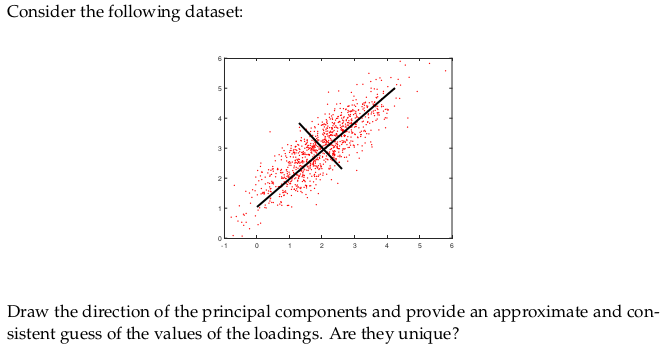
\includegraphics[width=1\textwidth]{images/Bias-Variance Tradeoff_01.png}}%
            %\caption{Nielsen's heuristics evaluation summary}
            %\label{BarsNielsenCrop}
        \end{minipage}
    \end{figure}
    \fbox{\begin{minipage}{\linewidth}
        Let's try to give some numbers to these PCs.\\
        $(0.5\,\,0.5)^T$, is this an eigenvector? No, an eigenvector has norm=1, here $\sqrt{0.5^2+0.5^2}=\sqrt{0.5}$\\
        As first PC is 45°/$\frac{\pi}{4}$:
        $$(\frac{\sqrt{2}}{2}\hspace{0.5em}-\frac{\sqrt{2}}{2})$$
        $$(\frac{\sqrt{2}}{2}\hspace{1.5em}\frac{\sqrt{2}}{2})$$
        They are orthogonal and have norm=1, properties for being PCs. They are not unique, just play with the signs, same direction, different verse
    \end{minipage}}

\subsubsection{PCA loadings}
    You are analysing a dataset where each observation is an age, height, length and width of a turtle. You want to know if the data can be well described by fewer than four dimensions, so you decide to do PCA. Which of the following is most likely to be the loadings of the first PC?
    \begin{enumerate}
        \item $(1,1,1,1)$
        \item $(0.5,0.5,0.5,0.5)$
        \item $(0.71,-0.71,0,0)$
        \item $(1,-1,-1,-1)$
    \end{enumerate}
    \fbox{\begin{minipage}{\linewidth}
        We check the norm: the options 1 and 4 have norms that exceed 1. The most likely correct one is the 2 as we expect this particular set of four variables to be positively correlated with each other in the first PC
    \end{minipage}}

\subsubsection{K-nearest neighbour for classification}
    A KNN classifier classifies a new data point by applying a mojirty voting among its K-nearest neighbour. There are the available data points in the dataset:

    \vspace{1em}
    $
    x_0=(-2,-3,0),\,y_0=1   \hspace{6em}    x_1=(-2,2,-1),\,y_1=1\\
    x_2 = (-2, -1, -3),\,y_2 = 1   \hspace{6em}    x_3 = (2, 1, -4),\,y_3 = 1\\
    x_4 = (2, -3, 2),\,y_4 = 1   \hspace{6em}    x_5 = (1, 2, 2),\,y_5 = 0\\
    x_6 = (-1, 1, -2),\,y_6 = 0   \hspace{6em}    x_7 = (-1, 2, 2),\,y_7 = 1\\
    x_8 = (1, -2, 0),\,y_8 = 0   \hspace{6em}    x_9 = (-3, -3, -2),\,y_9 = 1
    $

    \vspace{1em}
    Classify the new point $x=(0,0,-1)$ according to a KNN classifier trained on the dataset reported, assuming a $K=3$ and using the Euclidean distance

    \fbox{\begin{minipage}{\linewidth}
        We compare all Euclidean distances

        \vspace{1em}
        $
        d(x,x_0)=\sqrt{(0-(-2))^2+(0-(-3))^2+(-1-0)^2}=\sqrt{4+9+1}=\sqrt{14}=3.74\\
        d(x,x_1)=\sqrt{12}=3.46\\
        d(x,x_2)=\sqrt{9}=3\\
        d(x,x_3)=\sqrt{14}=3.74\\
        d(x,x_4)=\sqrt{22}=4.69\\
        d(x,x_5)=\sqrt{14}=3.74\\
        d(x,x_6)=\sqrt{3}=1.73\\
        d(x,x_7)=\sqrt{14}=3.74\\
        d(x,x_8)=\sqrt{6}=2.45\\
        d(x,x_9)=\sqrt{19}=4.36
        $

        \vspace{1em}
        The closest $K=3$ points are $(x_6,x_8,x_2)$, we perform a majority voting within $(y_6,y_8,y_2)=(0,0,1)$, which classifies the new point as 0
    \end{minipage}}

    What happens if $K=10$ instead? Is it a good idea?

    \fbox{\begin{minipage}{\linewidth}
        Since in this case |dataset|=10, if we have more 1's we will always predict 1, if more 0's always zero, so it is a bad idea, always selecting the same class for any point.\\
        Also for good practice we should select an odd value for $K$ in order to avoid ties when doing majority voting
    \end{minipage}}

\subsection{PAC-Learning and VC Dimension}
\subsubsection{VC dimension}
    Show that the VC dimension af an axis aligned rectangle is 4.

    \fbox{\begin{minipage}{\linewidth}
        Two steps:
        \begin{enumerate}
            \item Player 1 chooses $n$ points
            \item Player 2 opponent has to label the points, labelling done in order to let the first player to classify points
        \end{enumerate}
        If player 1 wins, VC dimension at least $n$, else we cannot say anything.\\
        In order to prove VC is a specific number, player 1 must win, otherwise we must show that all possible combinations of points in the space won't let player 1 win: \textbf{check true show one, check false show all}. We want to show
        $$
        VC(C)=4\Rightarrow
        \begin{cases}
            VC(C)\geq 4\\
            VC(C)< 5
        \end{cases}
        $$
        \begin{itemize}
            \item $\mathbf{VC(C)\geq 4}$, P1 chooses $n=4$ points (notice he should not choose align points, otherwise impossible for some combinations), then P2 labels them, for example\\
            \begin{center}
                
\includegraphics[width=0.3\textwidth]{images/Bias-Variance Tradeoff_02.png}           
            \end{center}
            In this way we can always separate with a rectangle, P1 always wins (he was smart by choosing non aligned points).\\
            It is possible to show by enumeration that all possible labelling are shattered by the rectangle
            \item $\mathbf{VC(C) < 5}$, consider 5 points and the set of points with maximum and minimum $x$ coordinate and maximum and minimum $y$ coordinates (the ones that make a perimeter): P2 can now label the one inside the perimeter with - and the ones on the perimeter with +, making the shattering impossible. This is true even if two aligned\\
            \begin{center}
                
\includegraphics[width=0.3\textwidth]{images/Bias-Variance Tradeoff_03.png}
                \hspace{1em}
                
\includegraphics[width=0.3\textwidth]{images/Bias-Variance Tradeoff_04.png}
            \end{center}
        \end{itemize}
    \end{minipage}}\

    Show that the VC dimension of a linear classifier in 2D is 3.

    \fbox{\begin{minipage}{\linewidth}
        $$
        VC(C)=3\Rightarrow
        \begin{cases}
            VC(C)\geq 3\\
            VC(C)< 4
        \end{cases}
        $$
        \begin{itemize}
            \item $\mathbf{VC(C)\geq 3}$, by considering a set of 3 non-aligned points, it is possible to show by enumeration that it is possible to shatter them with a linear classifier:
            \begin{center}
                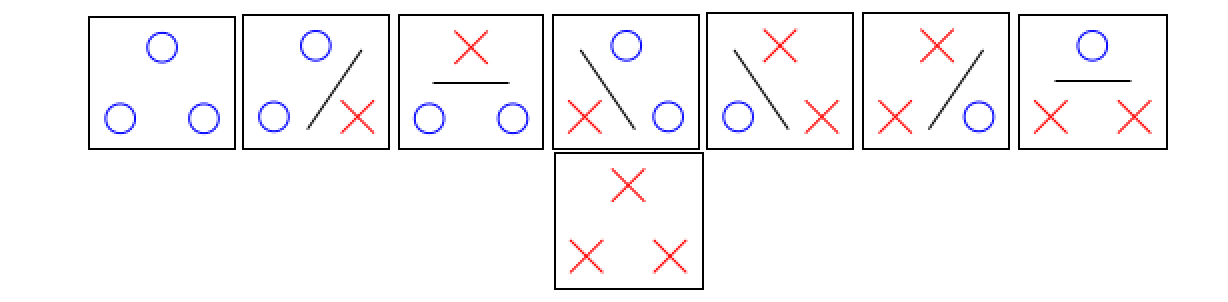
\includegraphics[width=0.9\textwidth]{images/Bias-Variance Tradeoff_05.png}           
            \end{center}
            \item $\mathbf{VC(C)< 4}$, we must show that it does not exists a set of 4 points which can be shattered by a linear classifier, consider the following cases:
            \begin{itemize}
                \item 4 aligned: alternating the instances from + to - we cannot shatter them
                \item 3 aligned: alternating the instances from + to - of the 3 aligned we cannot shatter them
                \item 4 on a convex hull: label the points on the two diagonals with opposite classes, we cannot shatter them
                \item 3 on a convex hull (triangle), 4-th inside it: the ones on the triangle same label, the inside one has the opposite label
            \end{itemize}
            \begin{center}
                
\includegraphics[width=0.9\textwidth]{images/Bias-Variance Tradeoff_06.png}           
            \end{center}
        \end{itemize}
    \end{minipage}}

    How many samples do you need to guarantee that the rectangle classifier provides you with an error larger than $\epsilon=0.1$ with probability smaller than $\delta=0.2$?

    \fbox{\begin{minipage}{\linewidth}
        Use the formula for VC:

        \vspace{1em}
        $
        N\geq\frac{1}{\epsilon}\left(
            4\log_2\left(\frac{2}{\delta}\right)+8VC(H)\log_2\left(\frac{13}{2}\right)
        \right)
        \\
        N\geq 10(4\log_2(10)+8*4\log_2(130))
        \\
        N\geq \left\lceil 10(4*4+32*7) \right\rceil
        \\
        N\geq 2400
        $

        \vspace{1em}
    \end{minipage}}

\subsubsection{PAC bound}
    Consider the hypothesis space of the decision trees with attributes with $n=4$ binary features with at most $k=10$ leaves (in this case you have less than $n^{k-1}2^{2k-1}$ different trees) and the problem of binary classification.\\
    Suppose you found a learning algorithm which is able to perfectly classify a training set of $N=1000$ samples. What is the lowest error $\epsilon$ you can guarantee to have with probability greater than $1-\delta=0.95$? How many samples do you need to halve this error?

    \fbox{\begin{minipage}{\linewidth}
        $$N\geq\frac{1}{\epsilon}\left(\ln|H|+\ln(\frac{1}{\delta})\right)$$
        We want to find $\epsilon$

        \vspace{1em}
        $
        \epsilon\geq\frac{1}{N}\left(\ln|H|+\ln(\frac{1}{\delta})\right)
        \\\cdots=\frac{1}{1000}\left(
            \ln (4^{10-1}2^{2*10-1})+\ln (\frac{1}{0.05})
        \right)
        \\\cdots=\frac{1}{1000}\left(
            \ln (4^92^{19})+\ln (\frac{1}{0.05})
        \right)
        \\\cdots=0.0286
        $

        \vspace{1em}
        To halve this error, we would need just need to double the number of samples we had originally, still requiring to have a perfect classifier on the new training set
    \end{minipage}}

    Another classifier is able only to get an error of $L_{train}(h)=0.02$ on your original training set. It is possible to use the same error bound derived in the first case? If not, derive a bound with the same probability for this case. How many samples do we need to halve the error bound?

    \fbox{\begin{minipage}{\linewidth}
        Agnostic learning since we cannot use the previous bound, the classifier is not able to perfectly classify all the points in the training set ($L_{train}\neq 0$)
        $$Pr(\exists\,\,h\,\in H|L_{true}(h)-L_{train}(h)>\epsilon)\leq|H|e^{-2N\epsilon^2}$$
        Thus the error bound is
        $$err=L_{true}=L_{train}+\epsilon\leq\underset{Bias}{\underbrace{L_{train}(h)}}+\underset{Variance}{\underbrace{\sqrt{\frac{\ln|H|+\ln\frac{1}{\delta}}{2N}}}}$$
        $
        \\\cdots=0.02+\sqrt{\frac{0.0286}{2}}
        \\\cdots=0.1397
        $

        \vspace{1em}
        To halve this error we solve for $N$
        $$L_{train}(h)+\sqrt{\frac{\ln|H|+\ln\frac{1}{\delta}}{2N}}\leq \frac{0.1397}{2}\Rightarrow N\geq 5766.34\sim 5767$$
    \end{minipage}}

\subsection{Kernel methods}
\subsubsection{SVM}
    Consider the linear two-class SVM classifier defined by the parameters $w=[2\,\,1],\,\,b=1$. Is the point $x_1=[-2\,\,4]$ a support vector?

    \fbox{\begin{minipage}{\linewidth}
        A point is a support vector if $|w^Tx+b|\leq 1$
        $$|w^Tx+b|=|-4+4+1|=1$$
        So it is a support vector
    \end{minipage}}

    Provide the analytical formula of the boundary and the margins.

    \fbox{\begin{minipage}{\linewidth}
        $$
        \begin{cases}
            2x_1+1x_2+1=0\text{\hspace{1em}(boundary)}\\
            2x_1+x_2+1=1\text{\hspace{1.5em}(positive margin)}\\
            2x_1+x_2+1=-1\text{\hspace{0.75em}(negative margin)}\\
        \end{cases}
        $$
    \end{minipage}}

    Give an example of a point which is on the boundary of the SVM

    \fbox{\begin{minipage}{\linewidth}
        A point on the boundary has to satisfy $w^Tx+b=0$, we can consider $x_{11}=0$ and solve
        $$2*0+1x_{22}+1=0\rightarrow x_{22}=-1$$
        So $x=[0\,\,-1]$ is on the boundary
    \end{minipage}}

    How the point $x_2=[3\,\,-1]$ is classified according to the trained SVM?

    \fbox{\begin{minipage}{\linewidth}
        $$w^Tx_2+b=2*3-1*1+1=6$$
        As binary classifier and positive, the point is classified in the positive class
    \end{minipage}}

    Assume to collect a new sample $x_3=[-1\,\,2]$ in the negative class, do we need to retrain the SVM?

    \fbox{\begin{minipage}{\linewidth}
        $$w^Tx_3+b=-2+2+1=1$$
        The point is missclassified, which means that $x_3$ would be a support vector thus we need to retrain the model
    \end{minipage}}

    Let us suppose we collect new data that make the classification task not linearly separable. How would you change the SVM model to deal with the task?

    \fbox{\begin{minipage}{\linewidth}
        We could either consider a soft-margin SVM or a different kernel function. In any case we should retrain the model to update the paramaters accordingly.
    \end{minipage}}

\subsection{Markov Decision Processes}
\subsubsection{Examples of MDPs}
    For each of the following dichotomies in MDP modeling provide examples of problems with the listed characteristics:
    \begin{tabularx}{\linewidth}{X|X|X|X}
        \toprule
        \endfirsthead
        \toprule
        \textbf{} & \textbf{} & \textbf{} & \textbf{}\\
        \midrule
        \endhead
        \footnotesize [Continues on next page]
        \endfoot
        \bottomrule
        \endlastfoot
        %body
        \textbf{Finite actions} & Robotic navigation (up, down, left, right) & \textbf{Infinite actions} & Pole balancing with continuous space applied force\\ \midrule
        \textbf{Deterministic transitions} & Chess (given the opponent strategy) & \textbf{Stochastic transitions} & Blackjack\\ \midrule
        \textbf{Deterministic rewards} & Robot navigation (0 everywhere, 1 in the exit point) & \textbf{Stochastic rewards} & Ad banner allocation (depending on clicks)\\ \midrule
        \textbf{Finite horizon} & Carcassone (finite number of tiles) & \textbf{Infinite horizon} & Stock exchange\\ \midrule
        \textbf{Indefinite horizon} & Chess & & \\ \midrule
        \textbf{Stationary environment} & Robotic navigation & \textbf{Non-stationary environment} & Every game with another learner playing
    \end{tabularx}

\subsubsection{Value function}
    Consider the MDP with $\alpha=0.3,\,\,\beta=0.5,\,\,\gamma=1,\,\,r_{search}=2,\,\,r_{wait}=0$ and the following policy:
    $$\pi(s|H)=1$$
    $$\pi(s|L)=0.5$$
    $$\pi(r|L)=0.5$$
    Compute the value function where the MDP stops after two steps
    \begin{center}
        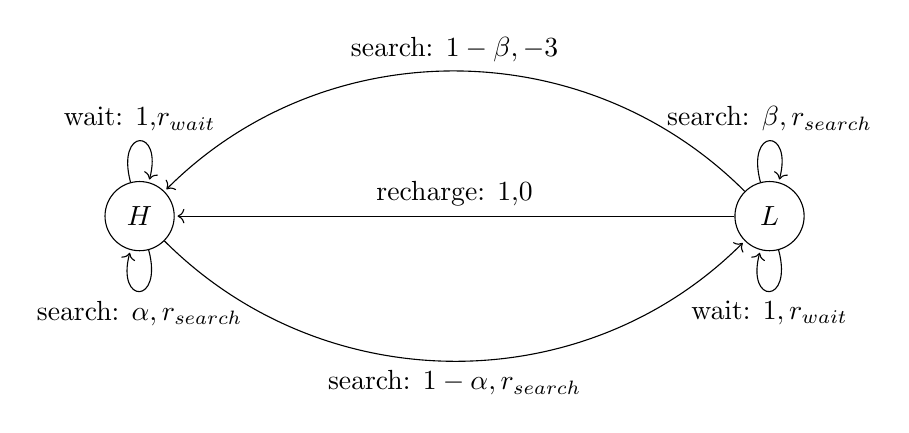
\begin{tikzpicture}[shorten >=1pt,node distance=8cm,on grid,auto]
            \node[state] (q_0) {$H$};
            \node[state] (q_1) [right=of q_0] {$L$};

            \path[->] 
            (q_0) %H%
                edge[loop above] node [swap] {wait: 1,$r_{wait}$} (q_0)
                edge[loop below] node [swap] {search: $\alpha,r_{search}$} (q_0)
                edge[out=315,in=225]  node [swap] {search: $1-\alpha,r_{search}$} (q_1)
            (q_1) %L%
                edge[loop above] node[swap] {search: $\beta,r_{search}$} (q_1)
                edge[loop below] node[swap] {wait: $1,r_{wait}$} (q_1)
                edge[out=180,in=0] node[swap] {recharge: 1,0} (q_0)
                edge[out=135,in=45] node[swap] {search: $1-\beta,-3$} (q_0)
            ;
        \end{tikzpicture}                
    \end{center}
    \fbox{\begin{minipage}{\linewidth}
        Use the Bellman expectation equation and operator
        $$V^\pi=\sum_{a \in A}\pi(a|s)\left(R(s,a)+\gamma\sum_{s'\in S}P(s'|s,a)V^\pi(s')\right)$$
        We first compute the immediate rewards, so stop at step 1 (so $P(s'|s,a)=0$ immediately)
        $$
        V^\pi=\sum_{a \in A}\pi(a|s)R(s,a)\Rightarrow
        \begin{cases}
            V^\pi(H)=\pi(s|H)R(H,s)=2\\
            V^\pi(L)=\pi(s|L)R(L,s)+\pi(r|L)R(L,r)
            \\\cdots=0.5*(\beta*2+(1-\beta)*(-3))+0.5*0
            \\\cdots=0.5*(0.5*2+0.5*(-3))
            \\\cdots=-0.25
        \end{cases}
        $$
        \begin{itemize}
            \item For $H$ as the policy only considers action $s$, only one member for the outer summation\\
            $
            V^\pi(H)=\pi(s|H)\left(
                R(H,s)+1(P(H|H,s)V^\pi(H)+P(L|H,s)V^\pi(L))
            \right)
            \\\cdots= 1\left(
                2+1(\alpha V^\pi(H)+(1-\alpha)V^\pi(L))
            \right)
            \\\cdots=2+0.3V^\pi(H)+0.7V^\pi(L)
            $\\
            Since we stop at step 2, we now consider the immediate reward and also $P(s'|s,a)=0$ as we stop
            $
            \\\cdots=2+0.3*2+0.7*(-0.25)=2.425
            $
            \item For $L$ we consider two terms in the outer summation\\
            $
            V^\pi(L)=\pi(s|L)\left(
                R(L,s)+1(P(L|L,s)V^\pi(L)+P(H|L,s)V^\pi(H))
            \right)
            \\+\pi(r|L)\left(
                R(L,r)+1(P(L|L,r)V^\pi(L)+P(H|L,r)V^\pi(H))
            \right)
            \\\cdots=0.5\left(
                \beta*2+(1-\beta)*(-3)+1(\beta V^\pi(L)+(1-\beta) V^\pi(H))
            \right)+0.5\left(
                0+1(0+1V^\pi(H))
            \right)
            \\\cdots=0.5\left(
                0.5*2+0.5*(-3)+0.5V^\pi(L)+0.5V^\pi(H)
            \right)+0.5V^\pi(H)
            \\\cdots=-0.25+0.25V^\pi(L)+0.25V^\pi(H)+0.5V^\pi(H)
            $\\
            Since we stop at step 2, we now consider the immediate reward and also $P(s'|s,a)=0$ as we stop
            $
            \\\cdots=-0.25+0.25*(-0.25)+0.75*2=1.1875
            $
        \end{itemize}
    \end{minipage}}

    What happens if we consider a discount factor of $\gamma=0.5$?

    \fbox{\begin{minipage}{\linewidth}
        Use the Bellman expectation equation and operator
        $$V^\pi=\sum_{a \in A}\pi(a|s)\left(R(s,a)+\gamma\sum_{s'\in S}P(s'|s,a)V^\pi(s')\right)$$
        The immediate rewards are unchanged
        $$
        V^\pi=\sum_{a \in A}\pi(a|s)R(s,a)\Rightarrow
        \begin{cases}
            V^\pi(H)=\pi(s|H)R(H,s)=2\\
            V^\pi(L)=\pi(s|L)R(L,s)+\pi(r|L)R(L,r)=-0.25
        \end{cases}
        $$
        \begin{itemize}
            \item For $H$ as the policy only considers action $s$, only one member for the outer summation\\
            $
            V^\pi(H)=\pi(s|H)\left(
                R(H,s)+0.5(P(H|H,s)V^\pi(H)+P(L|H,s)V^\pi(L))
            \right)
            \\\cdots= 1\left(
                2+0.5(\alpha V^\pi(H)+(1-\alpha)V^\pi(L))
            \right)
            \\\cdots=2+0.5(0.3V^\pi(H)+0.7V^\pi(L))
            $\\
            Since we stop at step 2, we now consider the immediate reward and also $P(s'|s,a)=0$ as we stop
            $
            \\\cdots=2+0.5(0.3*2+0.7*(-0.25))=2.2125
            $
            \item For $L$ we consider two terms in the outer summation\\
            $
            V^\pi(L)=\pi(s|L)\left(
                R(L,s)+0.5(P(L|L,s)V^\pi(L)+P(H|L,s)V^\pi(H))
            \right)
            \\+\pi(r|L)\left(
                R(L,r)+0.5(P(L|L,r)V^\pi(L)+P(H|L,r)V^\pi(H))
            \right)
            \\\cdots=0.5\left(
                \beta*2+(1-\beta)*(-3)+0.5(\beta V^\pi(L)+(1-\beta) V^\pi(H))
            \right)+0.5\left(
                0+0.5(0+1V^\pi(H))
            \right)
            \\\cdots=0.5\left(
                0.5*2+0.5*(-3)+0.5(0.5V^\pi(L)+0.5V^\pi(H))
            \right)+0.25V^\pi(H)
            \\\cdots=-0.25+0.125V^\pi(L)+0.125V^\pi(H)+0.25V^\pi(H)
            $\\
            Since we stop at step 2, we now consider the immediate reward and also $P(s'|s,a)=0$ as we stop
            $
            \\\cdots=-0.25+0.125*(-0.25)+0.375*2=0.46875
            $
        \end{itemize}
        Clearly the discounted value for the states is lower than the not discounted one, in the case we consider an MDP with finite time horizon.
    \end{minipage}}

    Compute the action-value function for each action value pair in the case the MDP stops after a single step

    \fbox{\begin{minipage}{\linewidth}
        Use the Bellman expectation equation and operator
        $$Q^\pi(s,a)=R(s,a)+\gamma\sum_{s' \in S}P(s'|s,a)\sum_{a' \in A}\pi(a'|s')Q^\pi(s',a')$$
        If it stops at the first step, we are computing the instantaneous reward
        $$
        Q^\pi(s,a)=R(s,a)\Rightarrow
        \begin{cases}
            Q(L,w)=1*0=0\\
            Q(L,s)=\beta*2+(1-\beta)*(-3)=-0.5\\
            Q(L,r)=1*0=0\\
            Q(H,w)=1*0=0\\
            Q(H,s)=\alpha*2+(1-\alpha)*2=2
        \end{cases}
        $$
    \end{minipage}}

\subsubsection{Bellman expectation equation for $V$}
    Provide the formulation of the Bellman expectation equation for $V$ equations for the MDP
    \begin{center}
        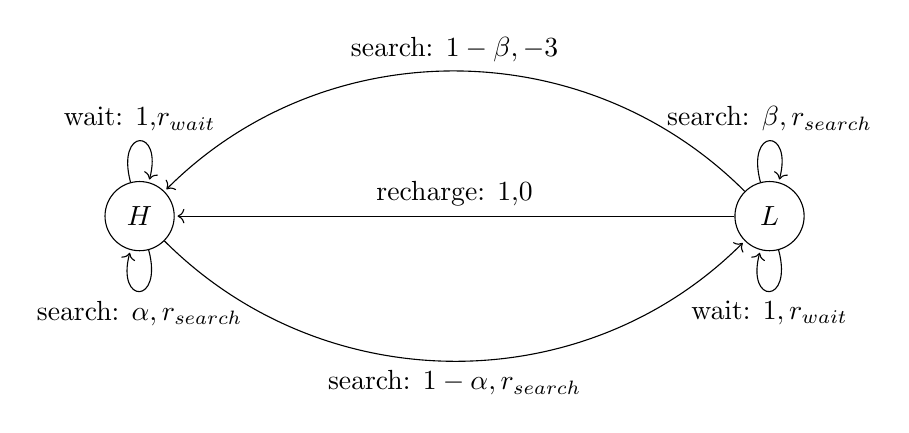
\begin{tikzpicture}[shorten >=1pt,node distance=8cm,on grid,auto]
            \node[state] (q_0) {$H$};
            \node[state] (q_1) [right=of q_0] {$L$};
    
            \path[->] 
            (q_0) %H%
                edge[loop above] node [swap] {wait: 1,$r_{wait}$} (q_0)
                edge[loop below] node [swap] {search: $\alpha,r_{search}$} (q_0)
                edge[out=315,in=225]  node [swap] {search: $1-\alpha,r_{search}$} (q_1)
            (q_1) %L%
                edge[loop above] node[swap] {search: $\beta,r_{search}$} (q_1)
                edge[loop below] node[swap] {wait: $1,r_{wait}$} (q_1)
                edge[out=180,in=0] node[swap] {recharge: 1,0} (q_0)
                edge[out=135,in=45] node[swap] {search: $1-\beta,-3$} (q_0)
            ;
        \end{tikzpicture}                
    \end{center}
    With $\alpha=0.2,\,\,\beta=0.1,\,\,r_{search}=2,\,\,r_{wait}=0,\,\,\gamma=0.9$ and in the case we consider the policy:
    $$\pi(H|s)=1$$
    $$\pi(L|r)=1$$
    \fbox{\begin{minipage}{\linewidth}
        Use the Bellman expectation equation and operator
        $$V^\pi=\sum_{a \in A}\pi(a|s)\left(R(s,a)+\gamma\sum_{s'\in S}P(s'|s,a)V^\pi(s')\right)$$
        $$V^\pi=R^\pi+\gamma P^\pi V^\pi$$
        We obtain

        $
        V^\pi(H)=\pi(H|s)\left(
            R(H,s)+0.9(P(H|H,s)V^\pi(H)+P(L|H,s)V^\pi(L))
        \right)
        \\\cdots=2+0.9(\alpha V^\pi(H)+(1-\alpha)V^\pi(L))
        \\\cdots=2+0.9(0.2V^\pi(H)+0.8V^\pi(L))\\
        V^\pi(L)=\pi(L|r)\left(
            R(L,r)+0.9(P(L|L,r)V^\pi(L)+P(H|L,r)V^\pi(H))
        \right)
        \\\cdots=0+0.9(0+1V^\pi(H))
        \\\cdots=0+0.9V^\pi(H)
        $

        Which in matrix form:
        $$
        V^\pi=
        \begin{bmatrix}
            2\\
            0
        \end{bmatrix}
        +0.9
        \begin{bmatrix}
            0.2 & 0.8\\
            1 & 0
        \end{bmatrix}
        V^\pi
        $$
    \end{minipage}}
    
\subsubsection{Transition matrix, value and action-value functions}
    \begin{center}
        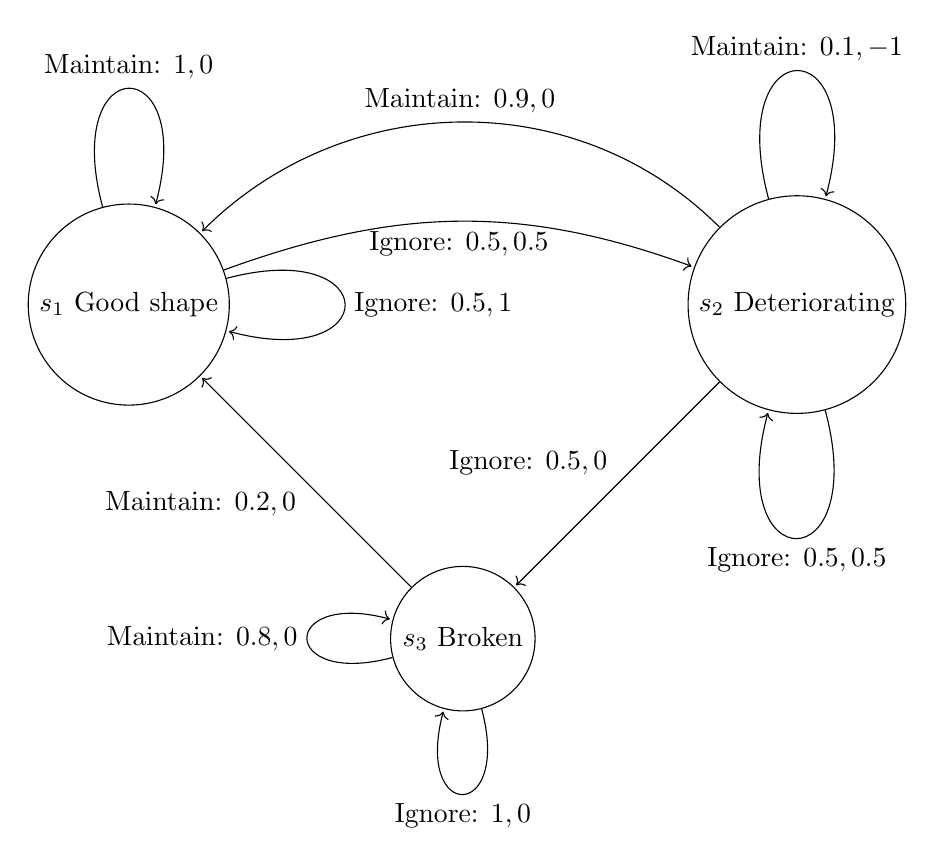
\begin{tikzpicture}[shorten >=1pt,node distance=6cm,on grid,auto]
            \node[state] (q_0) {$s_1$ Good shape};
            \node[state] (q_2) [below right=of q_0] {$s_3$ Broken};
            \node[state] (q_1) [above right=of q_2] {$s_2$ Deteriorating};

            \path[->] 
            (q_0) %s_1%
                edge[loop above] node[swap] {Maintain: $1,0$} (q_0)
                edge[loop right] node[swap] {Ignore: $0.5,1$} (q_0)
                edge[out=20,in=160] node[swap] {Ignore: $0.5,0.5$} (q_1)
            (q_1) %s_2%
                edge[loop above] node[swap] {Maintain: $0.1,-1$} (q_1)
                edge[out=135,in=45] node[swap] {Maintain: $0.9,0$} (q_0)
                edge[loop below] node[swap] {Ignore: $0.5,0.5$} (q_1)
                edge[out=225,in=45] node[swap] {Ignore: $0.5,0$} (q_2)
            (q_2) %s_3%
                edge[loop below] node[swap] {Ignore: $1,0$} (q_2)
                edge[loop left] node[swap] {Maintain: $0.8,0$} (q_2)
                edge[out=135,in=315] node[below left] {Maintain: $0.2,0$} (q_0)
            ;
        \end{tikzpicture}                
    \end{center}
    Provide the transition matrix for the policy $\pi(I|s_1)=1,\,\,\pi(M|s_2)=1,\,\,\pi(M|s_3)=1$

    \fbox{\begin{minipage}{\linewidth}
        We model a row as $[(S_i,a_1,S_0) (S_i,a_1,S_1) \cdots]$ and a column as $[(S_i,a_0,S_j) (S_i,a_1,S_j) \cdots]^T$.\\
        We follow this order for the actions: Ignore, Maintain
        $$
        P=
        \begin{bmatrix}
            0.5 & 0.5 & 0\\
            1 & 0 & 0\\
            0 & 0.5 & 0.5\\
            0.9 & 0.1 & 0\\
            0 & 0 & 1\\
            0.2 & 0 & 0.8
        \end{bmatrix}
        $$
        The policy tells us to keep the rows 1, 4 and 6:
        $$
        P=
        \begin{bmatrix}
            0.5 & 0.5 & 0\\
            0.9 & 0.1 & 0\\
            0.2 & 0 & 0.8
        \end{bmatrix}
        $$
    \end{minipage}}

    Provide the expected instantaneous reward for the previous policy

    \fbox{\begin{minipage}{\linewidth}
        We consider only those three transictions, the instantaneous rewards are
        $$
        R=
        \begin{bmatrix}
            0.5*1+0.5*0.5\\
            0.1*-1+0.9*0\\
            0.8*0+0.2*0
        \end{bmatrix}
        =
        \begin{bmatrix}
            0.75\\
            -0.1\\
            0
        \end{bmatrix}
        $$
    \end{minipage}}

    Compute the value function for the previous policy in the case the MDP stops after two steps with $\gamma=1$

    \fbox{\begin{minipage}{\linewidth}
        Use the Bellman expectation equation and operator
        $$V^\pi=\sum_{a \in A}\pi(a|s)\left(R(s,a)+\gamma\sum_{s'\in S}P(s'|s,a)V^\pi(s')\right)$$
        \begin{itemize}
            \item $
            V^\pi(s_1)=R(s_1,I)+0.5V^\pi(s_1)+0.5V^\pi(s_2)
            \\\cdots=0.75+0.5V^\pi(s_1)+0.5V^\pi(s_2)
            \\\cdots=0.75+0.5*0.75+0.5*(-0.1)=1.075
            $
            \item $
            V^\pi(s_2)=R(s_2|M)+0.1V^\pi(s_1)+0.9V^\pi(s_2)
            \\\cdots=-0.1+0.9*0.75+0.1*(-0.1)=0.565
            $
            \item $
            V^\pi(s_3)=R(s_3|M)+0.2V^\pi(s_1)+0.8V^\pi(s_2)
            \\\cdots=0+0.2*0.75+0=0.15
            $
        \end{itemize}
    \end{minipage}}

    Compute the action-value function for each state-action pair in the case the MDP stops after a single step

    \fbox{\begin{minipage}{\linewidth}
        Use the Bellman expectation equation and operator
        $$Q^\pi(s,a)=R(s,a)+\gamma\sum_{s' \in S}P(s'|s,a)\sum_{a' \in A}\pi(a'|s')Q^\pi(s',a')$$
        If it stops at the first step, we are computing the instantaneous reward
        $$
        Q^\pi(s,a)=R(s,a)\Rightarrow
        \begin{cases}
            Q(s_1,I)=0.5*1+0.5*0.5=0.75\\
            Q(s_1,M)=1*0=0\\
            Q(s_2,I)=0.5*0.5+0.5*0=0.25\\
            Q(s_2,M)=0.1*(-1)+0.9*0=-0.1\\
            Q(s_3,I)=1*0=0\\
            Q(s_3,M)=0.8*0+0.2*0=0
        \end{cases}
        $$
    \end{minipage}}

\subsubsection{MDP $\gamma$}
    Consider an MDP with 3 states and 3 actions. Applying the policy $\pi$ we have the following action-value function $Q(s,a)$ when we consider discount factors $\gamma$:
    \begin{tabularx}{\linewidth}{X|c c c|c c c|c c c}
        \toprule
        \endfirsthead
        \toprule
        \midrule
        \endhead
        \midrule
        \footnotesize [Continues on next page]
        \endfoot
        \bottomrule
        \endlastfoot
        & & $\gamma=0.9$ & & & $\gamma=0.95$ & & & $\gamma=0.99$ &\\ \midrule
        & d & so & cm & d & so & cm & d & so & cm\\ \midrule
        s1 & 35 & 25 & 0 & 95 & 90 & 0 & 780 & 785 & 0\\ \midrule
        s2 & 55 & 0 & 45 & 120 & 0 & 125 & 810 & 0 & 825\\ \midrule
        s3 & 165 & 0 & 0 & 240 & 0 & 0 & 940 & 0 & 0
    \end{tabularx}
    Provide the optimal policy $\pi^*$ for each discount factor $\gamma$.

    \fbox{\begin{minipage}{\linewidth}
        Assuming that the policy $\pi$ is explorative enough (visits all states and tries all available actions) the optimal policy is the one which maximize the value function in each state:
        $$\pi^*(0.9)=(d,d,d)$$
        $$\pi^*(0.95)=(d,cm,d)$$
        $$\pi^*(0.99)=(so,cm,d)$$
    \end{minipage}}

    What is the expected reward for $\pi^*$ if the initial state distribution is (0.4, 0.4, 0.2)?

    \fbox{\begin{minipage}{\linewidth}
        The expected reward $R(\gamma)$ is given by $p^TV^*(\gamma)$
        $$R(0.9)=(0.4,0.4,0.2)^T(35,55,165)=14+22+33=69$$
        $$R(0.95)=(0.4,0.4,0.2)^T(95,125,240)=136$$
        $$R(0.99)=(0.4,0.4,0.2)^T(785,825,940)=832$$
    \end{minipage}}

    Which $\gamma$ would you choose for this specific problem?

    \fbox{\begin{minipage}{\linewidth}
        This question does not make sense, the discount factor is not a parameter that should be chosen by the learner, but a characteristic of the MDP. The use of different values of $\gamma$ depends on the fact that the problem requires to be more far-sighted or myopic.
    \end{minipage}}

\subsection{Reinforcement Learning}
\subsubsection{MC and TD for state-value}
    Evaluate the value for the MDP with states $S=\{A,B,C\}$, $C$ is terminal with reward zero then, actions $A=\{h,r\}$ given the policy $\pi$ and the following trajectories:

    \vspace{1em}
    $(A,h,3)\rightarrow(B,r,2)\rightarrow(B,h,1)\rightarrow(C)$\\
    $(A,h,2)\rightarrow(A,h,1)\rightarrow(C)$\\
    $(B,r,1)\rightarrow(A,h,1)\rightarrow(C)$
    
    \vspace{1em}
    Can you tell without computing anything if by resorting to MC every-visit and first-visit approach you will have different results?

    \fbox{\begin{minipage}{\linewidth}
        Yes, in the first episode $B$ repeated twice, and in the third $A$ repeated twice, so different estimate
    \end{minipage}}

    Compute the values with the two aforementioned methods

    \fbox{\begin{minipage}{\linewidth}
        For MC:
        $$V(s_t)\leftarrow V(s_t)+\alpha (v_t-V(s_t))$$
        \begin{itemize}
            \item \textbf{First visit}
            $$
            V(A)=
            \begin{cases}
                \mathbf{(A,h,3)\rightarrow(B,r,2)\rightarrow(B,h,1)\rightarrow(C)\Rightarrow 6}\\
                \mathbf{(A,h,2)\rightarrow(A,h,1)\rightarrow(C)\Rightarrow 3}\\
                (B,r,1)\rightarrow\mathbf{(A,h,1)\rightarrow(C)\Rightarrow 1}\\
            \end{cases}
            = 10/3
            $$
            $$
            V(B)=
            \begin{cases}
                (A,h,3)\rightarrow\mathbf{(B,r,2)\rightarrow(B,h,1)\rightarrow(C)\Rightarrow 3}\\
                (A,h,2)\rightarrow(A,h,1)\rightarrow(C)\mathbf{\Rightarrow 0,\,\,not\,\,considered}\\
                \mathbf{(B,r,1)\rightarrow(A,h,1)\rightarrow(C)\Rightarrow 2}\\
            \end{cases}
            = 5/2
            $$
            \item \textbf{Every visit}
            $$
            V(A)=
            \begin{cases}
                \mathbf{(A,h,3)\rightarrow(B,r,2)\rightarrow(B,h,1)\rightarrow(C)\Rightarrow 6}\\
                \begin{cases}
                    \mathbf{(A,h,2)\rightarrow(A,h,1)\rightarrow(C)\Rightarrow 3}\\
                    (A,h,2)\rightarrow\mathbf{(A,h,1)\rightarrow(C)\Rightarrow 1}
                \end{cases}\\
                (B,r,1)\rightarrow\mathbf{(A,h,1)\rightarrow(C)\Rightarrow 1}
            \end{cases}
            = 11/4
            $$
            $$
            V(B)=
            \begin{cases}
                \begin{cases}
                    (A,h,3)\rightarrow\mathbf{(B,r,2)\rightarrow(B,h,1)\rightarrow(C)\Rightarrow 3}\\
                    (A,h,3)\rightarrow(B,r,2)\rightarrow\mathbf{(B,h,1)\rightarrow(C)\Rightarrow 1}
                \end{cases}\\
                (A,h,2)\rightarrow(A,h,1)\rightarrow(C)\mathbf{\Rightarrow 0,\,\,not\,\,considered}\\
                \mathbf{(B,r,1)\rightarrow(A,h,1)\rightarrow(C)\Rightarrow 2}
            \end{cases}
            = 6/3 = 2
            $$
        \end{itemize}
    \end{minipage}}

    Assume to consider a discount factor $\gamma=1$ and compute the values resorting to TD. Assume to start from zero values for each state and $\alpha=0.1$

    \fbox{\begin{minipage}{\linewidth}
        For TD:
        $$V(s_t)\leftarrow V(s_t)+\alpha (r_{t+1}+\gamma V(s_{t+1})-V(s_t))$$
        As we start from zero values, consider transition of episode 1
        $$(A,h,3)\rightarrow(B,r,2)\rightarrow(B,h,1)\rightarrow(C)$$
        
        $(A,h,3)\rightarrow(B,h,1)$
        $$V(A)=\underset{Initially\,\,all\,\,zero\,\,for\,\,A}{\underbrace{0}}+0.1(3+1*\underset{State\,B\,\,initially\,\,zero}{\underbrace{0}}-0)=0.3$$

        $(B,r,2)\rightarrow(B,h,1)$
        $$V(B)=0+0.1(2+1*0-0)=0.2$$

        $(B,h,1)\rightarrow(C)$
        $$V(B)=\underset{V(B)\,\,from\,\,step\,\,before}{\underbrace{0.2}}+0.1*(1+1*0-0.2)$$
        And so on...
    \end{minipage}}

\subsubsection{MC policy evaluation, improvement with $\epsilon$-greedy}
    Consider the set of trajectories below with discount factor $\gamma=1$

    \vspace{1em}
    $(A,u,2)\rightarrow(B,d,-2)\rightarrow(A,d,-2)\rightarrow(A,u,4)\rightarrow(C)$\\
    $(A,d,1)\rightarrow(B,u,-3)\rightarrow(C)$\\
    $(A,d,7)\rightarrow(B,d,0)\rightarrow(C)$

    \vspace{1em}
    Provide the policy evaluation step according to MC first-visit.

    \fbox{\begin{minipage}{\linewidth}
        $$
        Q(A,u)=
        \begin{cases}
            \mathbf{(A,u,2)\rightarrow(B,d,-2)\rightarrow(A,d,-2)\rightarrow(A,u,4)\rightarrow(C)\Rightarrow 2}\\
            (A,d,1)\rightarrow(B,u,-3)\rightarrow(C)\mathbf{\Rightarrow not\,\,considered}\\
            (A,d,7)\rightarrow(B,d,0)\rightarrow(C)\mathbf{\Rightarrow not\,\,considered}
        \end{cases}
        = 2
        $$
        And so on...
        $$
        \begin{cases}
            Q(A,u)=-2\\
            Q(B,u)=-3\\
            Q(A,d)=\frac{2-2+7}{3}=\frac{7}{3}\\
            Q(B,d)=\frac{0+0}{2}=0
        \end{cases}
        $$
    \end{minipage}}

    Provide the policy improvement step, i.e., the policy that the algorithm will deploy at the next iteration.

    \fbox{\begin{minipage}{\linewidth}
        In MC policy iteration we have to ensure sufficient exploration by deploying $\epsilon$-greedy policy, i.e.:
        $$
        \begin{cases}
            \pi(u|A)=\epsilon\\
            \pi(d|A)=1-\epsilon\\
            \pi(u|B)=\epsilon\\
            \pi(d|B)=1-\epsilon
        \end{cases}
        $$
    \end{minipage}}

    Do you think the results would have changed with MC every-visit evaluation?

    \fbox{\begin{minipage}{\linewidth}
        The only state-action pair that occurs more than once in single trajectory is $(A,u)$, so:
        $$
        Q(A,u)=\frac{2+4}{2}=3
        $$
        And since $Q(A,u)>Q(A,d)$ the $\epsilon$-greedy policy will change with $\pi(u|A)=1-\epsilon$ and $\pi(d|A)=\epsilon$
    \end{minipage}}

\subsubsection{SARSA}
    Conside the trajectory below, which is obtained while running the SARSA algorithm in an MDP with three states $S=\{A,B,C\}$, two actions $A=\{u,d\}$ and discount factor $\gamma=1$.
    $$(A,u,2)\rightarrow(B,d,-2)\rightarrow(A,d,-2)\rightarrow(A,u,-1)\rightarrow(B,u,-3)\rightarrow(C,d,4)\rightarrow(B)$$
    Provide a consistent guess over the policy $\pi$ that has been used to draw the latter trajectory. Do you think it is a reasonable policy?

    \fbox{\begin{minipage}{\linewidth}
        A guess:

        \vspace{1em}
        $
        \pi(u|A)=2/3\hspace{2em}\pi(d|A)=1/3\\
        \pi(u|B)=1/2\hspace{2em}\pi(d|B)=1/2\\
        \pi(u|C)=0\hspace{3em}\pi(d|C)=1
        $

        \vspace{1em}
        We do not have enough data to reliably estimate the policy $\pi$. On the one hand, it is unreasonable to have a deterministic policy in the state C, as we should guarantee sufficient exploration for the SARSA algorithm to converge to the optimal policy. On the other hand, the policy in the states A, B seems to be overly randomized to be an $\epsilon$-greedy policy.
    \end{minipage}}

    Provide the policy evaluation step according to SARSA by considering zero initial value $Q(s,a)=0$ for every state-action pair, and learning rate $\alpha=0.5$

    \fbox{\begin{minipage}{\linewidth}
        SARSA uses TD:
        $$Q(s,a)\leftarrow Q(s,a)+\alpha(r+\gamma Q(s',a')-Q(s,a))$$
        Starting from null values, follow the order of the episodes, we have:

        \vspace{1em}
        $
        Q^\pi(A,u)=0+0.5(2+1Q^\pi(B,d)-0)=0.5*2=1\\
        Q^\pi(B,d)=0+0.5(-2+Q^\pi(A,d)-0)=-1\\
        Q^\pi(A,d)=0+0.5(-2+Q^\pi(A,u)-0)=0.5(-2+1)=-0.5\\
        Q^\pi(A,u)=1+0.5(-1+Q^\pi(B,u)-1)=0\\
        Q^\pi(B,u)=0+0.5(-3+Q^\pi(C,d)-0)=-1.5\\
        Q^\pi(C,d)=0+0.5(4+0-0)=2
        $
    \end{minipage}}

    Provide the policy improvement step, i.e., the policy $\pi'$ that the algorithm will deploy at the next iteration.

    \fbox{\begin{minipage}{\linewidth}
        With the SARSA algorithm we have to ensure sufficient exploration, e.g. by deploying $\epsilon$-greedy policy ($1-\epsilon$ probability to choose greedy action), thus we have:

        \vspace{1em}
        $
        \pi(u|A)=1-\epsilon\hspace{2em}\pi(d|A)=\epsilon\\
        \pi(u|B)=\epsilon\hspace{3.5em}\pi(d|B)=1-\epsilon\\
        \pi(u|C)=\epsilon\hspace{3.5em}\pi(d|C)=1-\epsilon
        $
    \end{minipage}}

\subsubsection{Q-learning}
    Consider the following episode obtained by an agent interacting with an MDP having two states $S=\{A,B\}$ and two actions $A=\{l,r\}$
    $$(A,l,1)\rightarrow(A,l,1)\rightarrow(A,r,0)\rightarrow(B,r,10)\rightarrow(B,l,0)\rightarrow(A,r,0)\rightarrow(B,l,0)\rightarrow(A)$$
    Execute the Q-learning algorithm on the given episode considering initial state-action values $Q(S,a)=0$ for every stat-action pair, learning rate $\alpha=0.5$ and discount factor $\gamma=1$

    \fbox{\begin{minipage}{\linewidth}
        Q-learning:
        $$Q(s,a)\leftarrow Q(s,a)+\alpha(r+\gamma \max_{a'\in A}Q(s',a')-Q(s,a))$$
        
        a)\hspace{1em}$(A,l,1)\rightarrow(A,l,1)$
        $$Q(A,l)=0+0.5(1+1*0-0)=0.5$$

        b)\hspace{1em}$(A,l,1)\rightarrow(A,r,0)$
        $$Q(A,l)=0.5+0.5(1+1*0.5-0.5)=1$$

        c)\hspace{1em}$(A,r,0)\rightarrow(B,r,10)$
        $$Q(A,r)=0+0.5(0+1*\underset{Max\,\,value\,\,from\,\,state\,\,B\,\,is\,\,0}{\underbrace{0}}-0)=0$$

        d)\hspace{1em}$(B,r,10)\rightarrow(B,l,0)$
        $$Q(B,r)=0+0.5(10+1*0-0)=5$$

        e)\hspace{1em}$(B,l,0)\rightarrow(A,r,0)$
        $$Q(B,l)=\underset{Q(B,l)\,\,0\,\,still}{\underbrace{0}}+0.5(0+1*\underset{Max\,\,from\,\,A\,\,is\,\,Q(A,l)}{\underbrace{1}}-0)=0.5$$

        f)\hspace{1em}$(A,r,0)\rightarrow(B,l,0)$
        $$Q(A,r)=0+0.5(0+1*\underset{Q(B,r)}{\underbrace{5}}-0)=2.5$$

        g)\hspace{1em}$(B,l,0)\rightarrow(A)$
        $$Q(B,l)=0.5+0.5(0+1*2.5-0.5)=1.5$$
        Result:
        $$
        \begin{cases}
            Q(A,l)=1\\
            Q(A,r)=2.5\\
            Q(B,l)=1.5\\
            Q(B,r)=5
        \end{cases}
        $$
    \end{minipage}}

    Provide the best policy according to the output of Q-learning

    \fbox{\begin{minipage}{\linewidth}
        We select greedy policy $\pi(S)\in\arg\max_{a\in\{l,r\}}Q(S,a)$ w.r.t. the state-action values obtained with Q-learning, which gives $\pi(A)=r,\,\,\pi(B)=r$
    \end{minipage}}

    Do you think the agent fully exploited the policy learned in the episode above? Make a consistent guess with the available information

    \fbox{\begin{minipage}{\linewidth}
        Since at the steps a), b), \textbf{(the action chosen for A is not r)} and e) g) \textbf{(the action chosen for B is not r)} the agent is not choosing the action that is maximizing the current estimate of the Q values, we can infer that the episode does involve some exploration
    \end{minipage}}

\subsubsection{Model MDP}
    We are given an Heating, Ventilation, and Air Conditioning (HVAC) in which the states are cold (c), medium (m), warm (w) temperature. We can perform three actions: heat(h), refrigerate (r) and do nothing (d). Assume to have the following partial episodes for the HVAC functioning
    $$(c,d,0)\rightarrow(c,h,1)\rightarrow(m,h,1)\rightarrow(m,h,-1)\rightarrow(w,r,1)\rightarrow(m,.,.)\rightarrow\cdots$$
    $$(m,r,-2)\rightarrow(c,h,-2)\rightarrow(c,h,1)\rightarrow(m,h,1)\rightarrow(m,h,1)\rightarrow(w,.,.)\cdots$$
    where a tuple $(S,A,R)$ corresponds to state, action and reward.\\
    Model it as an MDP.

    \fbox{\begin{minipage}{\linewidth}
        \begin{center}
            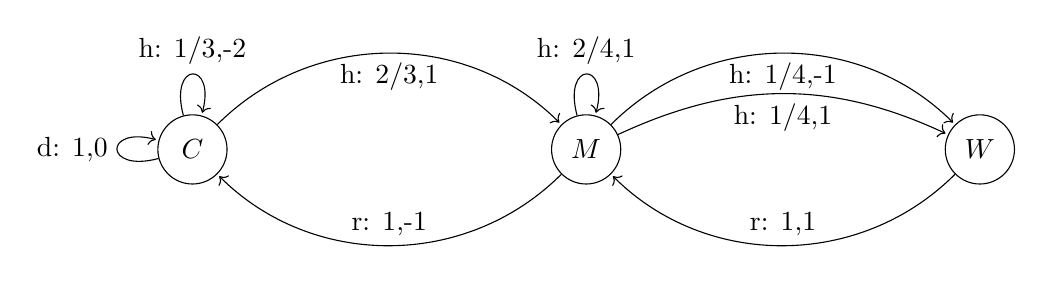
\begin{tikzpicture}[shorten >=1pt,node distance=5cm,on grid,auto]
                \node[state] (q_0) {$C$};
                \node[state] (q_1) [right=of q_0] {$M$};
                \node[state] (q_2) [right=of q_1]{$W$};
    
                \path[->] 
                (q_0) %C%
                    edge[loop left] node [swap] {d: 1,0} (q_0)
                    edge[out=45,in=135]  node [swap] {h: 2/3,1} (q_1)
                    edge[loop above] node[swap] {h: 1/3,-2} (q_0)
                (q_1) %M%
                    edge[loop above] node[swap] {h: 2/4,1} (q_1)
                    edge[out=45,in=135] node[swap] {h: 1/4,-1} (q_2)
                    edge[out=25,in=155] node[swap] {h: 1/4,1} (q_2)
                    edge[out=225,in=315] node[swap] {r: 1,-1} (q_0)
                (q_2) %W%
                    edge[out=225,in=315] node[swap] {r: 1,1} (q_1)
                ;
            \end{tikzpicture}                
        \end{center}
        Since two edges $M\rightarrow W$ through h, we merge the edges
        \begin{center}
            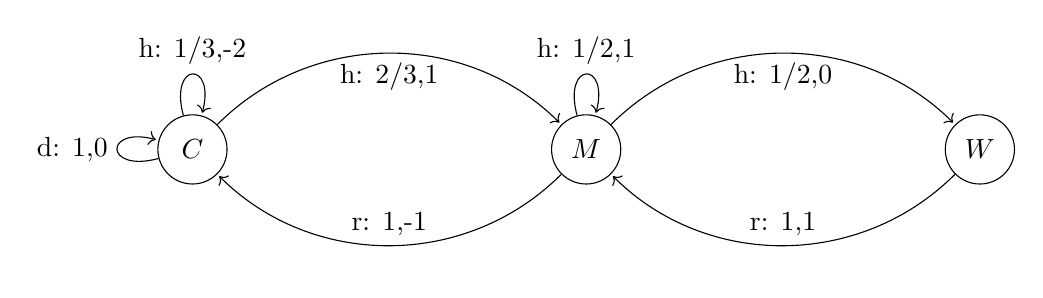
\begin{tikzpicture}[shorten >=1pt,node distance=5cm,on grid,auto]
                \node[state] (q_0) {$C$};
                \node[state] (q_1) [right=of q_0] {$M$};
                \node[state] (q_2) [right=of q_1]{$W$};
    
                \path[->] 
                (q_0) %C%
                    edge[loop left] node [swap] {d: 1,0} (q_0)
                    edge[out=45,in=135]  node [swap] {h: 2/3,1} (q_1)
                    edge[loop above] node[swap] {h: 1/3,-2} (q_0)
                (q_1) %M%
                    edge[loop above] node[swap] {h: 1/2,1} (q_1)
                    edge[out=45,in=135] node[swap] {h: 1/2,0} (q_2)
                    edge[out=225,in=315] node[swap] {r: 1,-1} (q_0)
                (q_2) %W%
                    edge[out=225,in=315] node[swap] {r: 1,1} (q_1)
                ;
            \end{tikzpicture}                
        \end{center}
    \end{minipage}}

    Can you tell if the reward of this process is stochastic or deterministic? And what about the transitions?

    \fbox{\begin{minipage}{\linewidth}
        The transitions are stochastic since some of the actions are leading to two different new states (e.g. action h in the state C). The reward is stochastic as well since heating in the M state provided once the reward 1 and once -1
    \end{minipage}}

    Assuming we want to evaluate the performance of the HVAC, tell which kind of problem we are in and suggest a technique to solve it

    \fbox{\begin{minipage}{\linewidth}
        This setting suggests it is an MDP prediction problem, either using directly the original episodes (sing MC or TD) or one might use the estimated model and use DP techniques to solve it in an exact way, due to the limited dimension of the problem
    \end{minipage}}

\subsection{ Multi-Armed Bandit}
\subsubsection{Minimum regret}
    Write the formula for the minimum regret we might have on average over $T=[e^{10}]$ time steps in the case we have a stochastic MAB with 3 arms and expected rewards:

    $R(a_1)=0.2$\\
    $R(a_2)=0.4$\\
    $R(a_3)=0.7$

    and each distribution $R(a_i)$ is a Bernoulli\\
    Not that the KL divergence for Bernoulli variables with means $p$ and $q$ is:
    $$KL(p,q)=p\log(\frac{p}{q})+(1-p)\log(\frac{(1-p)}{(1-q)})$$
    Is it possible that your algorithm achieves lower regret? If so, provide an example

    \fbox{\begin{minipage}{\linewidth}
        As we consider rewards, the optimal arm is $a_3$ with 0.7.\\
        Use the formula, if we assume that T is sufficiently large, we have:
        $$\lim_{T\rightarrow \infty}L_T=R_T\geq \log T\sum_{a_i\in A:\Delta_i>0}\frac{\Delta_i}{KL(R(a_i),R(a^*))}$$
        So:
        $$R_T\geq \log e^{10}\left(
            \frac{0.7-0.2}{KL(0.2,0.7)}
            +\frac{0.7-0.4}{KL(0.7-0.4)}
        \right)=\cdots=25.1528$$
        We might violate our lower bounds in some cases:
        \begin{itemize}
            \item If we consider a subset of MAB settings
            \item If we consider a single realization of rewards
        \end{itemize}
    \end{minipage}}

\subsubsection{Regret, pseudo-regret and UCB1}
    Consider a MAB algorithm choosing the arm $a_t$ and providing the following rewards $R_t$ over a time horizon $T=10$ rounds
    \begin{tabularx}{\linewidth}{c|X X X X X X X X X X}
        \toprule
        \endfirsthead
        \toprule
        \midrule
        \endhead
        \footnotesize [Continues on next page]
        \endfoot
        \bottomrule
        \endlastfoot
        %body
        $R_{1,t}$ & \textbf{0} & 1 & 1 & 0 & \textbf{0} & 1 & 0 & 1 & \textbf{0} & 0\\
        $R_{2,t}$ & 1 & \textbf{0} & 1 & 1 & 1 & 1 & \textbf{1} & 1 & 1 & \textbf{1}\\
        $R_{3,t}$ & 0 & 1 & \textbf{0} & \textbf{0} & 0 & \textbf{0} & 1 & \textbf{0} & 1 & 1\\ \midrule
        $a_t$ & 1 & 2 & 3 & 3 & 1 & 3 & 2 & 3 & 1 & 2
    \end{tabularx}
    (only the reward for the chosen arm is revealed to the algorithm). Moreover, assume that the expected value for the three arms' reward are $\mu_1=0.3,\,\,\mu_2=0.8,\,\,\mu_3=0.6$\\
    Compute the cumulated reward, the regret and the pseudo-regret for the algorithm over the time horizon $T$. (Recall that the regret is computed over realizations, while the pseudo-regret is computed over expected values)
    
    \fbox{\begin{minipage}{\linewidth}
        \begin{itemize}
            \item Look at the table, the highlighted numbers are the rewards that we got, so cumulated rewards is just sum of those values:
            $$0+0+0+0+0+0+1+0+0+1=2$$
            \item The regret is given by the optimal reward minus the one we got:
            $$10-2=8$$
            \item We use:
            $$L_T=\sum_{a_i\in A:\Delta_i>0}\mathbb{E}[N_T(a_i)]\Delta_i$$
            At each timestamp, the $\Delta$ are the same since we consider the expected values and not the realizations. As $\mu_2$ is the maximum among the three:
            $$
            \begin{cases}
                \Delta_1=\mu_2-\mu_1=0.8-0.3=0.5\\
                \Delta_1=\mu_2-\mu_1=0.8-0.3=0\\
                \Delta_3=\mu_2-\mu_3=0.8-0.6=0.2
            \end{cases}
            $$
            So the pseudo-regret is:
            $$0.5+0+0.2+0.2+0.5+0.2+0+0.2+0.5+0=2.3$$
        \end{itemize}
    \end{minipage}}

    Compute the values for the UCB1 bounds at time 5 for the three arms. Do you think that the algorithm used in this setting can be the UCB1?

    \fbox{\begin{minipage}{\linewidth}
        $$U(a_i):=\hat{R_t}(a_i)+B_t(a_i)\geq R(a_i)$$
        For UCB1:
        $$\hat{R}_t(al)=\frac{1}{N_t(a_l)}\sum_{j=1}^{t-1}r_{a_{i_j},j}1\{a_l=a_{i_j}\},\,\forall a_i\in A$$
        $$B_t(a_l)=\sqrt{\frac{2\log t}{N_t(a_l)}},\,\forall a_l\in A$$
        So:
        $$
        \begin{cases}
            U_{1,5}=\frac{0+0}{2}+\sqrt{\frac{2\log5}{2}}\\
            U_{2,5}=\frac{0}{1}+\sqrt{\frac{2\log5}{1}}\\
            U_{3,5}=\frac{0+0}{2}+\sqrt{\frac{2\log5}{2}}
        \end{cases}
        $$
        UCB1 tries to pull the arms the same number of times (plays the one that has maximum $U$ so usually lowest $N$), therefore the arm chosen for the next round would be 2. As in timestamp 6 the arm chosen is 3, the algorithm cannot be UCB1
    \end{minipage}}

    Do you think that the algorithm used in this setting might be Thompson sampling?

    \fbox{\begin{minipage}{\linewidth}
        Since the TS has a stochastic nature, there is the chance that any possible sequence of the arms is chosen, even if with a small probability. Therefore, the algorithm run above might be TS
    \end{minipage}}

\subsubsection{Thompson sampling and UCB1}
    Consider the Thompson Sampling algorithm. Assume to have the following posterior distributions $Beta(\alpha_t,\beta_t)$ for arms $A=\{a_1,\cdots,a_5\}$ rewards, which are distributed as Bernoulli:
    \begin{enumerate}[start=1,label={- $a$\arabic{*}:}]
        \item $\alpha_t=1\hspace{1em}\beta_t=5\hspace{1em}\hat{r}(a_1)=0.63$
        \item $\alpha_t=6\hspace{1em}\beta_t=4\hspace{1em}\hat{r}(a_2)=0.35$
        \item $\alpha_t=11\hspace{1em}\beta_t=23\hspace{1em}\hat{r}(a_3)=0.16$
        \item $\alpha_t=12\hspace{1em}\beta_t=33\hspace{1em}\hat{r}(a_4)=0.22$
        \item $\alpha_t=28\hspace{1em}\beta_t=21\hspace{1em}\hat{r}(a_5)=0.7$
    \end{enumerate}

    Which arm would the TS algorithm play for the next round?

    \fbox{\begin{minipage}{\linewidth}
        $a_5$ as it has the highest sampled value ($\hat{r}$)
    \end{minipage}}

    Do you think that there is an arm that is more promising to be the best one?

    \fbox{\begin{minipage}{\linewidth}
        In TS in case of success the $\alpha_t$ is increased, so we look at arms that have $\alpha_t>\beta_t$: either $a2$ or $a5$, probably $a5$ most promising as $\alpha_t-\beta_t=7$. If there was an arm with $\beta_t=1$ it meant that it never failed: it only provided positive samples, so best one
    \end{minipage}}

    Assume we started the TS algorithm with uniform $Beta(1,1)$ priors, what would UCB1 have chosen in the case of Bernoulli rewards for the next round?
    
    \fbox{\begin{minipage}{\linewidth}
        $$U(a_i):=\hat{R_t}(a_i)+B_t(a_i)\geq R(a_i)$$
        For UCB1:
        $$\hat{R}_t(al)=\frac{1}{N_t(a_l)}\sum_{j=1}^{t-1}r_{a_{i_j},j}1\{a_l=a_{i_j}\},\,\forall a_i\in A$$
        $$B_t(a_l)=\sqrt{\frac{2\log t}{N_t(a_l)}},\,\forall a_l\in A$$
        Since we started with uniform prior and at each round we collected a success or a failure we are currently at round:
        $$t=4+8+32+43+47=134$$
        while the UCB1 upper bound $U_t(a_i)$ is of the form:
        $$U_t(a_i)=\frac{\alpha_t-1}{\alpha_t+\beta_t-2}+\sqrt{\frac{2\log t}{\alpha_t+\beta_t-2}}$$
        $$U(a_1)=\frac{0}{4}+\sqrt{
            \frac{
                2\log 134
            }{
                4
            }
        }$$
        $$\vdots$$
        \vspace{0.5em}
    \end{minipage}}

\subsubsection{UCB confidence intervals}
    Consider the following bounds (supposed to hold with probability at least $\delta$) for a MAB stochastic setting
    \begin{center}
        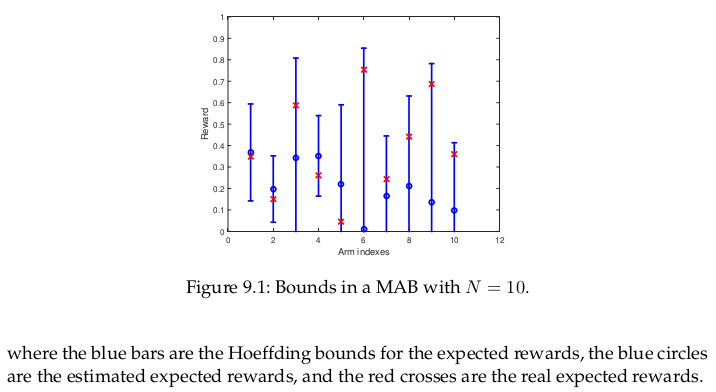
\includegraphics[width=1\textwidth]{images/mab_01.png}
    \end{center}
    \fbox{\begin{minipage}{\linewidth}
        \begin{enumerate}
            \item Which arm would a UCB1 algorithm choose for the next round? Arm 6, which has reward of zero and high bound
            \item Do you think that the figure might be the results obtained by running UCB1 for several rounds? No, UCB1 at each time is trying to keep all upper confidence bound at the same level, but here some arms pulled more times even though others should have been pulled before
            \item Which arm will UCB1 converge to if $T\rightarrow\infty$? Arm 6, since it is the one with highest expected value
            \item Which arm is the one which we pulled the most so far? Arms 2 and 4 as they have the smallest confidence bounds (which are inversely proportional to the number of pulls)
        \end{enumerate}
    \end{minipage}}
    
\end{document}